\documentclass[11pt,a4paper]{article}

% -----------------------------------------------------------------------------
% Packages
% -----------------------------------------------------------------------------
\usepackage[margin=2.5cm]{geometry}
\usepackage[T1]{fontenc}
\usepackage[utf8]{inputenc}
\usepackage{lmodern}
\usepackage{microtype}
\usepackage{graphicx}
\usepackage{booktabs}
\usepackage{array}
\usepackage{amsmath}
\usepackage{amssymb}
\usepackage{siunitx}
\usepackage{xcolor}
\usepackage{enumitem}
\usepackage{listings}
\usepackage{caption}
\usepackage{subcaption}
\usepackage{fancyhdr}
\usepackage[hidelinks]{hyperref}

% -----------------------------------------------------------------------------
% Document metadata and formatting
% -----------------------------------------------------------------------------
\newcommand{\reporttitle}{Patient-Specific Computational Fluid Dynamics of the Airways}
\newcommand{\reportsubtitle}{Segmentation, Mesh Generation, and Flow Analysis in Tracheomalacia}
\newcommand{\reportauthor}{Henri Van Overmeire}
\newcommand{\reportdate}{\today}

\definecolor{codebackground}{RGB}{245,247,250}
\definecolor{codekeyword}{RGB}{30,80,150}
\definecolor{codecomment}{RGB}{65,120,75}

\lstset{
  basicstyle=\ttfamily\small,
  backgroundcolor=\color{codebackground},
  keywordstyle=\color{codekeyword}\bfseries,
  commentstyle=\color{codecomment},
  frame=single,
  breaklines=true,
  columns=fullflexible,
  keepspaces=true,
  showstringspaces=false
}

\pagestyle{fancy}
\fancyhf{}
\fancyhead[L]{Airway CFD}
\fancyhead[R]{Henri Van Overmeire}
\fancyfoot[C]{\thepage}
\setlength{\headheight}{14pt}

\sisetup{
  detect-all,
  per-mode=symbol
}

\graphicspath{{figures/}}

\begin{document}
\hypersetup{pageanchor=false}

% -----------------------------------------------------------------------------
% Title page
% -----------------------------------------------------------------------------
\begin{titlepage}
  \centering
  \vspace*{2.5cm}

  {\Large Computational Biofluid Mechanics\par}
  \vspace{1.5cm}

  {\Huge\bfseries \reporttitle\par}
  \vspace{0.6cm}
  {\Large \reportsubtitle\par}

  \vfill

  \begin{tabular}{rl}
    \textbf{Author:} & \reportauthor \\
    \textbf{Date:}   & \reportdate \\
    \textbf{Repository:} &
    \href{https://github.com/henrivanovermeire/tracheomalacia_cfd/settings}
    {\texttt{github.com/henrivanovermeire/tracheomalacia\_cfd}}
  \end{tabular}

  \vfill

  \textit{Reproducible project report; analyses still in progress are identified
  explicitly in the text.}
\end{titlepage}

\hypersetup{pageanchor=true}
\pagenumbering{roman}

% -----------------------------------------------------------------------------
% Front matter
% -----------------------------------------------------------------------------
\begin{abstract}
Tracheomalacia is characterised by excessive collapse or narrowing of the
tracheal lumen and can substantially alter respiratory airflow. This project
uses patient-specific computed tomography, three-dimensional airway
segmentation, and computational fluid dynamics (CFD) to compare airflow before
and after intervention. Airway surfaces are segmented in 3D Slicer, clipped
along VMTK-derived centerlines, extended in the local centerline direction, and
closed with planar caps. Tetrahedral volume meshes are generated with Gmsh and
steady incompressible airflow is solved using OpenFOAM. This report documents
the reproducible processing pipeline, evaluates mesh quality and mesh
independence, and compares clinically relevant flow quantities between the
preoperative and postoperative geometries. The preoperative minimum lumen area
was \SI{1.813}{\milli\metre\squared}, compared with
\SI{5.169}{\milli\metre\squared} at the matched postoperative location, giving
an area constriction of 64.9\%. In the steady postoperative model the local
pressure drop was \SI{30.95}{\pascal}, the resistance was
\SI{15.41}{\pascal\per\litre\per\minute}, and 73.2\% of outlet flow entered the
right lung. A four-level HXT mesh study selected the \num{0.15}~mm mesh because
its reported metrics differed by no more than 2.02\% from the denser mesh while
using 48\% fewer cells. A complete-cycle transient calculation is configured;
its final phase-resolved results are reported only after solver completion.
\end{abstract}

\tableofcontents
\listoffigures
\listoftables
\clearpage
\pagenumbering{arabic}

% -----------------------------------------------------------------------------
\section{Introduction}
\label{sec:introduction}

Tracheomalacia involves reduced structural stability of the tracheal wall,
which may cause dynamic narrowing and increased respiratory resistance. While
medical imaging describes airway anatomy, CFD can quantify how geometric
narrowing influences velocity, pressure loss, flow distribution, and local
shear-related quantities.

The objectives of this project are to:

\begin{enumerate}[label=\arabic*.]
  \item construct patient-specific preoperative and postoperative airway
        geometries from computed tomography;
  \item establish a reproducible segmentation-to-simulation workflow;
  \item quantify airflow and pressure differences between the two cases; and
  \item assess whether the numerical conclusions are independent of mesh
        resolution.
\end{enumerate}

\subsection{Research questions}

\begin{itemize}
  \item How does the intervention change the minimum airway cross-section?
  \item How does the pressure drop across the trachea change?
  \item Where do peak velocities and recirculation regions occur?
  \item How is flow divided among the distal outlets?
  \item Are the reported quantities sufficiently mesh independent?
\end{itemize}

% -----------------------------------------------------------------------------
\section{Critical review of a selected CFD paper}
\label{sec:paper_review}

The selected paper is Taherian et al.'s patient-specific CFD evaluation of
excessive dynamic airway collapse before and after tracheal stenting
\cite{taherian2017}. Each of the five required subsections below is shorter than
150 words. No paper figures are reproduced, remaining within the permitted
maximum of three.

\subsection{Goal}

The study investigated whether patient-specific computational fluid dynamics
could quantify the functional consequences of excessive dynamic airway collapse
and assess improvement after tracheal stenting. The authors specifically
compared inspiratory and expiratory airflow before and after intervention using
CT-derived airway geometries. They aimed to determine how stenting affected
pressure loss, velocity, wall shear stress, and turbulence, and whether these
CFD quantities revealed clinically relevant changes that conventional pulmonary
function tests might miss. The underlying question was therefore not merely
whether the airway lumen became larger, but whether the anatomical intervention
produced a meaningful improvement in respiratory flow behaviour.

\subsection{Methods}

Four patient-specific airway models represented inspiration and expiration
before and after stenting. CT images were segmented in Mimics and simulated in
STAR-CCM+. Each rigid model included the trachea and approximately six to eight
airway generations. The authors simulated 2.5~s inspiration and 2.5~s expiration
with sinusoidal resting-breathing flow. Patient-specific outlet pressure
functions were derived in a preliminary step from lobar volume changes, while
the inlet was atmospheric with 10\% turbulence intensity. Unsteady RANS with a
low-Reynolds-number $k$--$\omega$ model and second-order spatial and temporal
schemes was used. Inlet and outlet extensions measured one and four hydraulic
diameters, respectively. Polyhedral meshes with prism layers were tested at
0.9, 1.7, and 3.2 million cells; 1.7 million cells was selected from pressure,
velocity, and wall-shear-stress sensitivity.

\subsection{Results}

Stenting produced the clearest improvement during expiration. The severe
pre-stent narrowing generated a high-velocity jet, recirculation, substantial
pressure loss, and elevated wall shear stress. The reported pre-/post-stent
expiratory pressure difference was approximately $26~\mathrm{cmH_2O}$, while
mean tracheal wall shear stress decreased from 3.98 to 0.793~Pa, an approximately
80\% reduction. Velocity variations also became smaller after stenting.
Inspiratory changes were comparatively minor; mean wall shear stress increased
from 0.0354 to 0.0813~Pa, and the stent introduced some local flow disturbance.
Turbulence intensity increased in parts of both phases after intervention.
Spirometry changed only modestly---FEV$_1$ increased by 290~mL---whereas CFD
exposed pronounced expiratory functional improvement that pulmonary function
testing did not clearly reflect.

\subsection{Limitations}

The study considered only one patient, so its quantitative findings cannot be
generalised to all patients with excessive dynamic airway collapse. The airway
walls were rigid even though wall deformation is the defining feature of the
disease. Separate end-inspiration and end-expiration geometries represented the
extremes of breathing rather than continuously moving anatomy; fluid--structure
interaction was omitted because patient-specific tissue properties were
unavailable. The upper airway and deeper peripheral generations were truncated,
although both may influence tracheal flow and outlet impedance. Outlet pressures
were inferred indirectly from lobar volume changes, and local CFD predictions
were not validated against invasive pressure or velocity measurements. The RANS
turbulence model and selected boundary conditions add model-form uncertainty.
Finally, mesh sensitivity was demonstrated primarily for selected quantities in
one pre-stent expiratory geometry.

\subsection{Evaluation}

For this patient, the authors largely answered their research question. The
paired pre-/post-stent and inspiration/expiration design isolated the phase in
which airway collapse mattered most, and pressure, velocity, and wall shear
stress changed coherently after intervention. The contrast with relatively
insensitive spirometry supports the claim that CFD can provide additional
functional information. The mesh test and patient-informed outlet conditions
strengthen the internal comparison. However, the study establishes a
patient-specific proof of concept rather than a validated diagnostic or
prognostic method. Rigid endpoint geometries cannot reproduce dynamic coupling
between airflow and collapse, and a single case cannot establish clinical
accuracy or treatment thresholds. Thus, the conclusion that stenting improved
this patient's expiratory airflow is supported, whereas broader claims about
CFD-guided management require validation in more patients with dynamic or
fluid--structure-interaction models.

% -----------------------------------------------------------------------------
\section{Imaging data and anatomical cases}
\label{sec:data}

Two computed-tomography datasets are analysed: a preoperative case and a
postoperative case. Table~\ref{tab:imaging} should be completed from the DICOM
metadata and segmentation logs.

\begin{table}[htbp]
  \centering
  \caption{Imaging and anatomical case information.}
  \label{tab:imaging}
  \begin{tabular}{@{}llll@{}}
    \toprule
    Case & Voxel dimensions & Voxel spacing (mm) & Clinical state \\
    \midrule
    Preoperative  & [insert] & [insert] & Before intervention \\
    Postoperative & [insert] & [insert] & After intervention \\
    \bottomrule
  \end{tabular}
\end{table}

All patient-derived data must be handled according to the applicable privacy,
ethics, and data-management requirements. No directly identifying information
should appear in this report or repository.

% -----------------------------------------------------------------------------
\section{Airway segmentation and surface preparation}
\label{sec:segmentation}

\subsection{Segmentation}

The CT series is loaded into 3D Slicer. A case-specific seed is placed in the
airway lumen, and connected region growth is performed within a selected
Hounsfield-unit interval. Thresholds and seed coordinates are stored under
\texttt{segmentation/assets/<case>/}. The result is inspected in axial,
coronal, sagittal, and three-dimensional views to exclude lung parenchyma and
external air while retaining the clinically relevant branches.

Record the final settings in Table~\ref{tab:segmentation}.

\begin{table}[htbp]
  \centering
  \caption{Final segmentation settings.}
  \label{tab:segmentation}
  \begin{tabular}{@{}llll@{}}
    \toprule
    Case & Lower HU & Upper HU & Segmented voxels \\
    \midrule
    Preoperative  & [insert] & [insert] & [insert] \\
    Postoperative & [insert] & [insert] & [insert] \\
    \bottomrule
  \end{tabular}
\end{table}

\subsection{Centerline extraction and clipping}

A centerline network is calculated using VMTK. Visually refined clipping points
are loaded as the Slicer markup node \texttt{AirwayCutEndpoints}. The airway is
clipped using the same \textit{Clip Vessel} logic as the SlicerVMTK user
interface, with \texttt{AirwayNetworkModel} providing the centerline direction.

Flow extensions are aligned with the local centerline and adapt to the airway
radius at each clipping location. Planar caps close the extensions for CFD. The
final Slicer model is \texttt{AirwayExtendedSurfaceCapped} and is exported as
\texttt{meshes/<case>/airways.stl}, preventing the two anatomies from
silently overwriting one another.

\begin{figure}[htbp]
  \centering
  \begin{subfigure}[t]{0.48\textwidth}
    \centering
    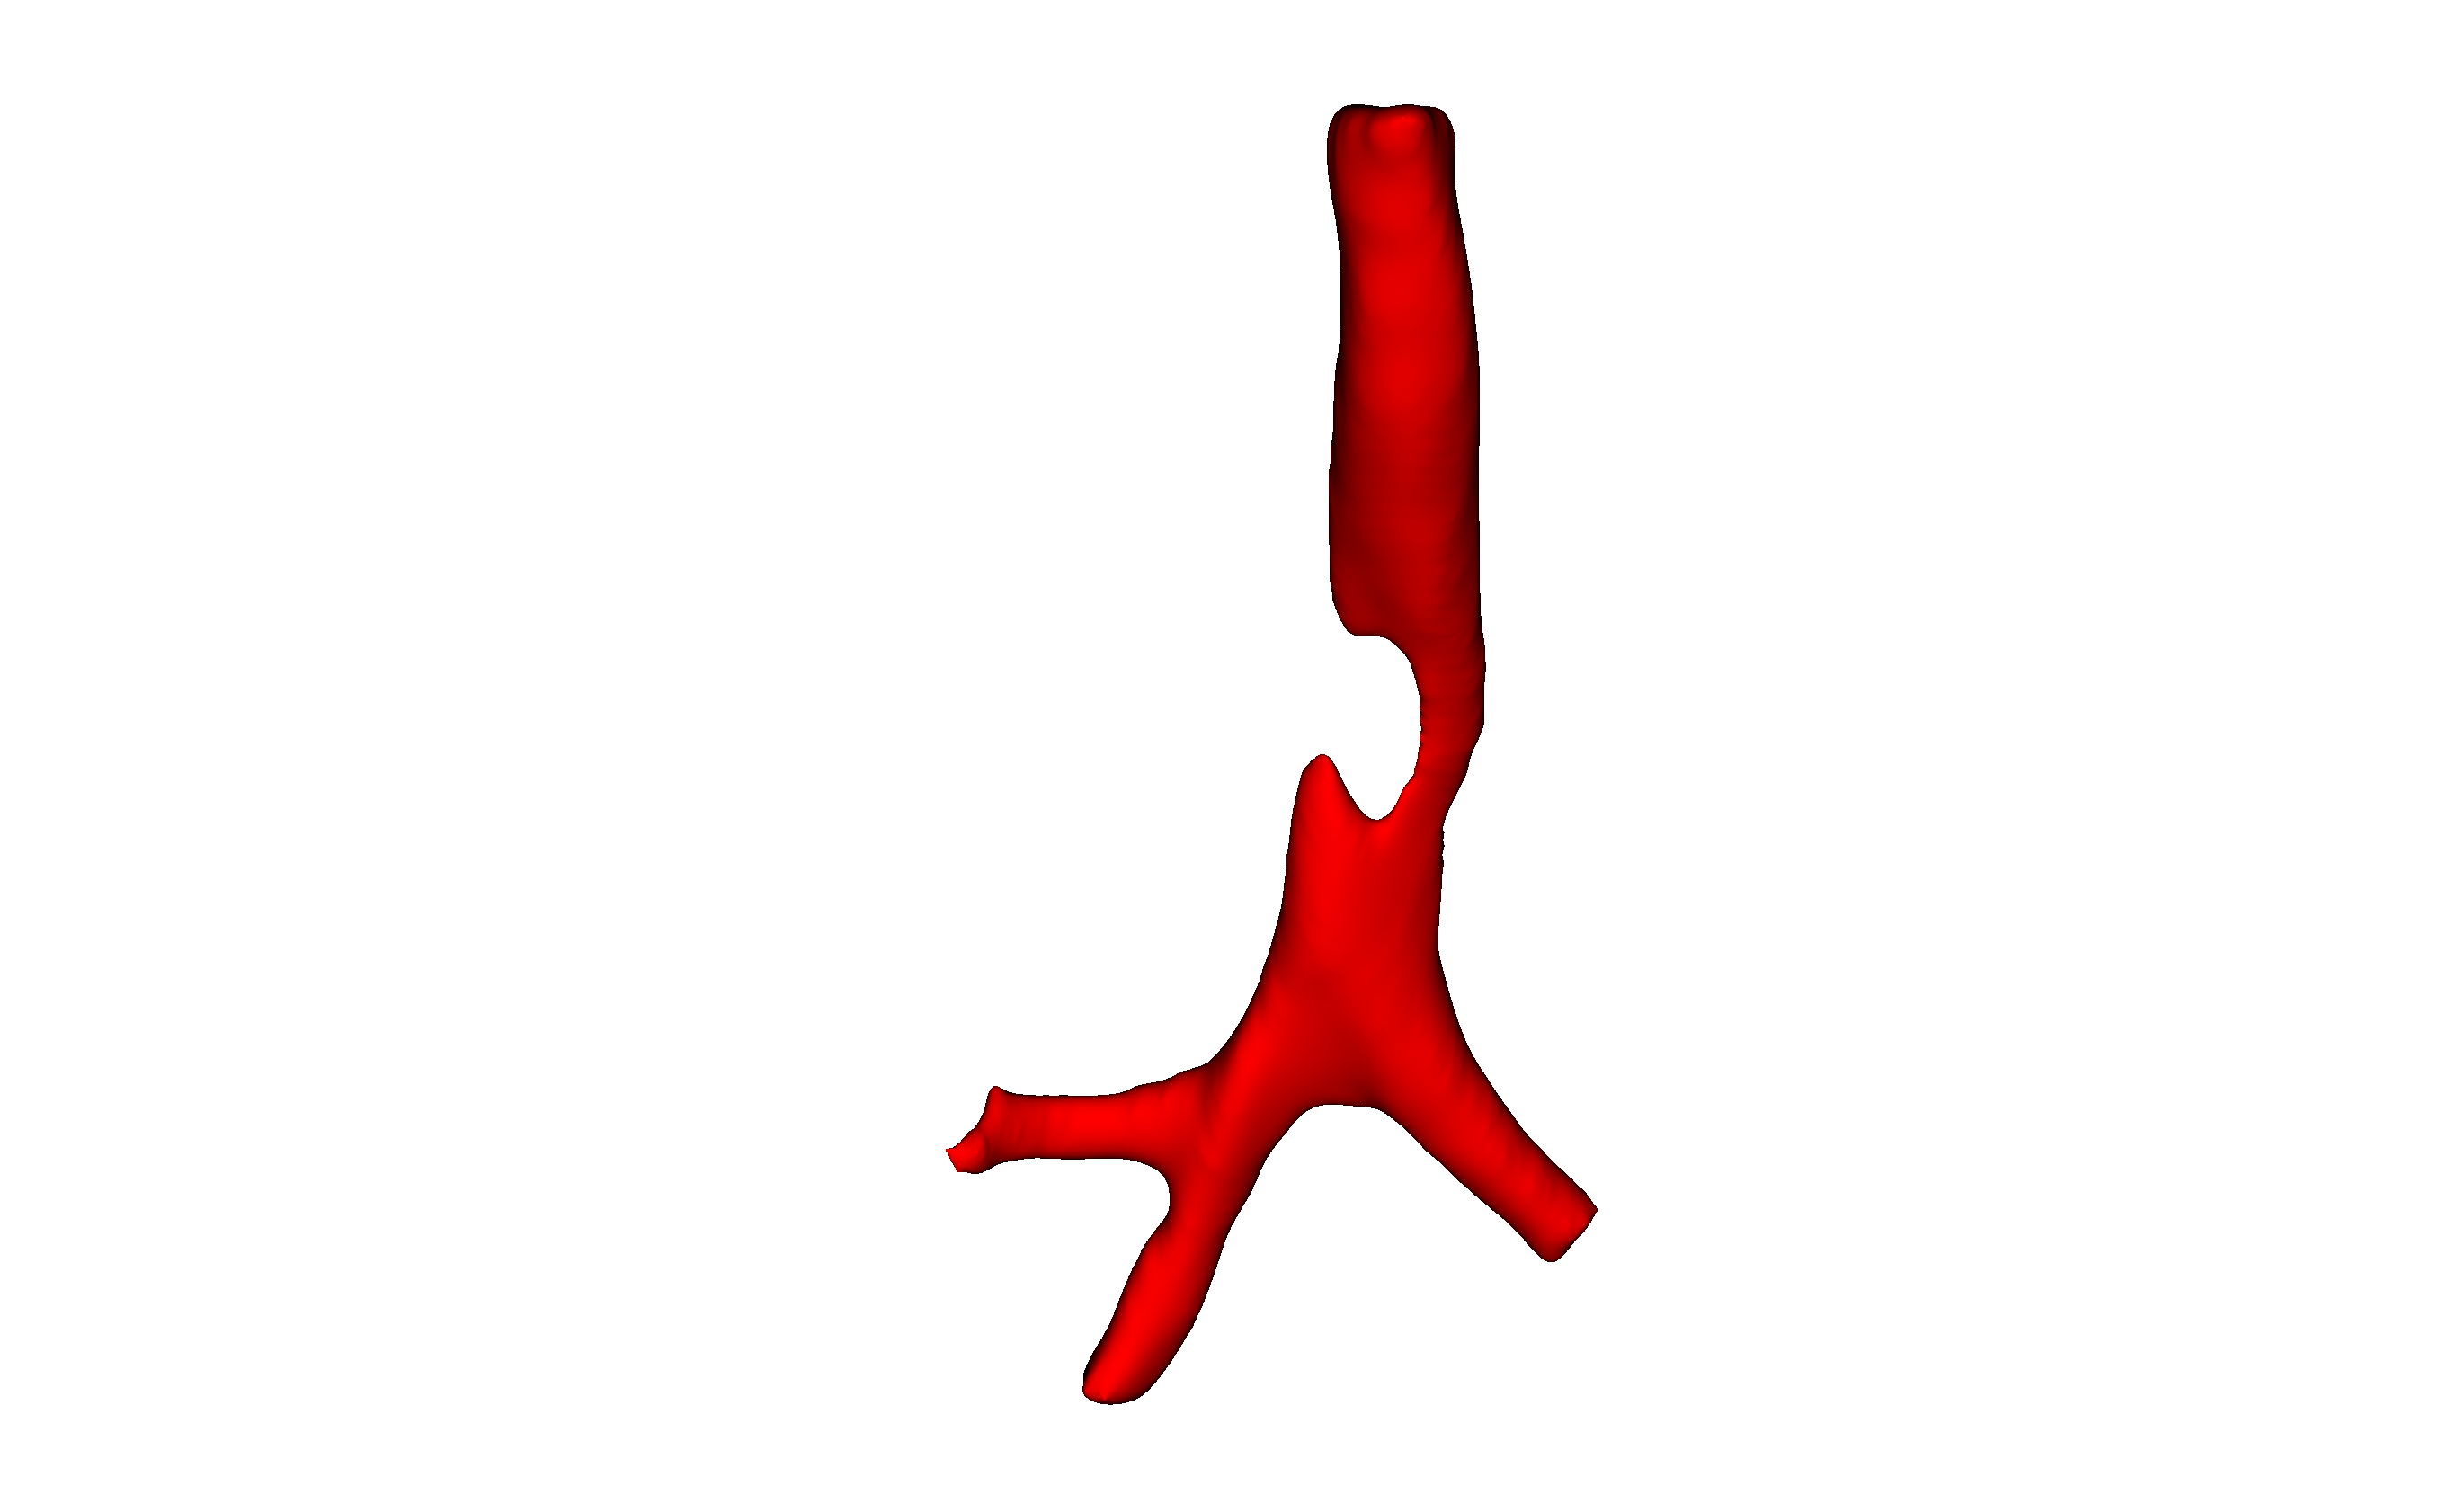
\includegraphics[width=\linewidth]{preop_segmentation.png}
    \caption{Preoperative cleaned airway segmentation.}
  \end{subfigure}\hfill
  \begin{subfigure}[t]{0.48\textwidth}
    \centering
    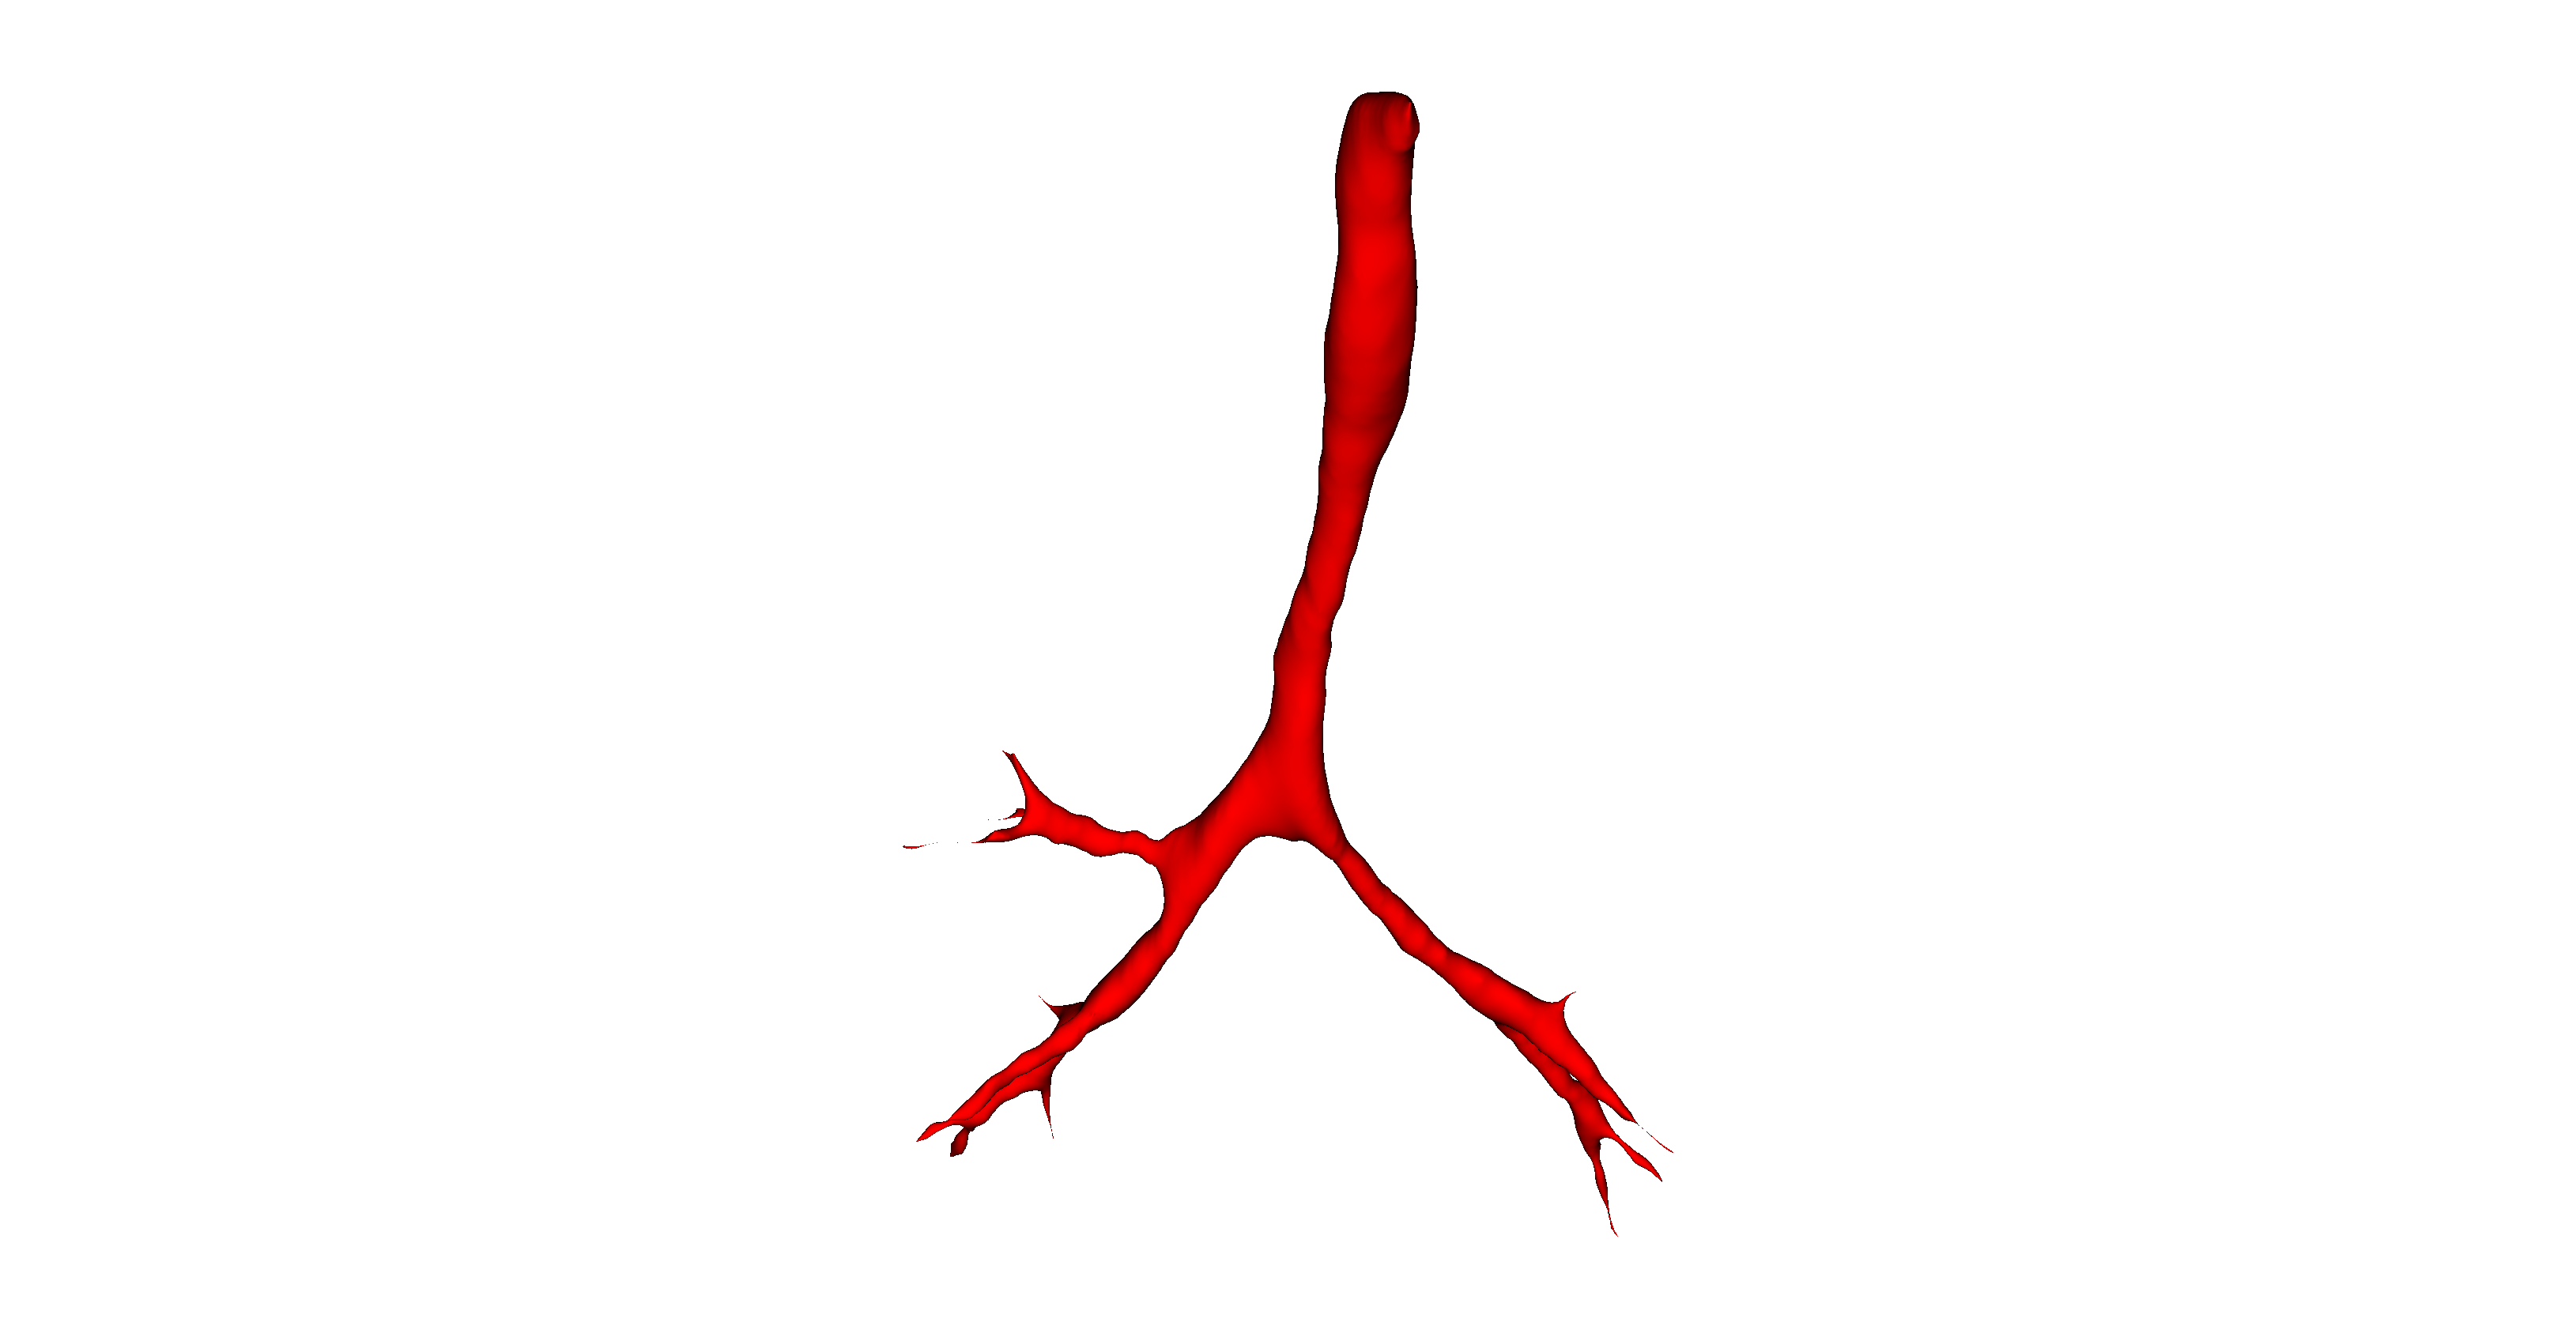
\includegraphics[width=\linewidth]{postop_segmentation.png}
    \caption{Postoperative airway segmentation.}
  \end{subfigure}

  \vspace{0.5em}
  \begin{subfigure}[t]{0.48\textwidth}
    \centering
    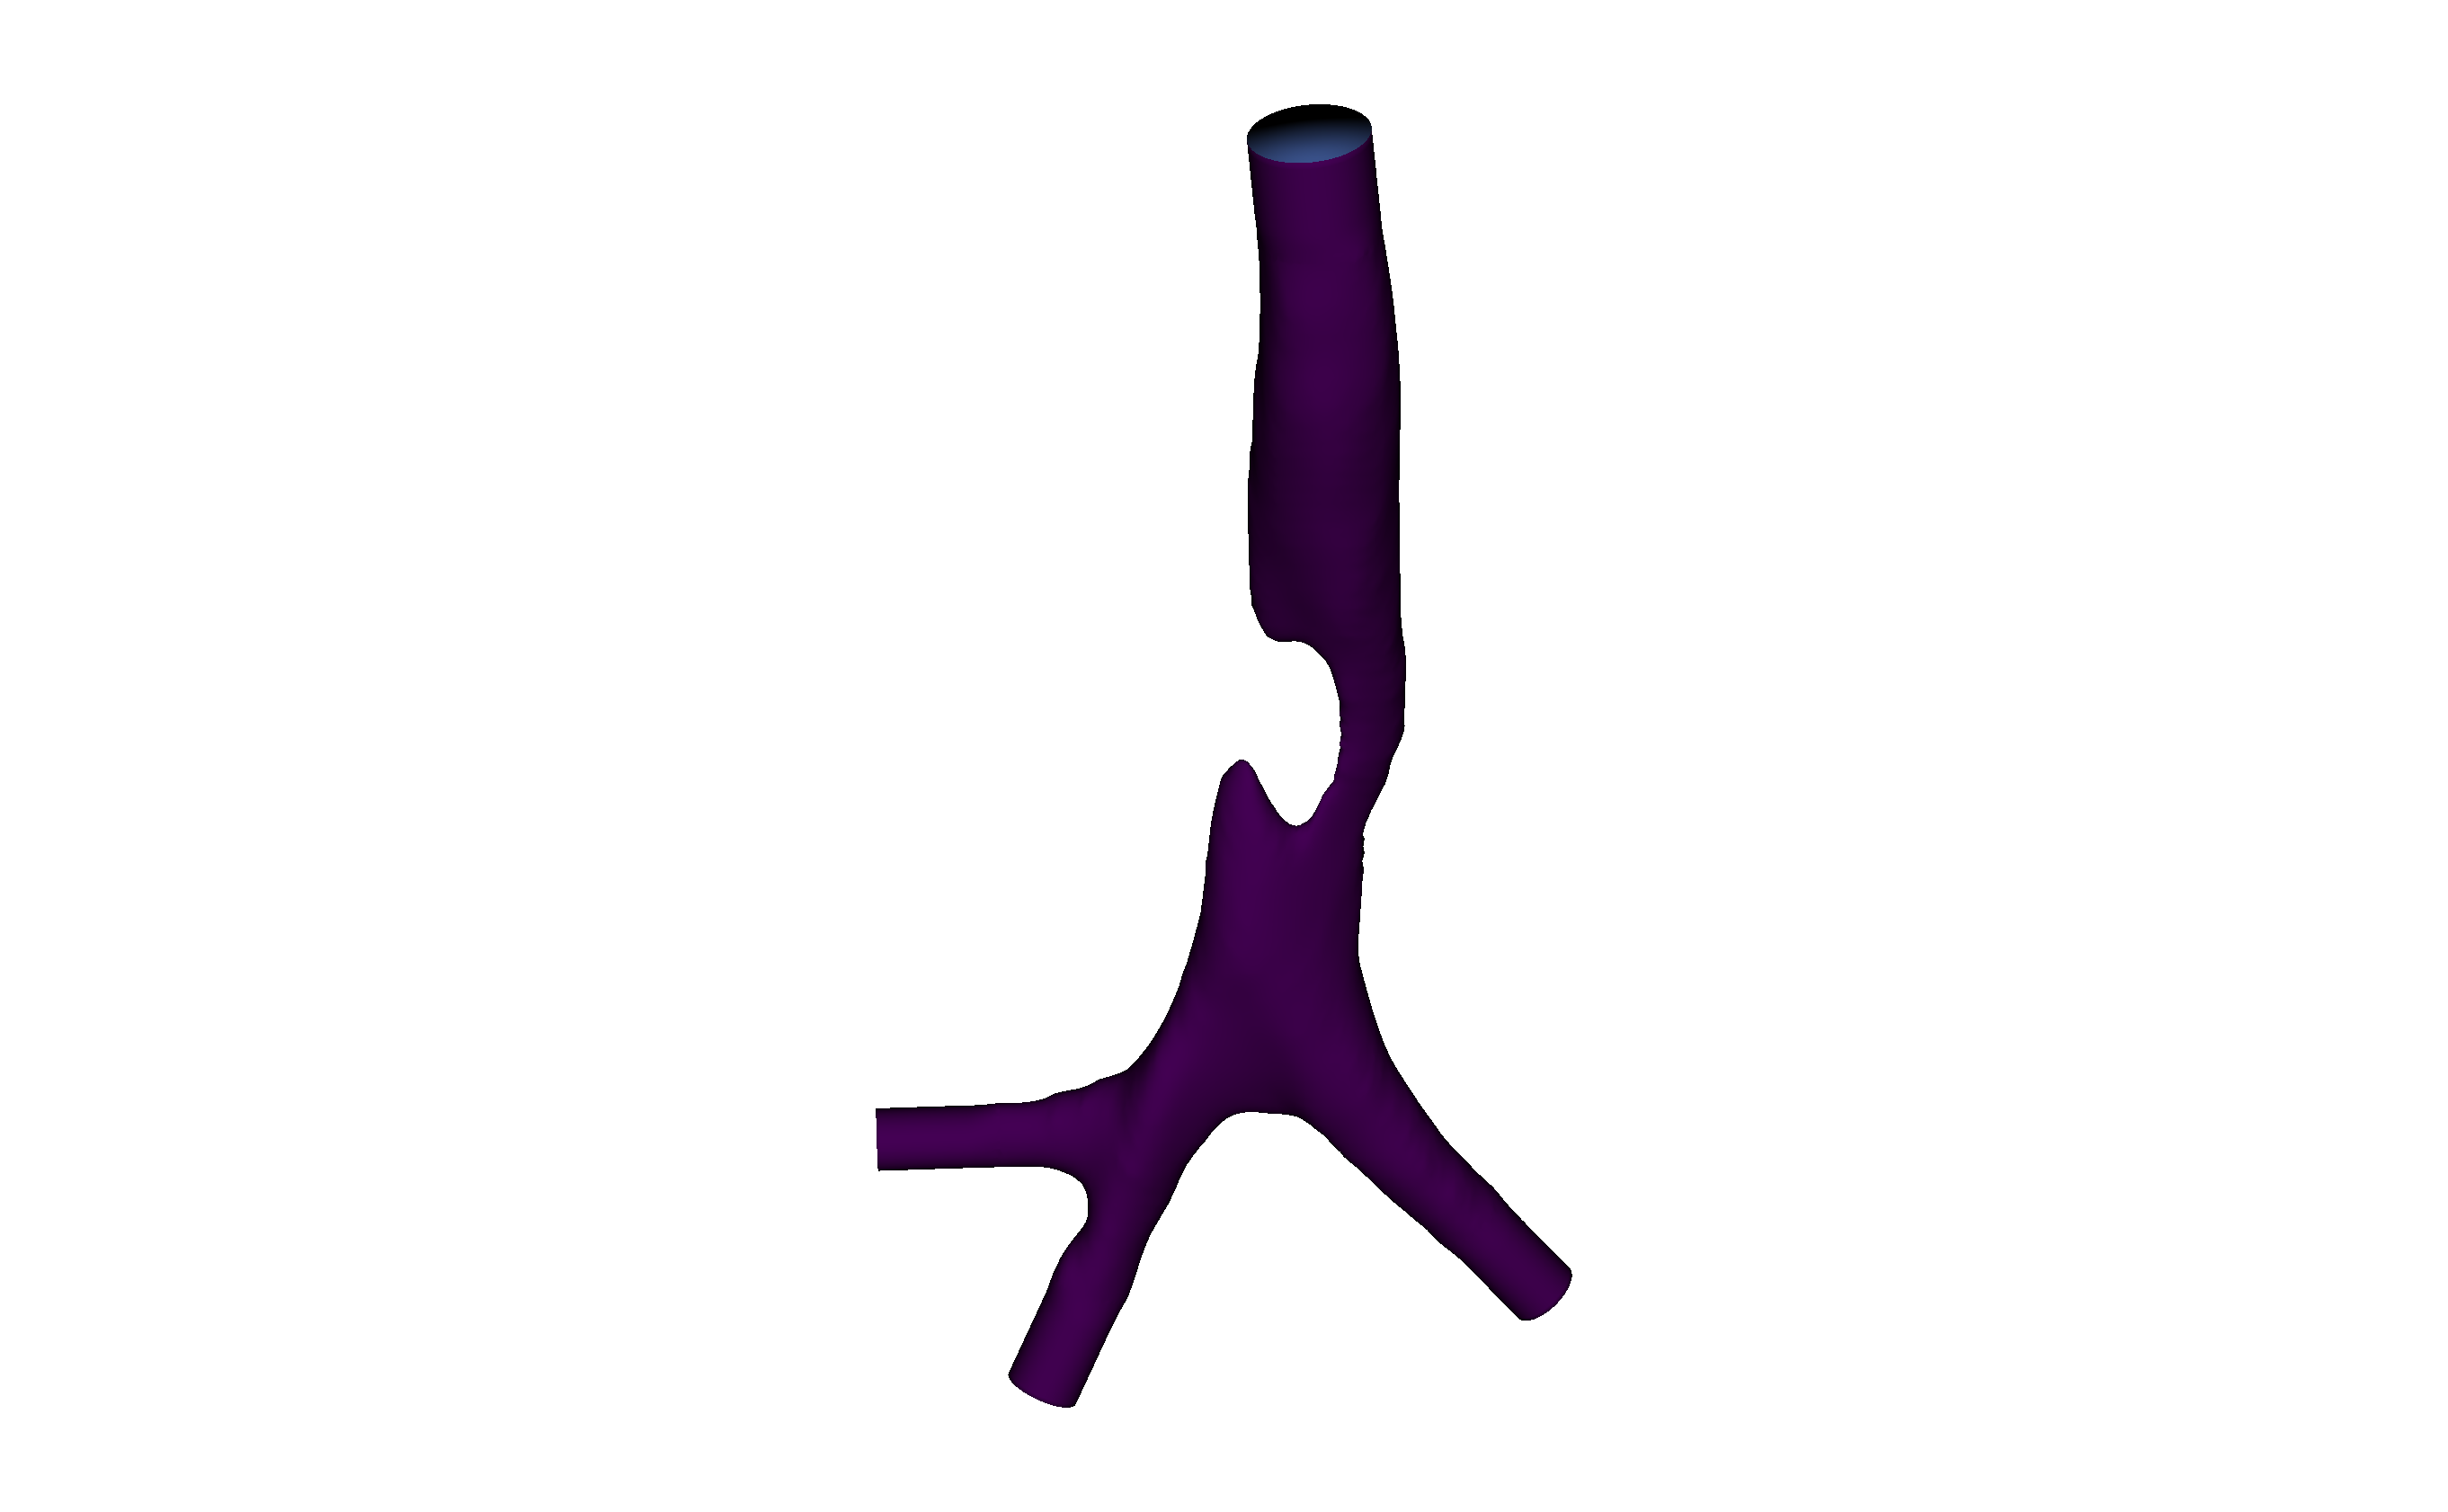
\includegraphics[width=\linewidth]{preop_cfd_surface.png}
    \caption{Preoperative clipped, extended, and capped surface.}
  \end{subfigure}\hfill
  \begin{subfigure}[t]{0.48\textwidth}
    \centering
    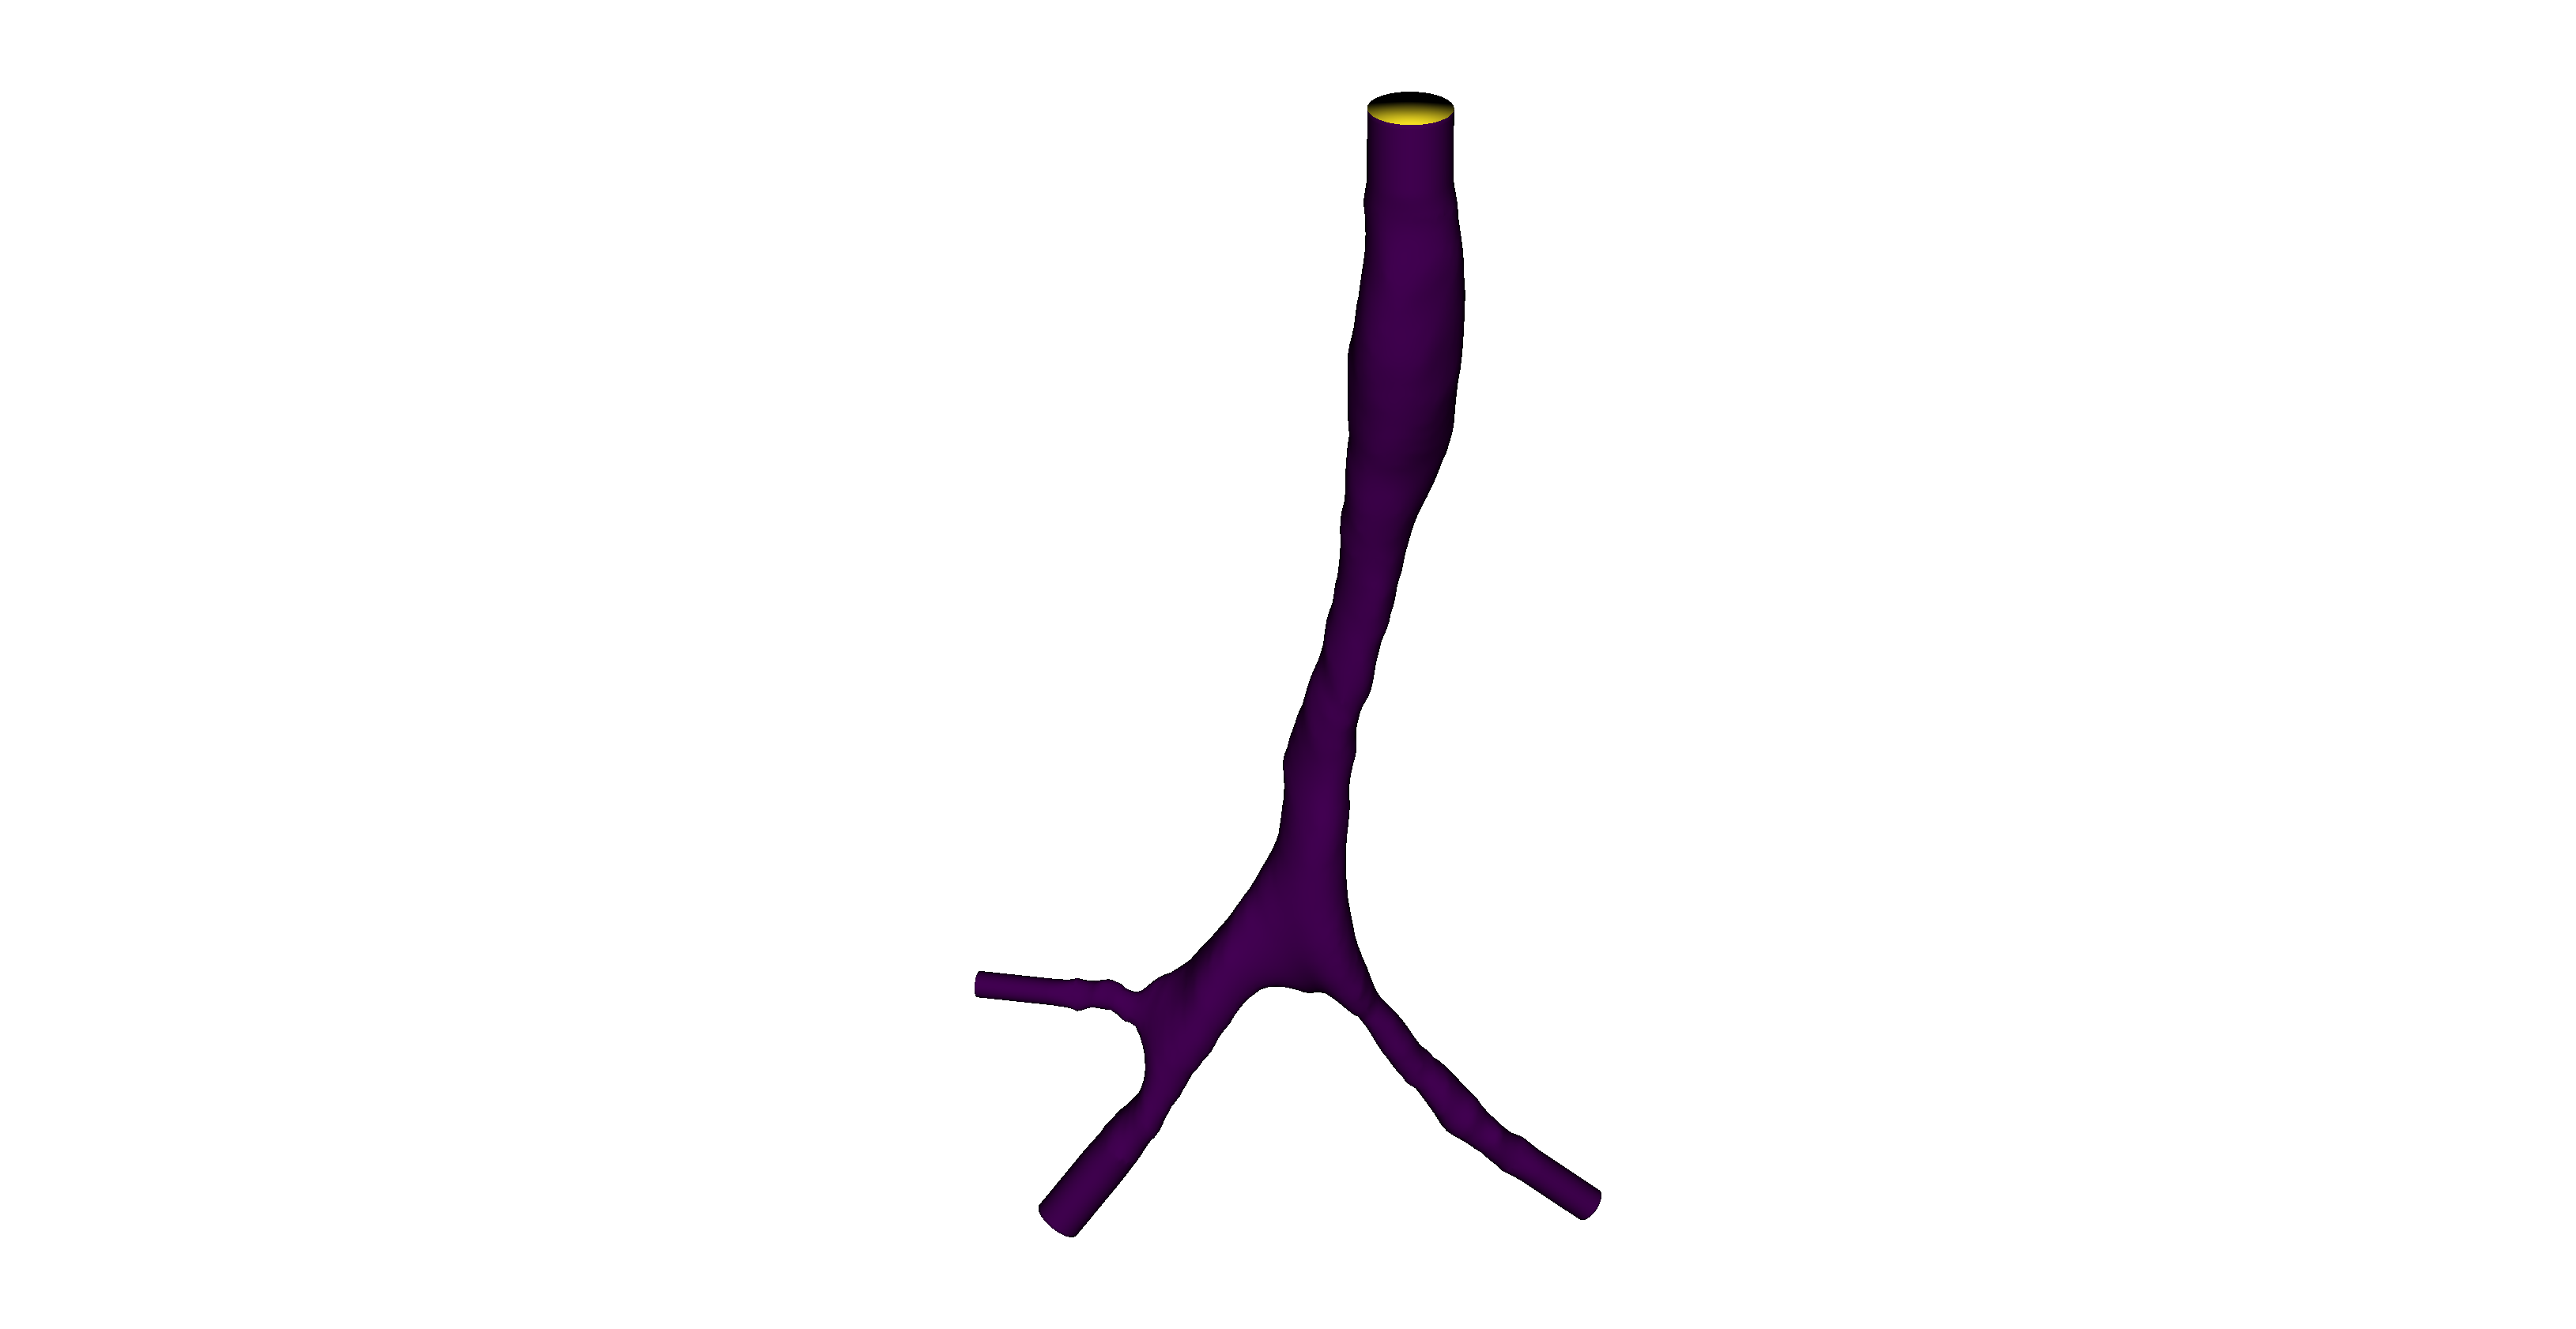
\includegraphics[width=\linewidth]{postop_cfd_surface.png}
    \caption{Postoperative clipped, extended, and capped surface.}
  \end{subfigure}
  \caption{Case-specific airway preparation in anatomical frontal view. The top
  row shows the live Slicer segmentations; the bottom row shows the final CFD
  surfaces with centerline-directed flow extensions and planar caps.}
  \label{fig:segmentation}
\end{figure}

\subsection{Anatomical measurements and degree of constriction}
\label{sec:anatomical_measurements}

The preoperative constriction is bounded by proximal and distal landmarks on the
tracheal centerline. Its length is measured along that centerline. Cross-sections
normal to the local centerline are sampled through the narrowed region to locate
the minimum lumen area. Because the lumen need not be circular, an equivalent
circular diameter is calculated from section area $A$ as

\begin{equation}
  D_{\mathrm{eq}} = 2\sqrt{\frac{A}{\pi}}.
\end{equation}

The postoperative area and equivalent diameter are measured using the same
procedure at 76.53\% of the inlet-to-carina centerline length. The carina is
defined from the airway-network bifurcation nearest the airway seed. The primary
area-based degree of constriction is

\begin{equation}
  C_A = \left(1-\frac{A_{\mathrm{pre,min}}}
  {A_{\mathrm{post,matched}}}\right)\times 100\%.
  \label{eq:area_constriction}
\end{equation}

The measured area constriction is 64.9\%. For transparency, the corresponding
minimum-Feret-diameter reduction is 65.2\% and is reported as

\begin{equation}
  C_D = \left(1-\frac{D_{\mathrm{pre,min}}}
  {D_{\mathrm{post,matched}}}\right)\times 100\%.
\end{equation}

\begin{table}[htbp]
  \centering
  \caption{Anatomical measurements obtained from centerline-normal lumen
  sections in 3D Slicer.}
  \label{tab:anatomical_measurements}
  \begin{tabular}{@{}lll@{}}
    \toprule
    Quantity & Symbol & Value \\
    \midrule
    Preoperative constriction length & $L_{\mathrm{pre}}$ & 12.157 \si{\milli\metre} \\
    Preoperative minimum area & $A_{\mathrm{pre,min}}$ & 1.813 \si{\milli\metre\squared} \\
    Preoperative minimum Feret diameter & $D_{\mathrm{pre,Feret}}$ & 0.798 \si{\milli\metre} \\
    Preoperative equivalent diameter & $D_{\mathrm{pre,eq}}$ & 1.519 \si{\milli\metre} \\
    Postoperative matched area & $A_{\mathrm{post,matched}}$ & 5.169 \si{\milli\metre\squared} \\
    Postoperative minimum Feret diameter & $D_{\mathrm{post,Feret}}$ & 2.292 \si{\milli\metre} \\
    Postoperative equivalent diameter & $D_{\mathrm{post,eq}}$ & 2.565 \si{\milli\metre} \\
    Area constriction & $C_A$ & 64.9\% \\
    Minimum Feret diameter reduction & $C_{D,\mathrm{Feret}}$ & 65.2\% \\
    \bottomrule
  \end{tabular}
\end{table}

The measured dimensions are consistent with the scale reported in paediatric
tracheal-surgery literature. Arcieri et al. described 25 children with congenital
tracheal stenosis and reported a mean internal diameter of
\SI{1.5}{\milli\metre}; the cohort had a median operative age of seven months and
median weight of \SI{5.2}{\kilogram} \cite{arcieri2018}. This closely matches the
\SI{1.519}{\milli\metre} preoperative equivalent diameter obtained here. The
smaller minimum Feret diameter of \SI{0.798}{\milli\metre} is not contradictory:
it characterises the narrowest caliper dimension of a non-circular lumen, whereas
the equivalent diameter is derived from total cross-sectional area. The
literature comparison supports dimensional plausibility but is not an independent
validation of the patient-specific segmentation or landmark placement.

\begin{figure}[htbp]
  \centering
  \begin{subfigure}[t]{0.48\textwidth}
    \centering
    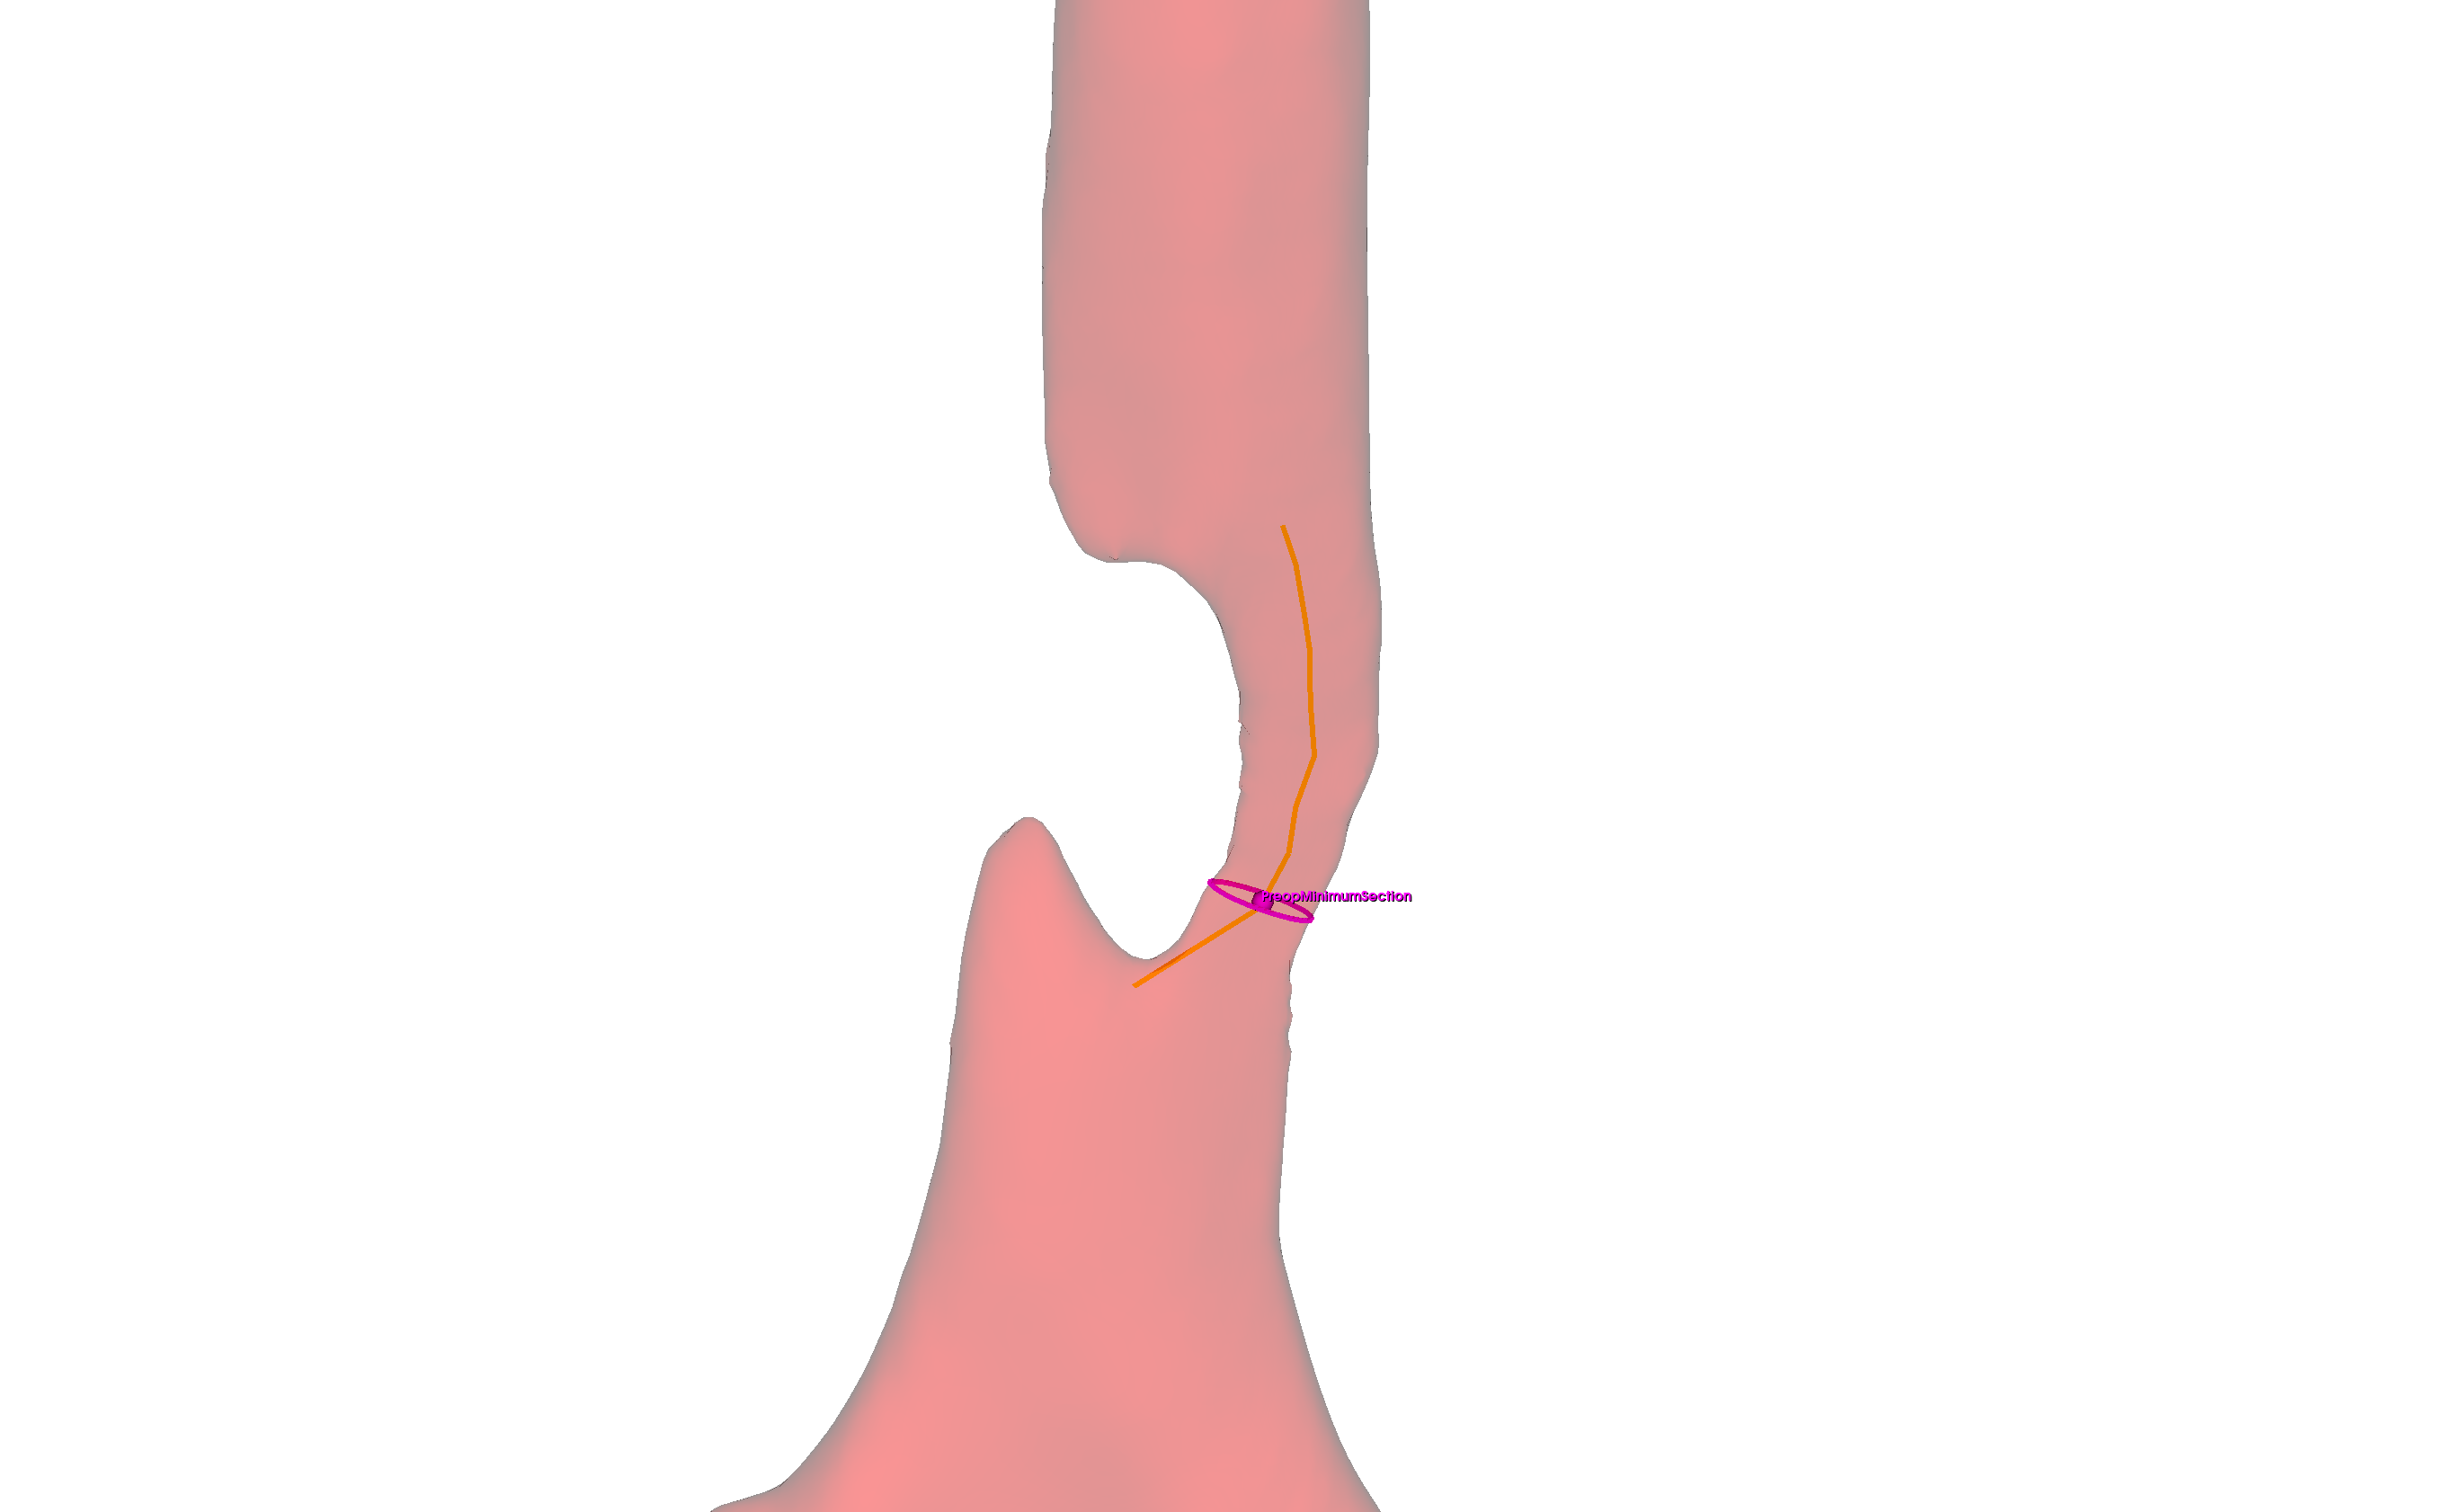
\includegraphics[width=\linewidth]{preop_stenosis_measurement.png}
    \caption{Preoperative stenosis path and minimum section.}
  \end{subfigure}\hfill
  \begin{subfigure}[t]{0.48\textwidth}
    \centering
    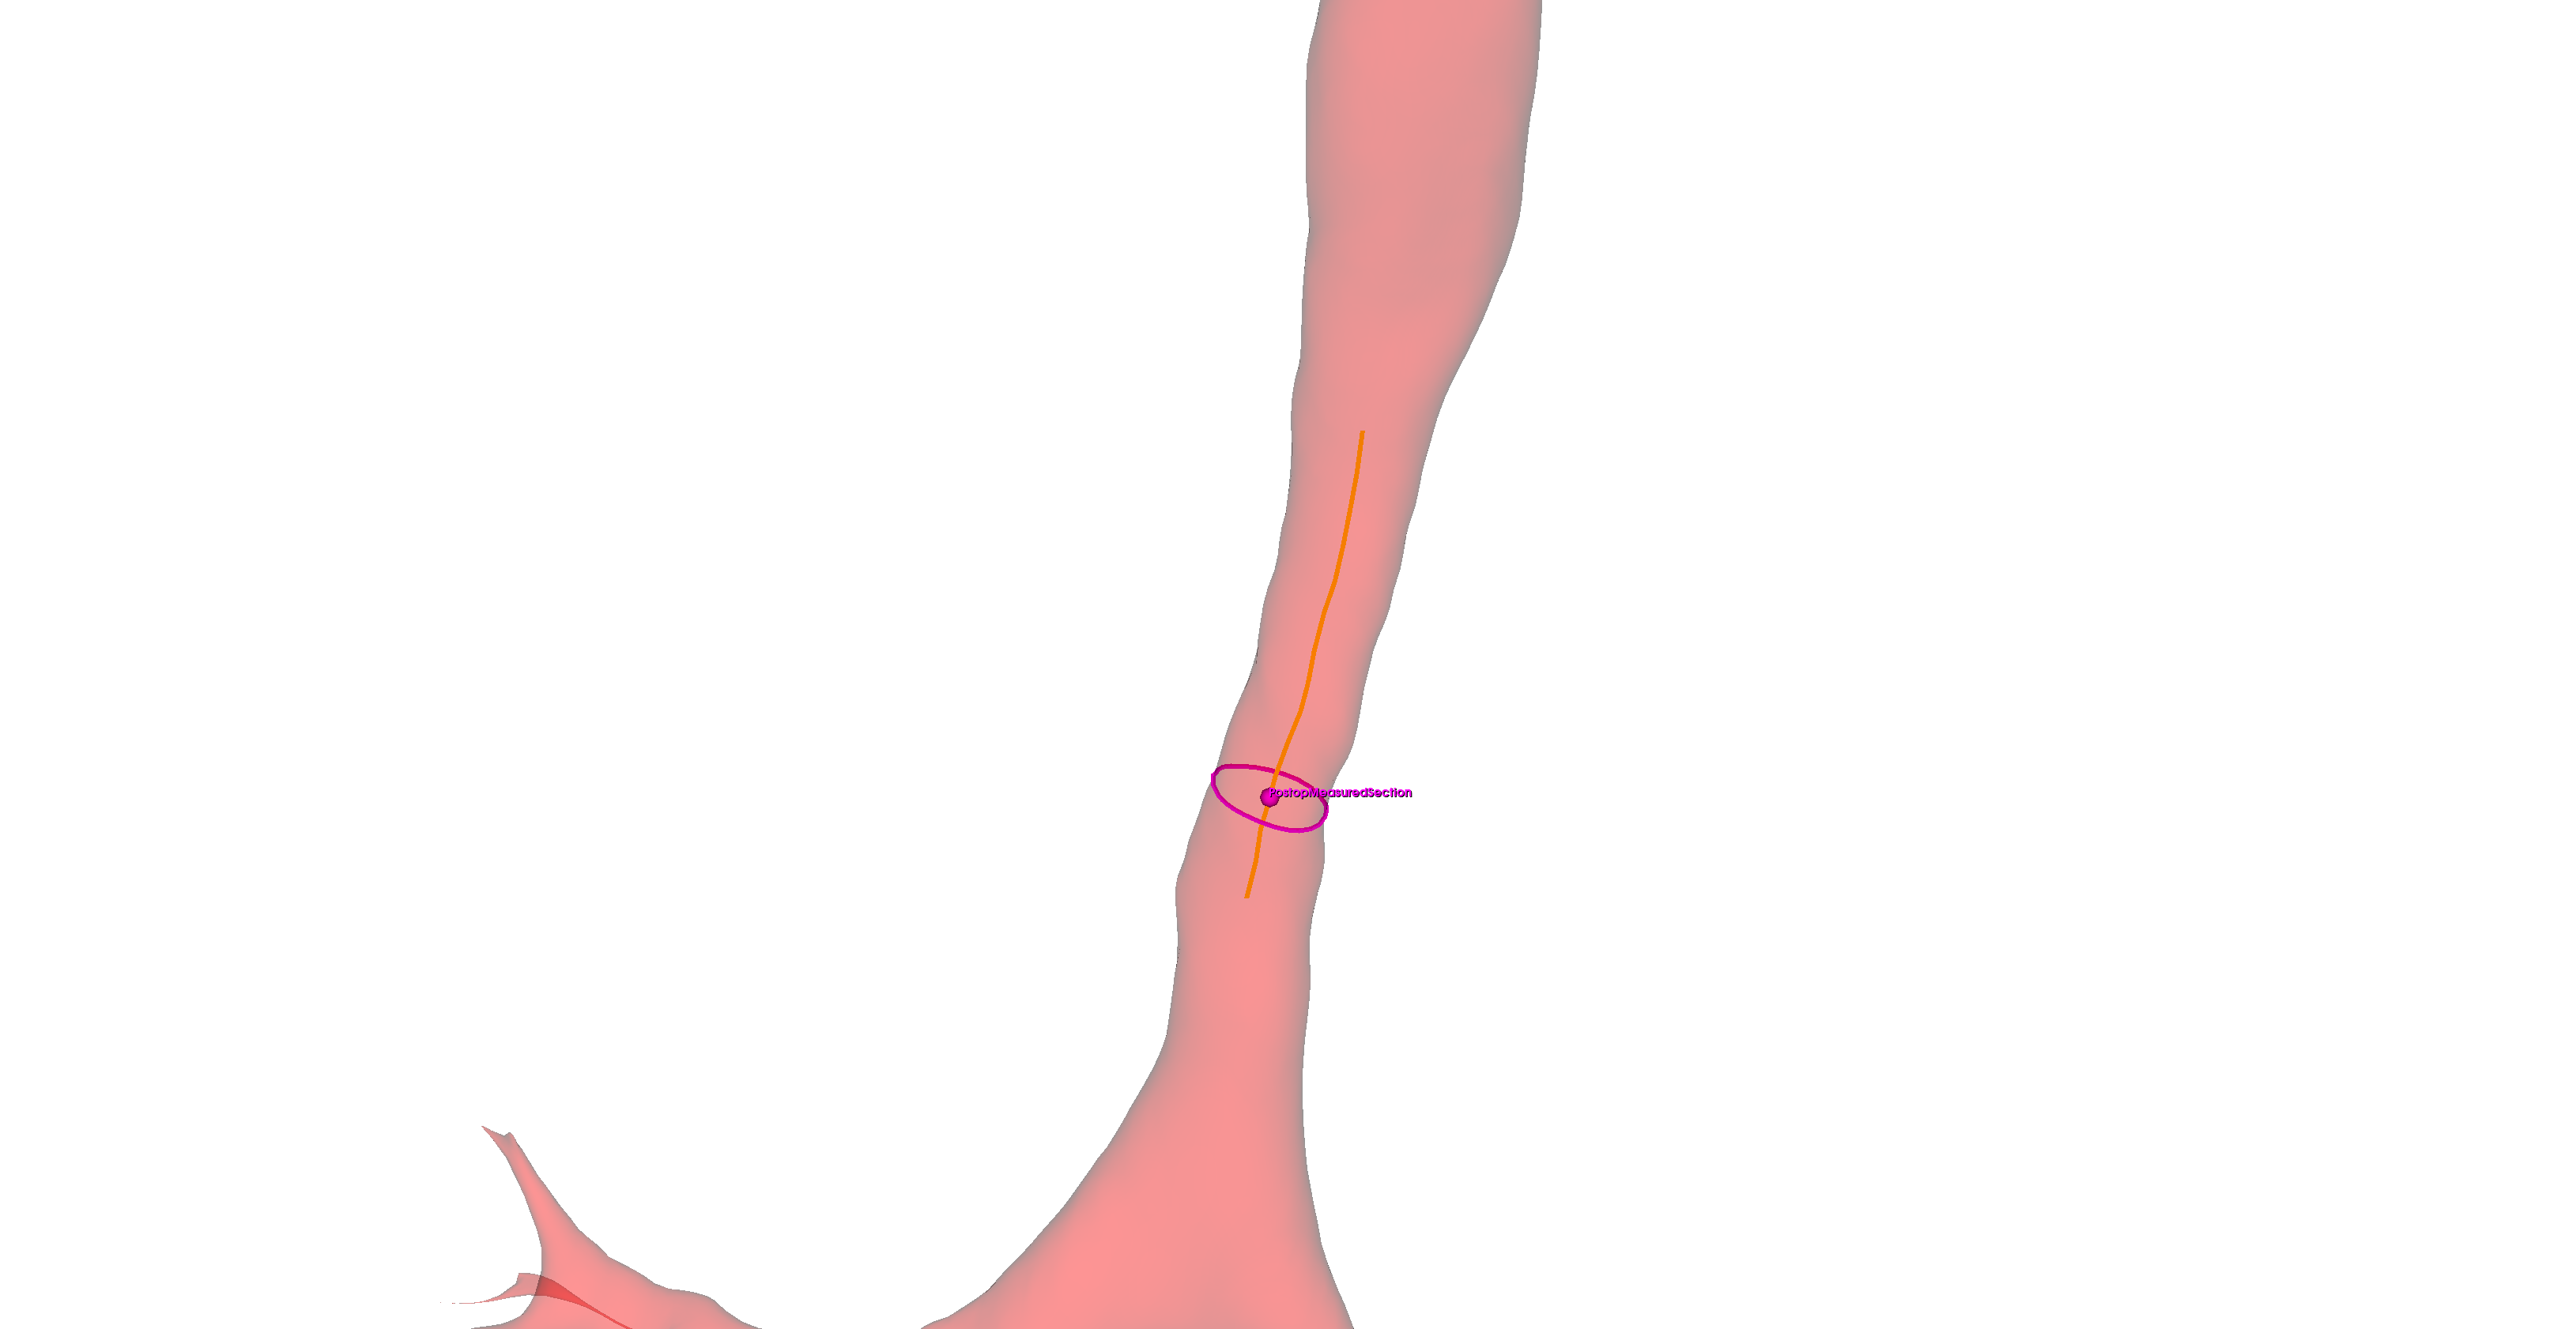
\includegraphics[width=\linewidth]{postop_matched_section.png}
    \caption{Mapped postoperative comparison section.}
  \end{subfigure}
  \caption{Centerline-based anatomical correspondence. Orange curves show the
  measured tracheal interval and magenta contours identify the preoperative
  minimum and corresponding postoperative lumen sections. The postoperative
  location is mapped using 76.53\% of inlet-to-carina centerline distance.}
  \label{fig:anatomical_measurements}
\end{figure}

\subsection{Qualitative flow behaviour through the constriction}

For incompressible flow, continuity $Q=AU$ requires velocity to rise as the area
narrows and fall after expansion. Before the stenosis, pressure decreases
gradually because viscous wall shear opposes motion; for laminar circular flow,
$\Delta p=128\mu LQ/(\pi D^4)$. Through the stenosis, acceleration converts
static pressure into kinetic energy according to Bernoulli's principle, while
viscosity and separation add irreversible loss. Downstream, deceleration causes
partial pressure recovery, but pressure remains below the upstream trend because
separation, mixing, and wall friction dissipate mechanical energy.

\begin{figure}[htbp]
  \centering
  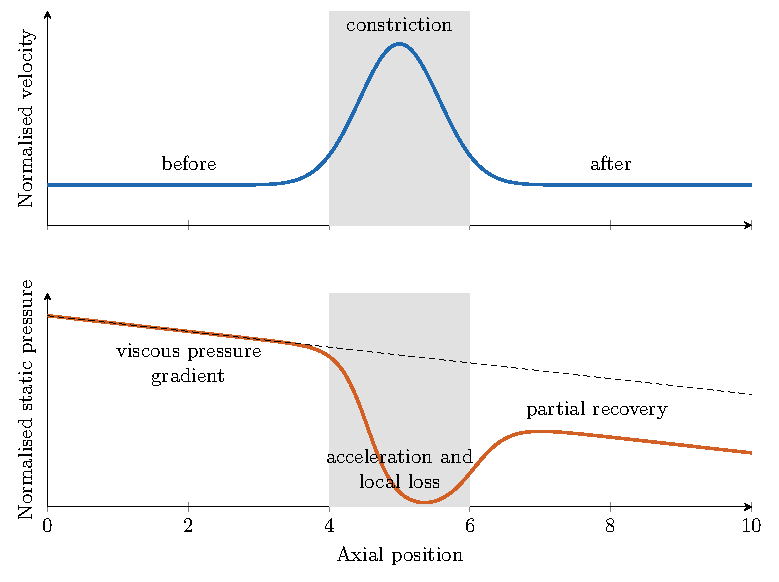
\includegraphics[width=0.88\textwidth]{assignment3_flow_behavior.pdf}
  \caption{Qualitative velocity and static-pressure evolution through a
  constriction. Velocity increases as area decreases; pressure falls sharply
  through the stenosis and recovers only partially downstream. Curves are
  schematic and not CFD results.}
  \label{fig:assignment3_flow_behavior}
\end{figure}

% -----------------------------------------------------------------------------
\section{Volume mesh generation}
\label{sec:mesh}

The triangulated STL surface is imported into Gmsh. Surface classification and
geometry creation produce a closed fluid volume. The physical boundary groups
are:

\begin{itemize}
  \item \texttt{inlet}: tracheal inlet;
  \item \texttt{outlet\_1}: right superior lobar bronchus;
  \item \texttt{outlet\_2}: right inferior lobar bronchus;
  \item \texttt{outlet\_3}: left main bronchus;
  \item \texttt{wall}: remaining airway surface; and
  \item \texttt{fluid}: internal volume.
\end{itemize}

The physical groups are visually verified whenever the STL topology or Gmsh
classification changes. The volume consists of first-order tetrahedra with a
uniform target characteristic length controlled by \texttt{MESH\_SIZE}.

\begin{table}[htbp]
  \centering
  \caption{Replicable mesh settings and quality metrics. All current volume
  elements are first-order tetrahedra. Add the exact Gmsh version and final
  values from each \texttt{checkMesh} log.}
  \label{tab:meshes}
  \resizebox{\textwidth}{!}{%
  \begin{tabular}{@{}lrrrrrr@{}}
    \toprule
    Mesh & Target size (mm) & Points & Cells & Element type & Max. aspect ratio & Max. non-orthogonality \\
    \midrule
    HXT baseline & 0.25 & 39,977  & 180,163   & Tetrahedron & 114.14 & 88.63$^\circ$ \\
    HXT fine 1   & 0.20 & 71,198  & 339,886   & Tetrahedron & 11.73  & 80.29$^\circ$ \\
    HXT fine 2   & 0.15 & 151,599 & 776,568   & Tetrahedron & 12.63  & 69.82$^\circ$ \\
    HXT densest  & 0.12 & 281,330 & 1,493,440 & Tetrahedron & 88.00  & 82.34$^\circ$ \\
    \bottomrule
  \end{tabular}%
  }
\end{table}

\subsection{Near-wall resolution}

Boundary-layer prism elements are commonly used near no-slip walls because they
resolve steep wall-normal velocity gradients efficiently and with better cell
alignment than isotropic tetrahedra. The current Gmsh workflow uses only
first-order tetrahedra and does not include dedicated inflation layers. This
must not be presented as a hybrid boundary-layer mesh. Its consequences are
considered when interpreting wall-adjacent quantities, and adding prism layers
is identified as a model improvement.

The Gmsh mesh uses millimetres because it inherits the Slicer coordinate scale.
After \texttt{gmshToFoam}, all coordinates are multiplied by $10^{-3}$ to obtain
SI units.

\begin{figure}[htbp]
  \centering
  \begin{subfigure}[t]{0.48\textwidth}
    \centering
    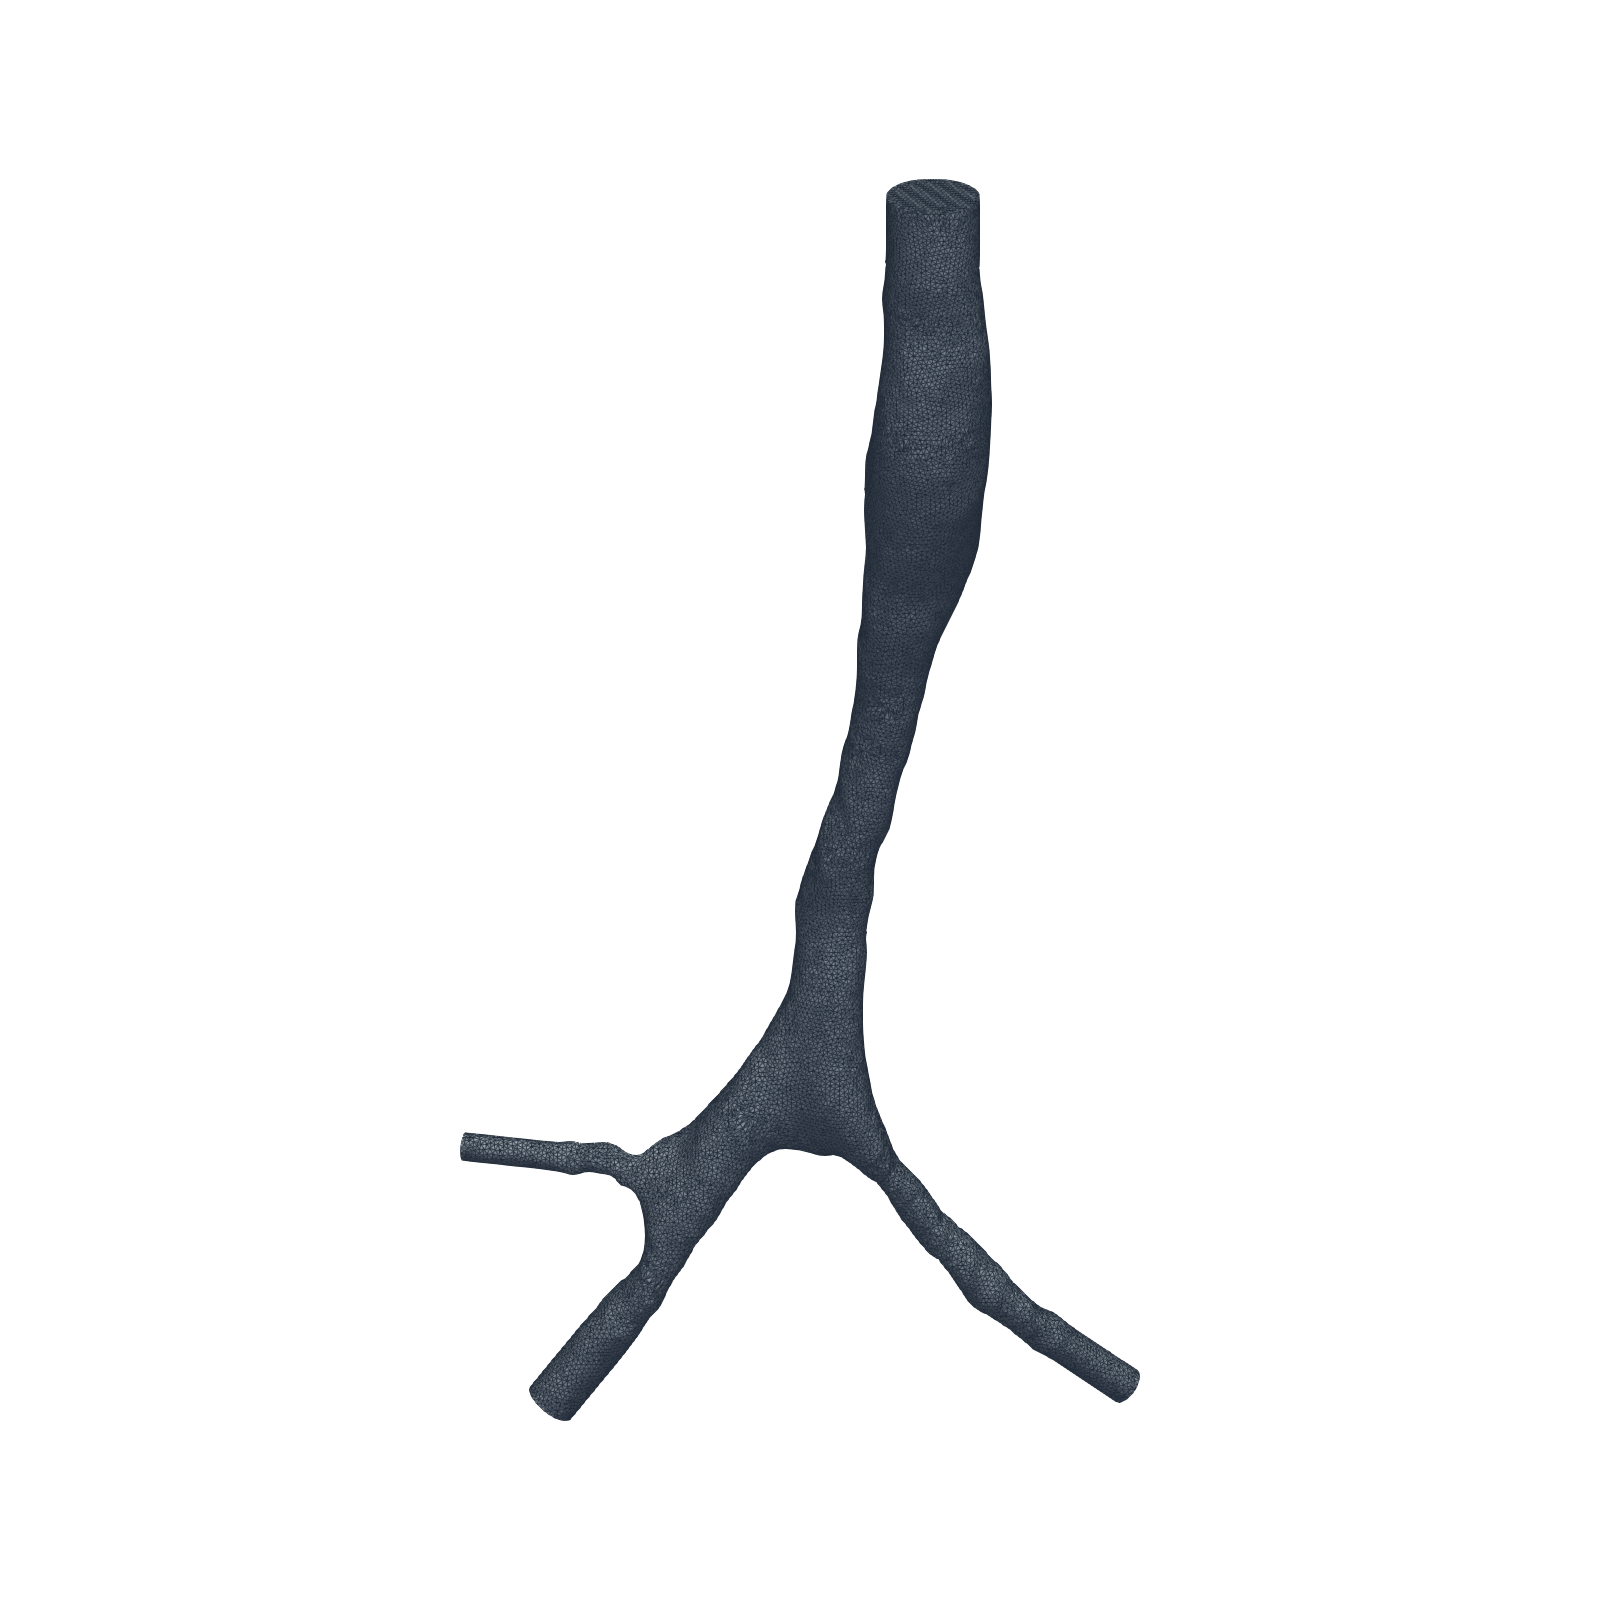
\includegraphics[width=\linewidth]{assignment5_mesh_025_full.png}
    \caption{0.25 mm HXT baseline; 180,163 volume cells.}
  \end{subfigure}\hfill
  \begin{subfigure}[t]{0.48\textwidth}
    \centering
    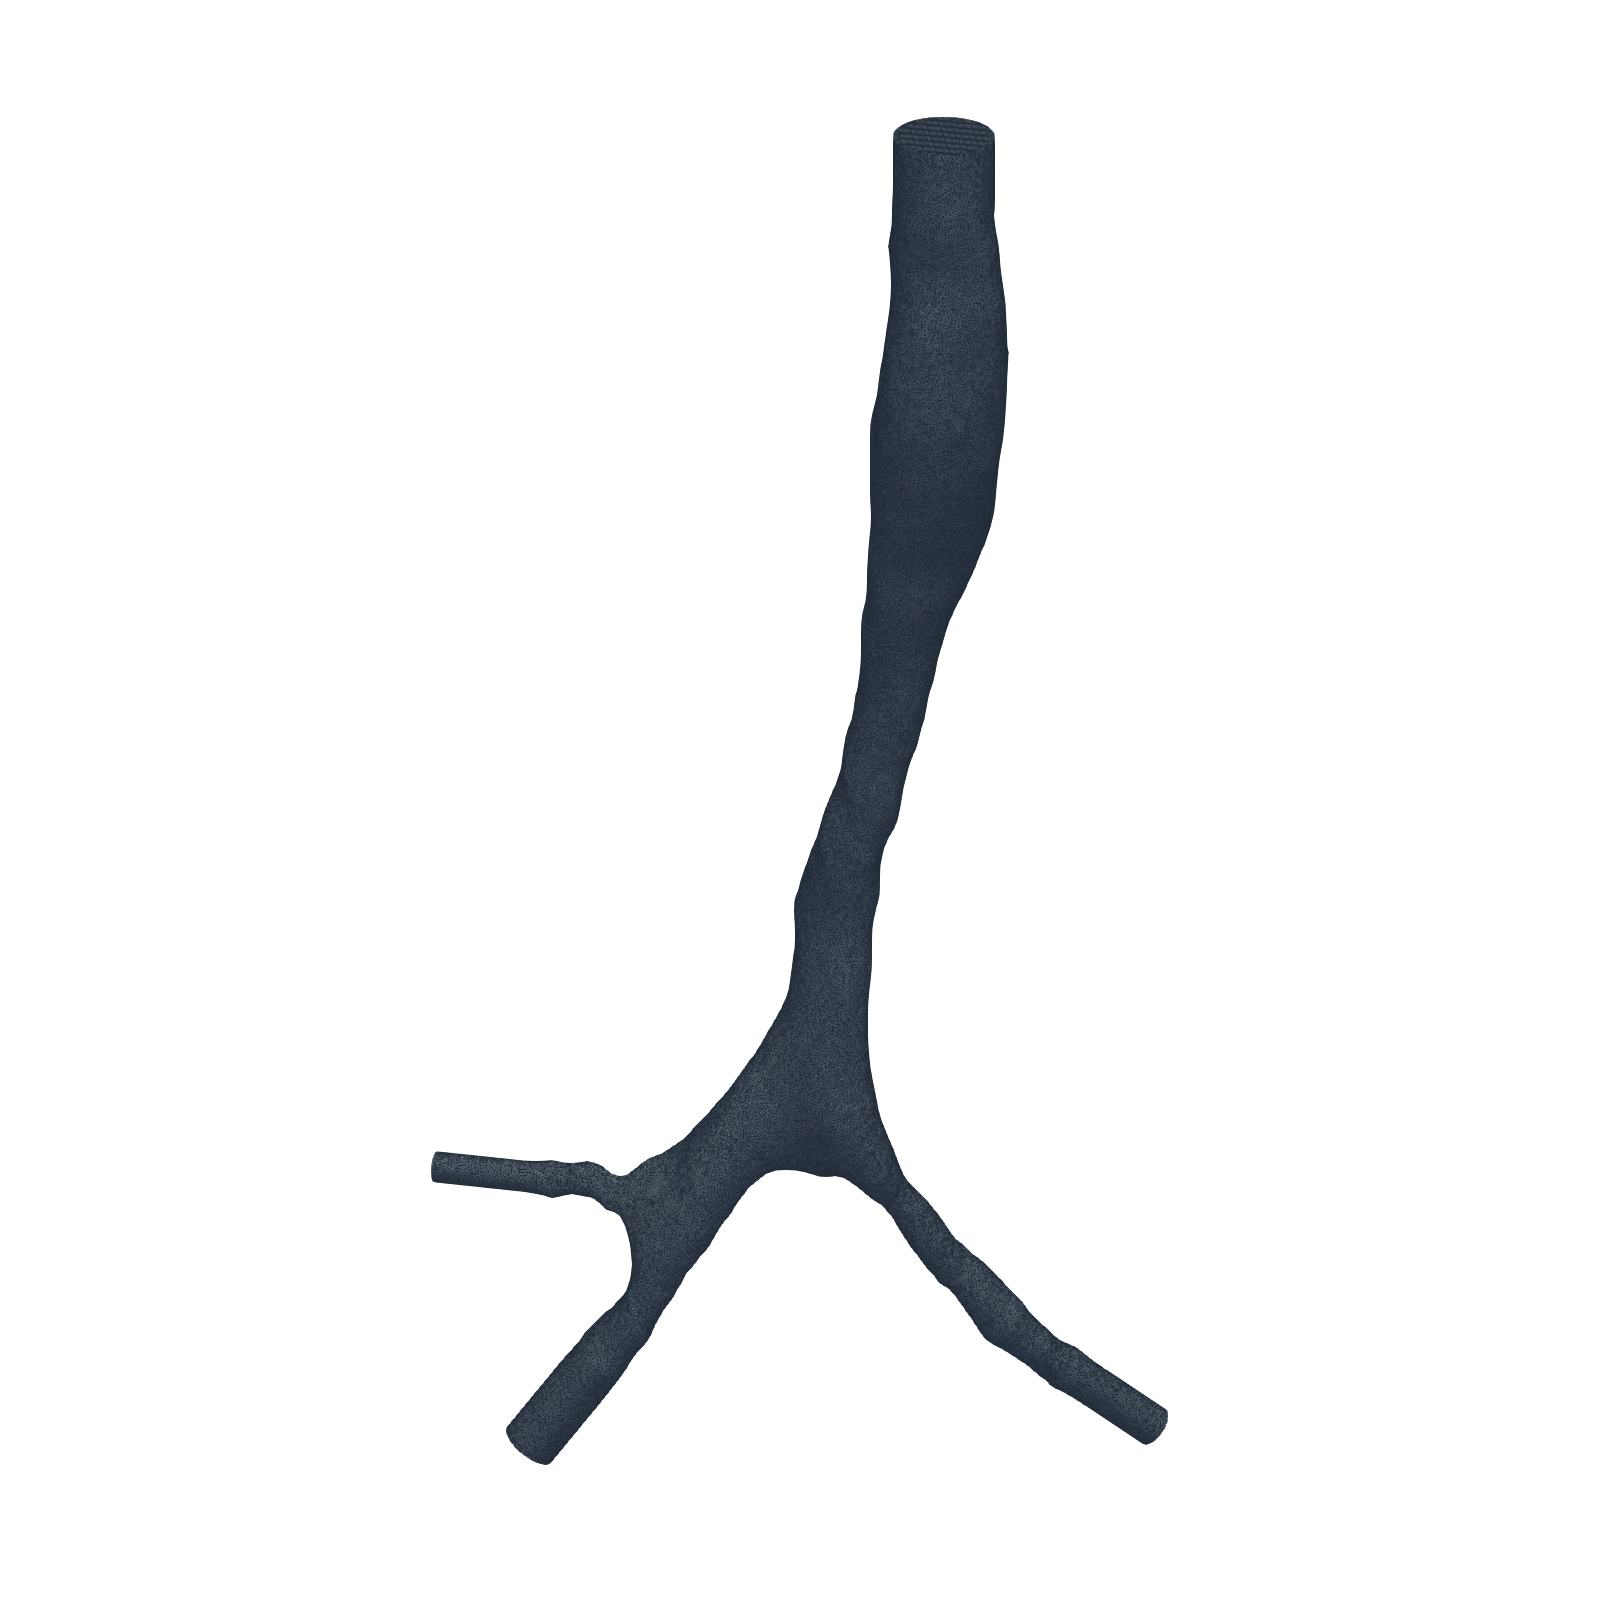
\includegraphics[width=\linewidth]{assignment5_mesh_015_full.png}
    \caption{Selected 0.15 mm HXT mesh; 776,568 volume cells.}
  \end{subfigure}

  \vspace{0.5em}
  \begin{subfigure}[t]{0.48\textwidth}
    \centering
    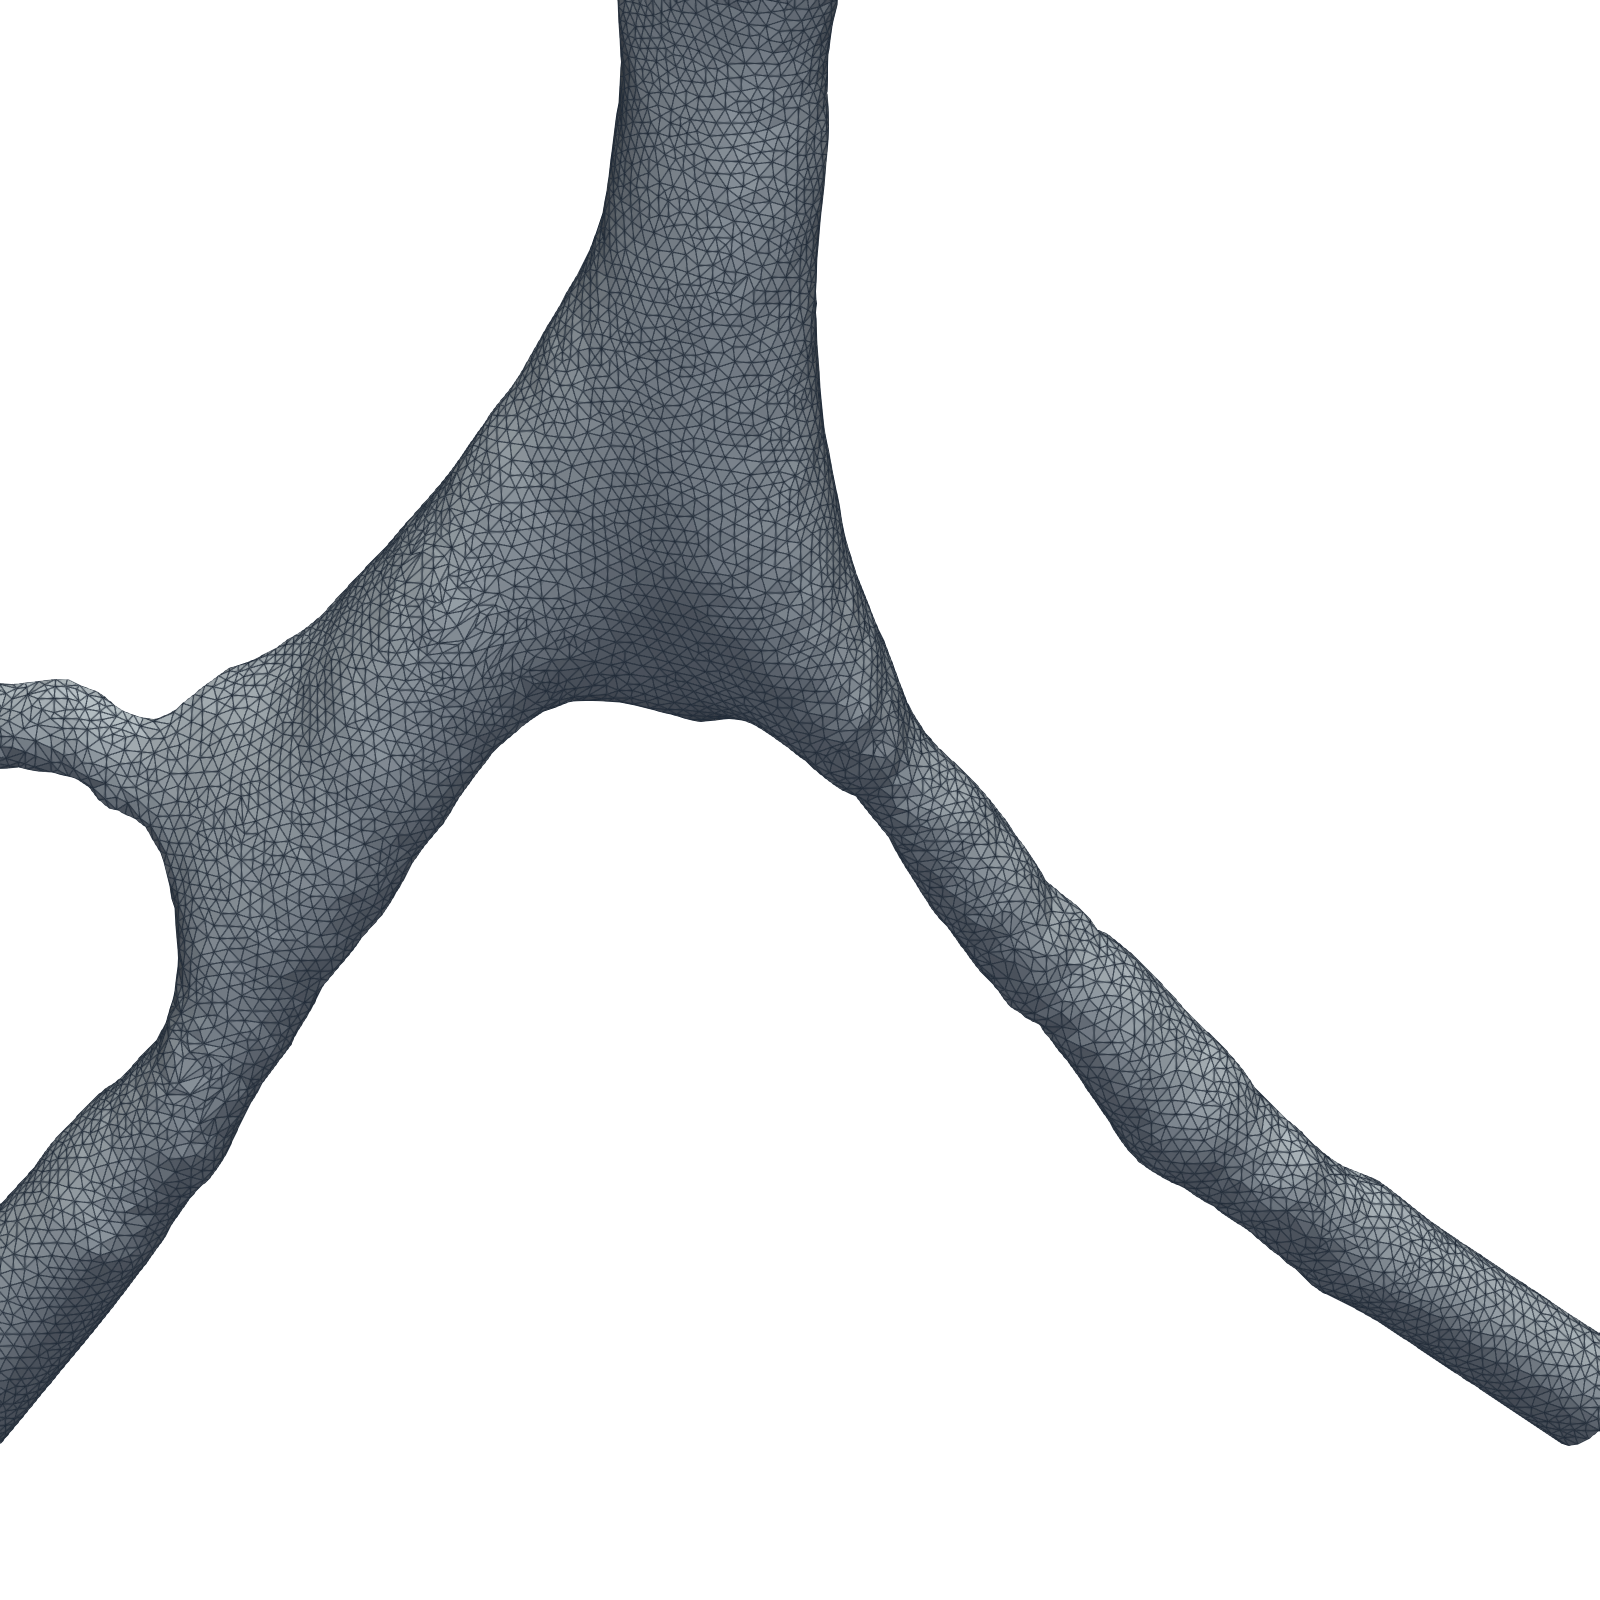
\includegraphics[width=\linewidth]{assignment5_mesh_025_closeup.png}
    \caption{Baseline surface triangulation at the carina.}
  \end{subfigure}\hfill
  \begin{subfigure}[t]{0.48\textwidth}
    \centering
    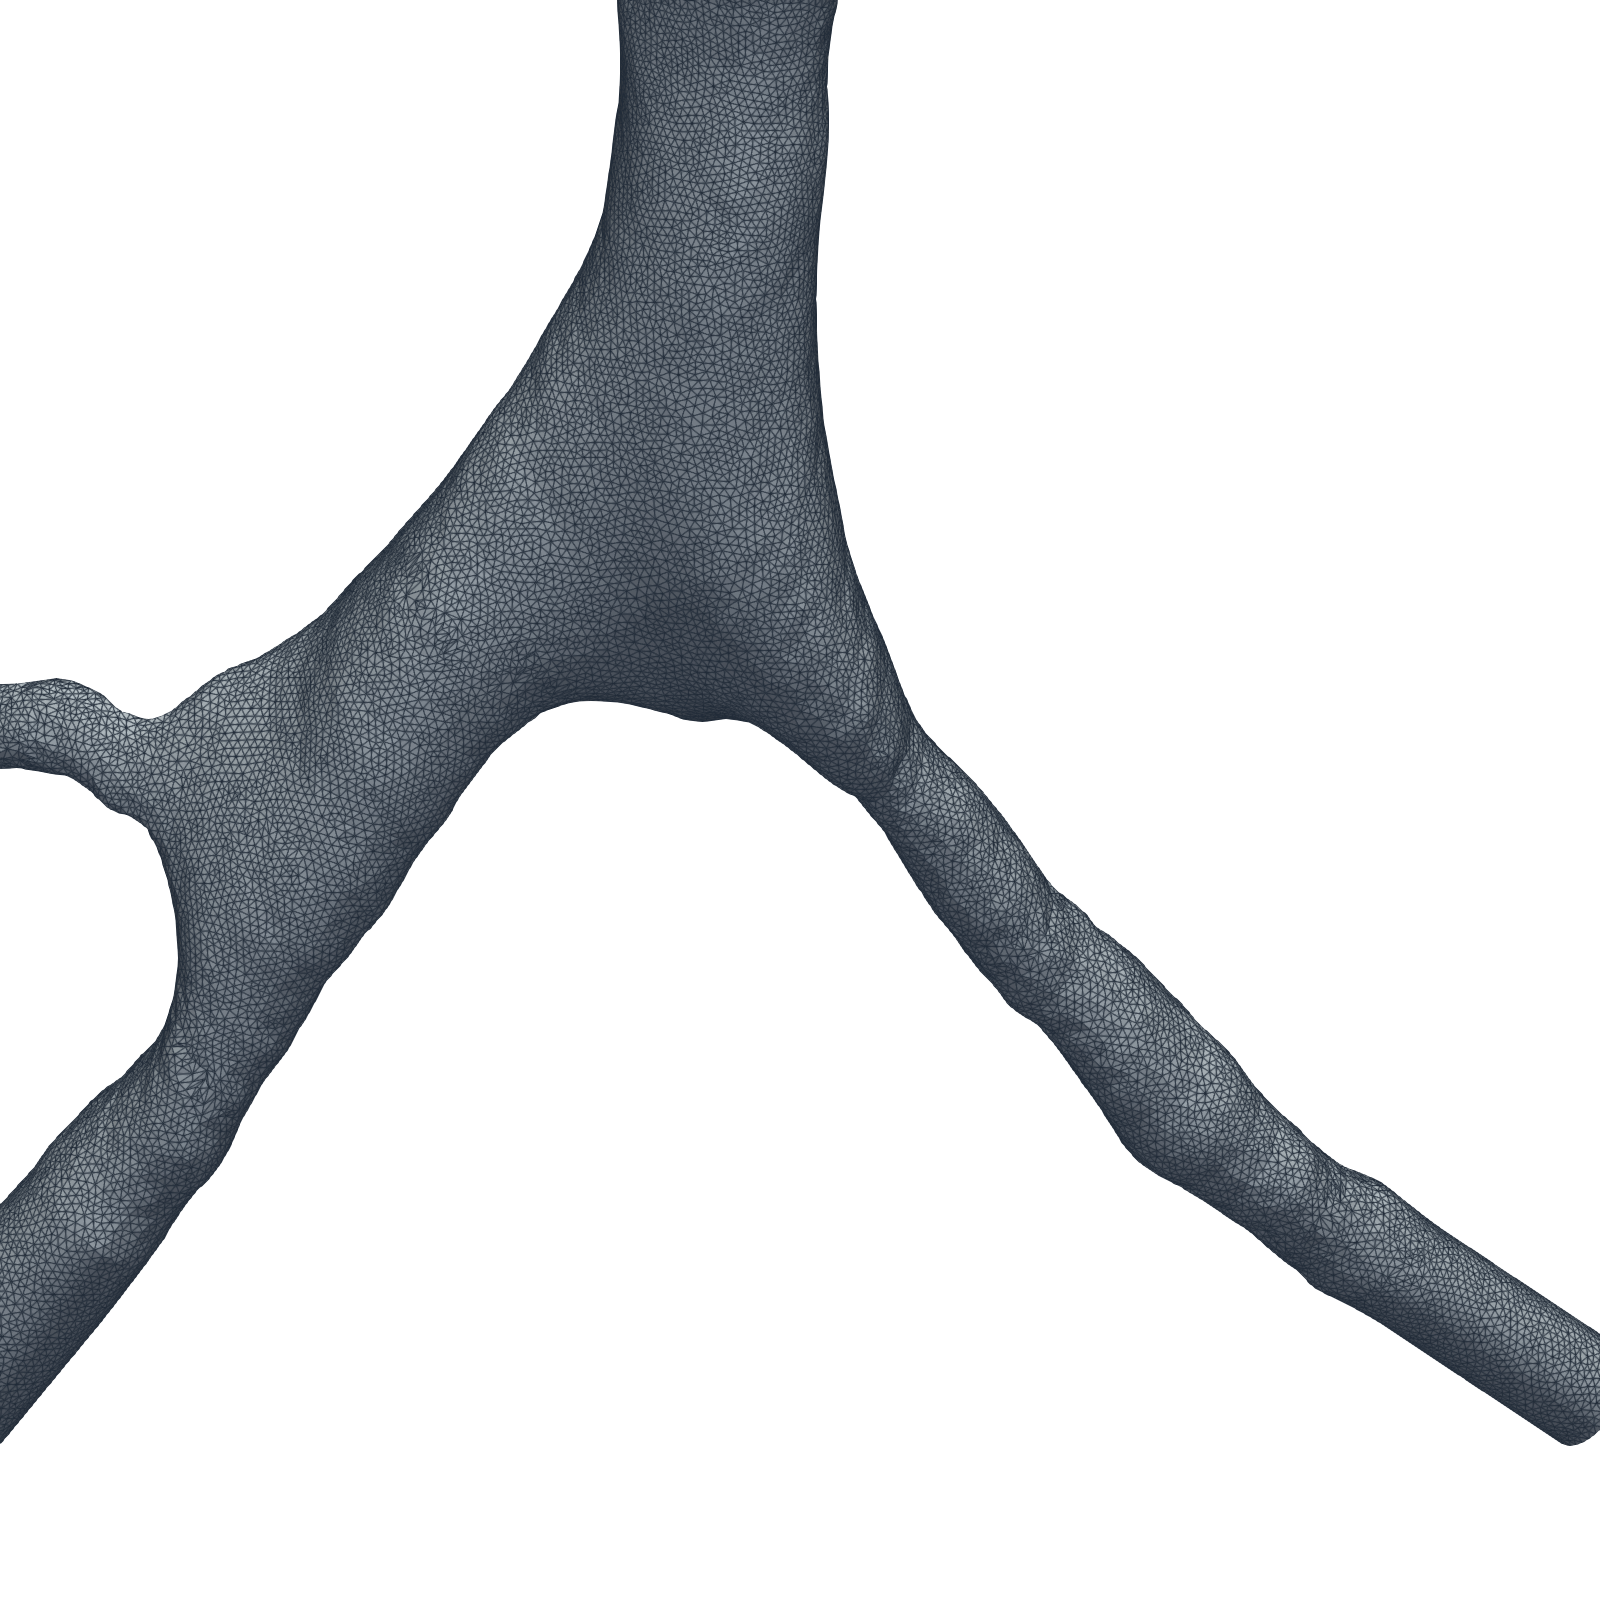
\includegraphics[width=\linewidth]{assignment5_mesh_015_closeup.png}
    \caption{Selected-mesh surface triangulation at the carina.}
  \end{subfigure}
  \caption{Postoperative HXT mesh refinement in matched anatomical frontal
  views. The complete baseline and selected meshes are shown above, with
  identically framed carina close-ups below. Both levels use the same geometry,
  physical surface groups, and HXT algorithm; only target characteristic length
  differs. Surface-edge density illustrates refinement, while quantitative
  volume-mesh sensitivity is assessed separately in
  Section~\ref{sec:mesh_sensitivity}.}
  \label{fig:meshes}
\end{figure}

% -----------------------------------------------------------------------------
\section{Mathematical model}
\label{sec:model}

\subsection{Governing equations}

Air is modelled as an incompressible Newtonian fluid. For steady flow, mass and
momentum conservation are:

\begin{align}
  \nabla \cdot \mathbf{u} &= 0, \\
  \rho (\mathbf{u}\cdot\nabla)\mathbf{u}
    &= -\nabla p + \mu \nabla^2\mathbf{u},
\end{align}

where $\mathbf{u}$ is velocity, $p$ is pressure, $\rho$ is density, and $\mu$
is dynamic viscosity. OpenFOAM uses kinematic pressure and the kinematic
viscosity $\nu=\mu/\rho$. The configured value is
$\nu=\SI{1.5e-5}{\metre\squared\per\second}$.

The current case uses the laminar model and the steady-state
\texttt{simpleFoam} solver. The appropriateness of the laminar assumption should
be assessed using a Reynolds number based on representative velocity $U$ and
diameter $D$:

\begin{equation}
  \mathrm{Re} = \frac{UD}{\nu}.
\end{equation}

[Calculate Reynolds numbers at the inlet and stenosis and discuss whether a
laminar, transitional, or turbulent model is justified.]

\subsection{Boundary conditions}

A prescribed volumetric flow rate is applied at the tracheal inlet:

\begin{equation}
  Q_{\mathrm{in}} = \SI{3.3333e-5}{\metre\cubed\per\second}.
\end{equation}

This corresponds to approximately \SI{2}{\litre\per\minute}, representative
of the stated minute volume for a 10-month-old infant. A no-slip condition is
applied at the airway wall. The three distal outlets use the same zero gauge
pressure with pressure-compatible velocity conditions. No outlet flow fraction
is prescribed; consequently, the flow division is an output of the CFD solution.
For a common downstream pressure, each pathway behaves approximately as

\begin{equation}
  Q_i \sim \frac{\Delta P}{R_i},
\end{equation}

where differences in effective resistance $R_i$ arise from features such as
branch diameter, length, branching angle, curvature, and flow separation.
Table~\ref{tab:bc} summarises the implementation.

\begin{table}[htbp]
  \centering
  \caption{OpenFOAM boundary conditions.}
  \label{tab:bc}
  \begin{tabular}{@{}lll@{}}
    \toprule
    Patch & Velocity $\mathbf{u}$ & Pressure $p$ \\
    \midrule
    \texttt{inlet} & \texttt{flowRateInletVelocity} & \texttt{zeroGradient} \\
    \texttt{outlet\_1--3} & \texttt{pressureInletOutletVelocity} & \texttt{fixedValue 0} \\
    \texttt{wall} & \texttt{noSlip} & \texttt{zeroGradient} \\
    \bottomrule
  \end{tabular}
\end{table}

% -----------------------------------------------------------------------------
\section{Numerical method}
\label{sec:numerics}

The teaching staff approved the use of 3D Slicer and SlicerVMTK for geometry
preparation, Gmsh for meshing, OpenFOAM for CFD, and independent local/remote
compute infrastructure. This changes the software implementation but not the
required physical analyses or validation.

\begin{table}[htbp]
  \centering
  \caption{Software and provenance information. Replace placeholders with the
  immutable versions used for the final simulations.}
  \label{tab:software}
  \begin{tabular}{@{}lll@{}}
    \toprule
    Stage & Software & Version or identifier \\
    \midrule
    Segmentation & 3D Slicer + SlicerVMTK & 5.12.2; extension [insert] \\
    Surface/volume meshing & Gmsh & [insert] \\
    CFD & OpenFOAM Docker image & 2512; image ID [insert] \\
    Post-processing & ParaView & [insert] \\
    Source state & Git & commit [insert] \\
    \bottomrule
  \end{tabular}
\end{table}

\subsection{Steady solver}

The finite-volume discretisation is implemented in OpenFOAM 2512. Pressure is
solved using GAMG and velocity using a symmetric Gauss--Seidel smoothed solver.
The SIMPLE algorithm uses two non-orthogonal correctors. The configured residual
controls are $10^{-5}$ for pressure and $10^{-6}$ for velocity.

The parallel mesh is decomposed using the Scotch method. Simulations are run in
the \texttt{opencfd/openfoam-default:latest} Docker image. The exact image ID
and Git commit are recorded in Table~\ref{tab:software}.

\subsection{Transient solver and breathing waveform}
\label{sec:transient_method}

The initially selected \num{0.15}~mm HXT mesh proved computationally
impractical for the complete postoperative cycle. The final transient analysis
is therefore an explicitly labelled proof of concept on the existing
\num{0.25}~mm HXT mesh (180,163 tetrahedra). The incompressible, Newtonian
equations are solved with \texttt{pimpleFoam}. A symmetric sinusoidal volumetric-flow boundary condition is
prescribed at the tracheal inlet,
\begin{equation}
  Q(t)=Q_{\max}\sin\left(\frac{2\pi t}{T}\right),
\end{equation}
where $T=\SI{2.0}{\second}$ and
$Q_{\max}=\SI{1.0472e-4}{\metre\cubed\per\second}$
(\SI{6.283}{\litre\per\minute}). The positive half-cycle represents inspiration
and the negative half-cycle expiration. Integrating either half-cycle gives a
tidal volume of \SI{66.7}{\milli\litre}, consistent with the assumed
\SI{2}{\litre\per\minute} minute ventilation at 30 breaths per minute.

The inlet uses \texttt{flowRateInletVelocity}. All three outlets have zero fixed
kinematic pressure and \texttt{pressureInletOutletVelocity}, which permits flow
reversal during expiration. The rigid airway wall remains no-slip. Time is
discretised with the second-order backward scheme and bounded first-order upwind
convection. Three PIMPLE outer correctors, two pressure correctors, and two
non-orthogonal correctors are used. An initial time step of
\SI{1e-5}{\second} is adjusted subject to $\mathrm{Co}_{\max}=5$ and a maximum
step of \SI{2e-4}{\second}; fields are written every \SI{0.02}{\second}. A
conservative timing run at $\mathrm{Co}_{\max}=2$ established stable coupling,
but projected runtime remained prohibitive. The final $\mathrm{Co}_{\max}=5$
case completed on eight MPI ranks in \SI{65095}{\second} wall time. This elevated
Courant limit, coarse mesh, and diffusive convection scheme permit workflow and
phase-trend assessment but preclude claims of temporal or spatial independence.
Periodicity also cannot be claimed from the single cycle starting from rest.

At the estimated peak mean velocity of approximately
\SI{20.3}{\metre\per\second} in the matched section, the Mach number is about
0.06, supporting the incompressibility approximation. The corresponding Reynolds
number is approximately 3500, so transitional effects remain a model limitation.
A shorter, more realistic mechanically ventilated inspiratory phase would require
a larger peak flow for the same tidal volume and could approach the commonly used
$\mathrm{Ma}=0.1$ compressibility threshold.

\begin{figure}[htbp]
  \centering
  \resizebox{0.88\textwidth}{!}{% GNUPLOT: LaTeX picture with Postscript
\begingroup
  \makeatletter
  \providecommand\color[2][]{%
    \GenericError{(gnuplot) \space\space\space\@spaces}{%
      Package color not loaded in conjunction with
      terminal option `colourtext'%
    }{See the gnuplot documentation for explanation.%
    }{Either use 'blacktext' in gnuplot or load the package
      color.sty in LaTeX.}%
    \renewcommand\color[2][]{}%
  }%
  \providecommand\includegraphics[2][]{%
    \GenericError{(gnuplot) \space\space\space\@spaces}{%
      Package graphicx or graphics not loaded%
    }{See the gnuplot documentation for explanation.%
    }{The gnuplot epslatex terminal needs graphicx.sty or graphics.sty.}%
    \renewcommand\includegraphics[2][]{}%
  }%
  \providecommand\rotatebox[2]{#2}%
  \@ifundefined{ifGPcolor}{%
    \newif\ifGPcolor
    \GPcolortrue
  }{}%
  \@ifundefined{ifGPblacktext}{%
    \newif\ifGPblacktext
    \GPblacktexttrue
  }{}%
  % define a \g@addto@macro without @ in the name:
  \let\gplgaddtomacro\g@addto@macro
  % define empty templates for all commands taking text:
  \gdef\gplbacktext{}%
  \gdef\gplfronttext{}%
  \makeatother
  \ifGPblacktext
    % no textcolor at all
    \def\colorrgb#1{}%
    \def\colorgray#1{}%
  \else
    % gray or color?
    \ifGPcolor
      \def\colorrgb#1{\color[rgb]{#1}}%
      \def\colorgray#1{\color[gray]{#1}}%
      \expandafter\def\csname LTw\endcsname{\color{white}}%
      \expandafter\def\csname LTb\endcsname{\color{black}}%
      \expandafter\def\csname LTa\endcsname{\color{black}}%
      \expandafter\def\csname LT0\endcsname{\color[rgb]{1,0,0}}%
      \expandafter\def\csname LT1\endcsname{\color[rgb]{0,1,0}}%
      \expandafter\def\csname LT2\endcsname{\color[rgb]{0,0,1}}%
      \expandafter\def\csname LT3\endcsname{\color[rgb]{1,0,1}}%
      \expandafter\def\csname LT4\endcsname{\color[rgb]{0,1,1}}%
      \expandafter\def\csname LT5\endcsname{\color[rgb]{1,1,0}}%
      \expandafter\def\csname LT6\endcsname{\color[rgb]{0,0,0}}%
      \expandafter\def\csname LT7\endcsname{\color[rgb]{1,0.3,0}}%
      \expandafter\def\csname LT8\endcsname{\color[rgb]{0.5,0.5,0.5}}%
    \else
      % gray
      \def\colorrgb#1{\color{black}}%
      \def\colorgray#1{\color[gray]{#1}}%
      \expandafter\def\csname LTw\endcsname{\color{white}}%
      \expandafter\def\csname LTb\endcsname{\color{black}}%
      \expandafter\def\csname LTa\endcsname{\color{black}}%
      \expandafter\def\csname LT0\endcsname{\color{black}}%
      \expandafter\def\csname LT1\endcsname{\color{black}}%
      \expandafter\def\csname LT2\endcsname{\color{black}}%
      \expandafter\def\csname LT3\endcsname{\color{black}}%
      \expandafter\def\csname LT4\endcsname{\color{black}}%
      \expandafter\def\csname LT5\endcsname{\color{black}}%
      \expandafter\def\csname LT6\endcsname{\color{black}}%
      \expandafter\def\csname LT7\endcsname{\color{black}}%
      \expandafter\def\csname LT8\endcsname{\color{black}}%
    \fi
  \fi
    \setlength{\unitlength}{0.0500bp}%
    \ifx\gptboxheight\undefined%
      \newlength{\gptboxheight}%
      \newlength{\gptboxwidth}%
      \newsavebox{\gptboxtext}%
    \fi%
    \setlength{\fboxrule}{0.5pt}%
    \setlength{\fboxsep}{1pt}%
    \definecolor{tbcol}{rgb}{1,1,1}%
\begin{picture}(8500.00,4520.00)%
    \gplgaddtomacro\gplbacktext{%
      \csname LTb\endcsname%%
      \put(487,562){\makebox(0,0)[r]{\strut{}$-8$}}%
      \csname LTb\endcsname%%
      \put(487,989){\makebox(0,0)[r]{\strut{}$-6$}}%
      \csname LTb\endcsname%%
      \put(487,1415){\makebox(0,0)[r]{\strut{}$-4$}}%
      \csname LTb\endcsname%%
      \put(487,1841){\makebox(0,0)[r]{\strut{}$-2$}}%
      \csname LTb\endcsname%%
      \put(487,2267){\makebox(0,0)[r]{\strut{}$0$}}%
      \csname LTb\endcsname%%
      \put(487,2693){\makebox(0,0)[r]{\strut{}$2$}}%
      \csname LTb\endcsname%%
      \put(487,3119){\makebox(0,0)[r]{\strut{}$4$}}%
      \csname LTb\endcsname%%
      \put(487,3546){\makebox(0,0)[r]{\strut{}$6$}}%
      \csname LTb\endcsname%%
      \put(487,3972){\makebox(0,0)[r]{\strut{}$8$}}%
      \csname LTb\endcsname%%
      \put(576,386){\makebox(0,0){\strut{}$0$}}%
      \csname LTb\endcsname%%
      \put(2485,386){\makebox(0,0){\strut{}$0.5$}}%
      \csname LTb\endcsname%%
      \put(4394,386){\makebox(0,0){\strut{}$1$}}%
      \csname LTb\endcsname%%
      \put(6303,386){\makebox(0,0){\strut{}$1.5$}}%
      \csname LTb\endcsname%%
      \put(8212,386){\makebox(0,0){\strut{}$2$}}%
    }%
    \gplgaddtomacro\gplfronttext{%
      \csname LTb\endcsname%%
      \put(154,2267){\rotatebox{-270.00}{\makebox(0,0){\strut{}Inlet flow rate (L/min)}}}%
      \csname LTb\endcsname%%
      \put(4394,123){\makebox(0,0){\strut{}Time (s)}}%
      \csname LTb\endcsname%%
      \put(4394,4236){\makebox(0,0){\strut{}Sinusoidal breathing waveform}}%
    }%
    \gplbacktext
    \put(0,0){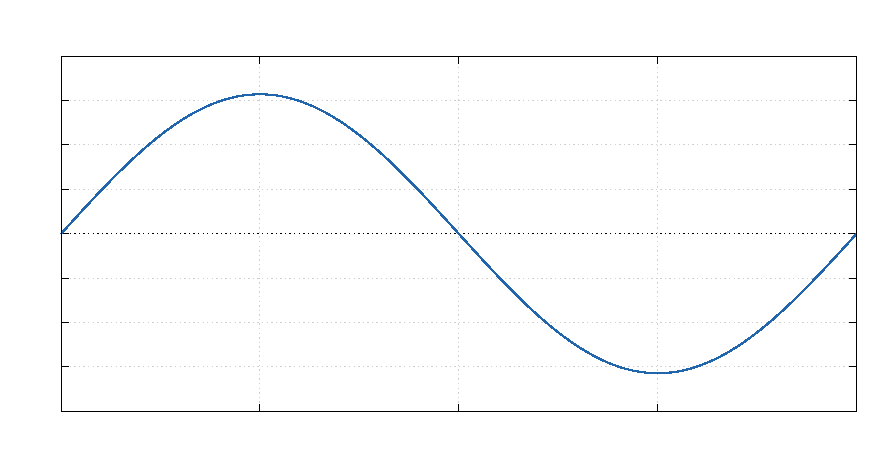
\includegraphics[width={425.00bp},height={226.00bp}]{figures/assignment6_breathing_waveform}}%
    \gplfronttext
  \end{picture}%
\endgroup
}
  \caption{Prescribed sinusoidal inlet flow for the postoperative transient
  simulation. Positive and negative flow denote inspiration and expiration,
  respectively.}
  \label{fig:transient_waveform}
\end{figure}

\begin{table}[htbp]
  \centering
  \caption{Transient postoperative simulation settings.}
  \label{tab:transient_settings}
  \begin{tabular}{@{}ll@{}}
    \toprule
    Parameter & Value \\
    \midrule
    Solver & \texttt{pimpleFoam} \\
    Breathing-cycle duration & \SI{2.0}{\second} \\
    Mesh & HXT, \SI{0.25}{\milli\metre}, 180,163 tetrahedra \\
    Initial / maximum time step & \SI{1e-5}{\second} / \SI{2e-4}{\second} \\
    Maximum Courant number & 5.0 \\
    Field write interval & \SI{0.02}{\second} \\
    Simulated cycles & One, starting from rest \\
    PIMPLE correctors & Up to 3 outer, 2 pressure, 2 non-orthogonal \\
    Outer stopping targets & $2\times10^{-3}$ ($U$), $10^{-2}$ ($p$) \\
    Linear-equation tolerance & $10^{-8}$ ($U$ and $p$) \\
    Parallel decomposition & Scotch, 8 MPI ranks \\
    \bottomrule
  \end{tabular}
\end{table}

% -----------------------------------------------------------------------------
\section{Verification}
\label{sec:verification}

\subsection{Mesh quality}

Table~\ref{tab:mesh_quality} summarises the principal \texttt{checkMesh}
metrics for the four postoperative HXT meshes. All meshes contained one
connected fluid region. A face was counted as severely non-orthogonal when its
non-orthogonality exceeded $70^\circ$.

\begin{table}[htbp]
  \centering
  \caption{Postoperative HXT mesh-quality metrics reported by
  \texttt{checkMesh}. The minimum cell volumes are given after conversion of
  the geometry from millimetres to metres.}
  \label{tab:mesh_quality}
  \resizebox{\textwidth}{!}{%
  \begin{tabular}{@{}lrrrrrr@{}}
    \toprule
    Target size & Max. aspect ratio & Max. non-orthogonality & Severe faces & Max. skewness & Min. volume (\si{\metre\cubed}) & Regions \\
    \midrule
    \SI{0.25}{\milli\metre} & 114.14 & $88.63^\circ$ & 2  & 1.457 & $7.90\times10^{-15}$ & 1 \\
    \SI{0.20}{\milli\metre} & 11.73  & $80.29^\circ$ & 2  & 1.268 & $3.64\times10^{-14}$ & 1 \\
    \SI{0.15}{\milli\metre} & 12.63  & $69.82^\circ$ & 0  & 1.196 & $5.12\times10^{-14}$ & 1 \\
    \SI{0.12}{\milli\metre} & 88.00  & $82.34^\circ$ & 19 & 1.396 & $8.71\times10^{-16}$ & 1 \\
    \bottomrule
  \end{tabular}%
  }
\end{table}

The \SI{0.15}{\milli\metre} mesh had the strongest overall quality: its maximum
non-orthogonality remained below $70^\circ$, it contained no severely
non-orthogonal faces, and it had the lowest maximum skewness of the series. Its
maximum aspect ratio of 12.63 was also substantially lower than those of the
\SI{0.25}{\milli\metre} and \SI{0.12}{\milli\metre} meshes. Refining the target
size did not improve every quality measure monotonically. In particular, the
\SI{0.12}{\milli\metre} mesh introduced 19 severely non-orthogonal faces, a
maximum aspect ratio of 88.00, and the smallest cell volume in the series. This
local deterioration is consistent with its poorer solver convergence and shows
why cell count alone is not a sufficient mesh-selection criterion. Nevertheless,
all four meshes remained single connected domains and their maximum skewness was
below the OpenFOAM internal-cell warning limit of 4. The quality results therefore
support selection of the \SI{0.15}{\milli\metre} mesh for the final analysis.

\subsection{Convergence and mass conservation}

The SIMPLE solution met residual control after 589 iterations. Final initial
residuals were $9.93\times10^{-7}$, $7.57\times10^{-7}$, and
$6.48\times10^{-7}$ for $U_x$, $U_y$, and $U_z$, respectively, and
$4.92\times10^{-6}$ for pressure. These are below the configured criteria of
$10^{-6}$ for velocity and $10^{-5}$ for pressure. Final outlet-flow integration
is still used to verify that

\begin{equation}
  Q_{\mathrm{in}} + \sum_{i=1}^{3} Q_{\mathrm{out},i} \approx 0,
\end{equation}

using a consistent outward-normal sign convention. Report the relative mass
imbalance.

\begin{figure}[htbp]
  \centering
  \resizebox{0.95\textwidth}{!}{% GNUPLOT: LaTeX picture with Postscript
\begingroup
  \makeatletter
  \providecommand\color[2][]{%
    \GenericError{(gnuplot) \space\space\space\@spaces}{%
      Package color not loaded in conjunction with
      terminal option `colourtext'%
    }{See the gnuplot documentation for explanation.%
    }{Either use 'blacktext' in gnuplot or load the package
      color.sty in LaTeX.}%
    \renewcommand\color[2][]{}%
  }%
  \providecommand\includegraphics[2][]{%
    \GenericError{(gnuplot) \space\space\space\@spaces}{%
      Package graphicx or graphics not loaded%
    }{See the gnuplot documentation for explanation.%
    }{The gnuplot epslatex terminal needs graphicx.sty or graphics.sty.}%
    \renewcommand\includegraphics[2][]{}%
  }%
  \providecommand\rotatebox[2]{#2}%
  \@ifundefined{ifGPcolor}{%
    \newif\ifGPcolor
    \GPcolortrue
  }{}%
  \@ifundefined{ifGPblacktext}{%
    \newif\ifGPblacktext
    \GPblacktexttrue
  }{}%
  % define a \g@addto@macro without @ in the name:
  \let\gplgaddtomacro\g@addto@macro
  % define empty templates for all commands taking text:
  \gdef\gplbacktext{}%
  \gdef\gplfronttext{}%
  \makeatother
  \ifGPblacktext
    % no textcolor at all
    \def\colorrgb#1{}%
    \def\colorgray#1{}%
  \else
    % gray or color?
    \ifGPcolor
      \def\colorrgb#1{\color[rgb]{#1}}%
      \def\colorgray#1{\color[gray]{#1}}%
      \expandafter\def\csname LTw\endcsname{\color{white}}%
      \expandafter\def\csname LTb\endcsname{\color{black}}%
      \expandafter\def\csname LTa\endcsname{\color{black}}%
      \expandafter\def\csname LT0\endcsname{\color[rgb]{1,0,0}}%
      \expandafter\def\csname LT1\endcsname{\color[rgb]{0,1,0}}%
      \expandafter\def\csname LT2\endcsname{\color[rgb]{0,0,1}}%
      \expandafter\def\csname LT3\endcsname{\color[rgb]{1,0,1}}%
      \expandafter\def\csname LT4\endcsname{\color[rgb]{0,1,1}}%
      \expandafter\def\csname LT5\endcsname{\color[rgb]{1,1,0}}%
      \expandafter\def\csname LT6\endcsname{\color[rgb]{0,0,0}}%
      \expandafter\def\csname LT7\endcsname{\color[rgb]{1,0.3,0}}%
      \expandafter\def\csname LT8\endcsname{\color[rgb]{0.5,0.5,0.5}}%
    \else
      % gray
      \def\colorrgb#1{\color{black}}%
      \def\colorgray#1{\color[gray]{#1}}%
      \expandafter\def\csname LTw\endcsname{\color{white}}%
      \expandafter\def\csname LTb\endcsname{\color{black}}%
      \expandafter\def\csname LTa\endcsname{\color{black}}%
      \expandafter\def\csname LT0\endcsname{\color{black}}%
      \expandafter\def\csname LT1\endcsname{\color{black}}%
      \expandafter\def\csname LT2\endcsname{\color{black}}%
      \expandafter\def\csname LT3\endcsname{\color{black}}%
      \expandafter\def\csname LT4\endcsname{\color{black}}%
      \expandafter\def\csname LT5\endcsname{\color{black}}%
      \expandafter\def\csname LT6\endcsname{\color{black}}%
      \expandafter\def\csname LT7\endcsname{\color{black}}%
      \expandafter\def\csname LT8\endcsname{\color{black}}%
    \fi
  \fi
    \setlength{\unitlength}{0.0500bp}%
    \ifx\gptboxheight\undefined%
      \newlength{\gptboxheight}%
      \newlength{\gptboxwidth}%
      \newsavebox{\gptboxtext}%
    \fi%
    \setlength{\fboxrule}{0.5pt}%
    \setlength{\fboxsep}{1pt}%
    \definecolor{tbcol}{rgb}{1,1,1}%
\begin{picture}(8500.00,5100.00)%
    \gplgaddtomacro\gplbacktext{%
      \csname LTb\endcsname%%
      \put(665,562){\makebox(0,0)[r]{\strut{}$10^{-7}$}}%
      \csname LTb\endcsname%%
      \put(665,1082){\makebox(0,0)[r]{\strut{}$10^{-6}$}}%
      \csname LTb\endcsname%%
      \put(665,1602){\makebox(0,0)[r]{\strut{}$10^{-5}$}}%
      \csname LTb\endcsname%%
      \put(665,2121){\makebox(0,0)[r]{\strut{}$10^{-4}$}}%
      \csname LTb\endcsname%%
      \put(665,2641){\makebox(0,0)[r]{\strut{}$10^{-3}$}}%
      \csname LTb\endcsname%%
      \put(665,3161){\makebox(0,0)[r]{\strut{}$10^{-2}$}}%
      \csname LTb\endcsname%%
      \put(665,3680){\makebox(0,0)[r]{\strut{}$10^{-1}$}}%
      \csname LTb\endcsname%%
      \put(665,4200){\makebox(0,0)[r]{\strut{}$10^{0}$}}%
      \csname LTb\endcsname%%
      \put(1579,386){\makebox(0,0){\strut{}$200$}}%
      \csname LTb\endcsname%%
      \put(2408,386){\makebox(0,0){\strut{}$400$}}%
      \csname LTb\endcsname%%
      \put(3237,386){\makebox(0,0){\strut{}$600$}}%
      \csname LTb\endcsname%%
      \put(4067,386){\makebox(0,0){\strut{}$800$}}%
      \csname LTb\endcsname%%
      \put(4896,386){\makebox(0,0){\strut{}$1000$}}%
      \csname LTb\endcsname%%
      \put(5725,386){\makebox(0,0){\strut{}$1200$}}%
      \csname LTb\endcsname%%
      \put(6554,386){\makebox(0,0){\strut{}$1400$}}%
      \csname LTb\endcsname%%
      \put(7383,386){\makebox(0,0){\strut{}$1600$}}%
      \csname LTb\endcsname%%
      \put(8212,386){\makebox(0,0){\strut{}$1800$}}%
    }%
    \gplgaddtomacro\gplfronttext{%
      \csname LTb\endcsname%%
      \put(3087,4921){\makebox(0,0)[r]{\strut{}$U_x$}}%
      \csname LTb\endcsname%%
      \put(3087,4745){\makebox(0,0)[r]{\strut{}$U_y$}}%
      \csname LTb\endcsname%%
      \put(4671,4921){\makebox(0,0)[r]{\strut{}$U_z$}}%
      \csname LTb\endcsname%%
      \put(4671,4745){\makebox(0,0)[r]{\strut{}$p$}}%
      \csname LTb\endcsname%%
      \put(6254,4921){\makebox(0,0)[r]{\strut{}$U$ criterion}}%
      \csname LTb\endcsname%%
      \put(6254,4745){\makebox(0,0)[r]{\strut{}$p$ criterion}}%
      \csname LTb\endcsname%%
      \put(154,2381){\rotatebox{-270.00}{\makebox(0,0){\strut{}Initial residual}}}%
      \csname LTb\endcsname%%
      \put(4483,123){\makebox(0,0){\strut{}SIMPLE iteration}}%
      \csname LTb\endcsname%%
      \put(4483,4464){\makebox(0,0){\strut{}Postoperative steady-solver convergence}}%
    }%
    \gplbacktext
    \put(0,0){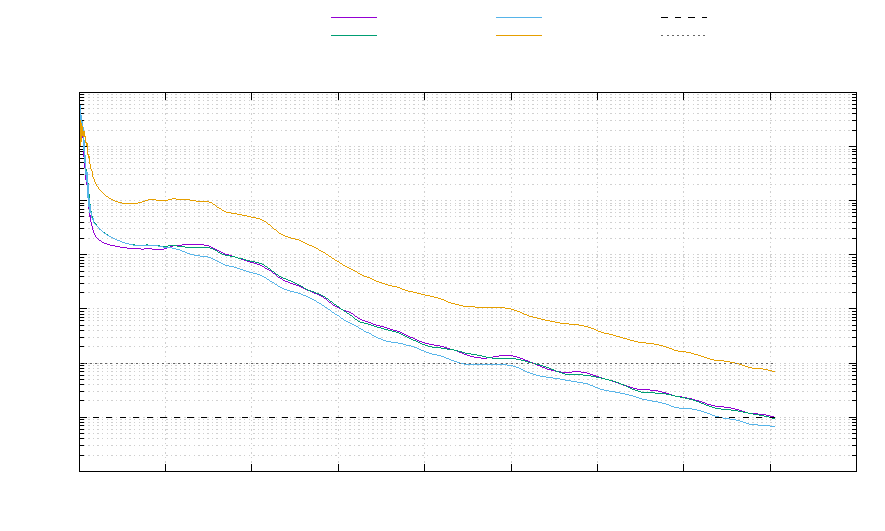
\includegraphics[width={425.00bp},height={255.00bp}]{figures/assignment4_residuals}}%
    \gplfronttext
  \end{picture}%
\endgroup
}
  \caption{Initial residual evolution for the postoperative steady simulation.
  Dashed and dotted lines indicate the configured velocity and pressure
  convergence criteria. The SIMPLE algorithm stopped at iteration 589 after all
  criteria were satisfied.}
  \label{fig:steady_residuals}
\end{figure}

\subsection{Effect of additional steady iterations}

Assignment 4 requests an assessment of whether 1000 additional iterations alter
an axial-velocity parameter. A fixed centerline-normal section before the
bifurcation is used, and its area-averaged axial velocity is recorded before and
after continuation without reinitialising the solution.

\begin{table}[htbp]
  \centering
  \caption{Sensitivity of the selected axial-velocity monitor to 1000 additional
  steady iterations.}
  \label{tab:additional_iterations}
  \begin{tabular}{@{}lrrr@{}}
    \toprule
    Parameter & Iteration 2000 & Iteration 3000 & Relative change (\%) \\
    \midrule
    Area-averaged axial velocity & [insert] & [insert] & [insert] \\
    \bottomrule
  \end{tabular}
\end{table}

\subsection{Mesh-independence assessment}
\label{sec:mesh_sensitivity}

At least three postoperative mesh levels are preferred so that a trend can be
assessed rather than only a pairwise difference. Each parameter of interest is
plotted against the number of volume elements. For mesh $i$ and the densest mesh
$d$, the Assignment 5 percentage difference is defined as

\begin{equation}
  \delta_{\phi,i} =
  \frac{|\phi_i-\phi_d|}{|\phi_d|}\times 100\%.
  \label{eq:mesh_difference}
\end{equation}

\begin{table}[htbp]
  \centering
  \caption{Mesh-independence comparison.}
  \label{tab:mesh_independence}
  \begin{tabular}{@{}lrrrr@{}}
    \toprule
    Quantity & 0.25 mm & 0.20 mm & 0.15 mm & 0.12 mm \\
    \midrule
    Resistance (Pa/(L/min)) & 15.153 & 16.361 & 17.544 & 17.906 \\
    Peak velocity (m/s) & 9.447 & 9.573 & 9.670 & 9.822 \\
    Right-lung fraction (\%) & 73.664 & 73.619 & 73.686 & 73.397 \\
    Right-superior share (\%) & 15.231 & 15.597 & 16.017 & 16.250 \\
    Solver iterations & 596 & 770 & 1611 & 2000$^*$ \\
    \bottomrule
  \end{tabular}
  \\[2pt]\footnotesize{$^*$Iteration limit reached without satisfying residual control.}
\end{table}

\begin{figure}[htbp]
  \centering
  \resizebox{0.98\textwidth}{!}{% GNUPLOT: LaTeX picture with Postscript
\begingroup
  \makeatletter
  \providecommand\color[2][]{%
    \GenericError{(gnuplot) \space\space\space\@spaces}{%
      Package color not loaded in conjunction with
      terminal option `colourtext'%
    }{See the gnuplot documentation for explanation.%
    }{Either use 'blacktext' in gnuplot or load the package
      color.sty in LaTeX.}%
    \renewcommand\color[2][]{}%
  }%
  \providecommand\includegraphics[2][]{%
    \GenericError{(gnuplot) \space\space\space\@spaces}{%
      Package graphicx or graphics not loaded%
    }{See the gnuplot documentation for explanation.%
    }{The gnuplot epslatex terminal needs graphicx.sty or graphics.sty.}%
    \renewcommand\includegraphics[2][]{}%
  }%
  \providecommand\rotatebox[2]{#2}%
  \@ifundefined{ifGPcolor}{%
    \newif\ifGPcolor
    \GPcolortrue
  }{}%
  \@ifundefined{ifGPblacktext}{%
    \newif\ifGPblacktext
    \GPblacktexttrue
  }{}%
  % define a \g@addto@macro without @ in the name:
  \let\gplgaddtomacro\g@addto@macro
  % define empty templates for all commands taking text:
  \gdef\gplbacktext{}%
  \gdef\gplfronttext{}%
  \makeatother
  \ifGPblacktext
    % no textcolor at all
    \def\colorrgb#1{}%
    \def\colorgray#1{}%
  \else
    % gray or color?
    \ifGPcolor
      \def\colorrgb#1{\color[rgb]{#1}}%
      \def\colorgray#1{\color[gray]{#1}}%
      \expandafter\def\csname LTw\endcsname{\color{white}}%
      \expandafter\def\csname LTb\endcsname{\color{black}}%
      \expandafter\def\csname LTa\endcsname{\color{black}}%
      \expandafter\def\csname LT0\endcsname{\color[rgb]{1,0,0}}%
      \expandafter\def\csname LT1\endcsname{\color[rgb]{0,1,0}}%
      \expandafter\def\csname LT2\endcsname{\color[rgb]{0,0,1}}%
      \expandafter\def\csname LT3\endcsname{\color[rgb]{1,0,1}}%
      \expandafter\def\csname LT4\endcsname{\color[rgb]{0,1,1}}%
      \expandafter\def\csname LT5\endcsname{\color[rgb]{1,1,0}}%
      \expandafter\def\csname LT6\endcsname{\color[rgb]{0,0,0}}%
      \expandafter\def\csname LT7\endcsname{\color[rgb]{1,0.3,0}}%
      \expandafter\def\csname LT8\endcsname{\color[rgb]{0.5,0.5,0.5}}%
    \else
      % gray
      \def\colorrgb#1{\color{black}}%
      \def\colorgray#1{\color[gray]{#1}}%
      \expandafter\def\csname LTw\endcsname{\color{white}}%
      \expandafter\def\csname LTb\endcsname{\color{black}}%
      \expandafter\def\csname LTa\endcsname{\color{black}}%
      \expandafter\def\csname LT0\endcsname{\color{black}}%
      \expandafter\def\csname LT1\endcsname{\color{black}}%
      \expandafter\def\csname LT2\endcsname{\color{black}}%
      \expandafter\def\csname LT3\endcsname{\color{black}}%
      \expandafter\def\csname LT4\endcsname{\color{black}}%
      \expandafter\def\csname LT5\endcsname{\color{black}}%
      \expandafter\def\csname LT6\endcsname{\color{black}}%
      \expandafter\def\csname LT7\endcsname{\color{black}}%
      \expandafter\def\csname LT8\endcsname{\color{black}}%
    \fi
  \fi
    \setlength{\unitlength}{0.0500bp}%
    \ifx\gptboxheight\undefined%
      \newlength{\gptboxheight}%
      \newlength{\gptboxwidth}%
      \newsavebox{\gptboxtext}%
    \fi%
    \setlength{\fboxrule}{0.5pt}%
    \setlength{\fboxsep}{1pt}%
    \definecolor{tbcol}{rgb}{1,1,1}%
\begin{picture}(9060.00,7360.00)%
    \gplgaddtomacro\gplbacktext{%
      \csname LTb\endcsname%%
      \put(598,4176){\makebox(0,0)[r]{\strut{}$15$}}%
      \csname LTb\endcsname%%
      \put(598,4624){\makebox(0,0)[r]{\strut{}$15.5$}}%
      \csname LTb\endcsname%%
      \put(598,5072){\makebox(0,0)[r]{\strut{}$16$}}%
      \csname LTb\endcsname%%
      \put(598,5520){\makebox(0,0)[r]{\strut{}$16.5$}}%
      \csname LTb\endcsname%%
      \put(598,5968){\makebox(0,0)[r]{\strut{}$17$}}%
      \csname LTb\endcsname%%
      \put(598,6416){\makebox(0,0)[r]{\strut{}$17.5$}}%
      \csname LTb\endcsname%%
      \put(598,6864){\makebox(0,0)[r]{\strut{}$18$}}%
      \csname LTb\endcsname%%
      \put(679,4018){\makebox(0,0){\strut{}0.0$\times10^{0}$}}%
      \csname LTb\endcsname%%
      \put(1129,4018){\makebox(0,0){\strut{}2.0$\times10^{5}$}}%
      \csname LTb\endcsname%%
      \put(1579,4018){\makebox(0,0){\strut{}4.0$\times10^{5}$}}%
      \csname LTb\endcsname%%
      \put(2029,4018){\makebox(0,0){\strut{}6.0$\times10^{5}$}}%
      \csname LTb\endcsname%%
      \put(2479,4018){\makebox(0,0){\strut{}8.0$\times10^{5}$}}%
      \csname LTb\endcsname%%
      \put(2929,4018){\makebox(0,0){\strut{}1.0$\times10^{6}$}}%
      \csname LTb\endcsname%%
      \put(3379,4018){\makebox(0,0){\strut{}1.2$\times10^{6}$}}%
      \csname LTb\endcsname%%
      \put(3829,4018){\makebox(0,0){\strut{}1.4$\times10^{6}$}}%
      \csname LTb\endcsname%%
      \put(4279,4018){\makebox(0,0){\strut{}1.6$\times10^{6}$}}%
    }%
    \gplgaddtomacro\gplfronttext{%
      \csname LTb\endcsname%%
      \put(139,5520){\rotatebox{-270.00}{\makebox(0,0){\strut{}Resistance (Pa/(L/min))}}}%
      \csname LTb\endcsname%%
      \put(2479,3780){\makebox(0,0){\strut{}Number of volume cells}}%
      \csname LTb\endcsname%%
      \put(2479,7102){\makebox(0,0){\strut{}Resistance (Pa/(L/min))}}%
    }%
    \gplgaddtomacro\gplbacktext{%
      \csname LTb\endcsname%%
      \put(5199,4176){\makebox(0,0)[r]{\strut{}$73.35$}}%
      \csname LTb\endcsname%%
      \put(5199,4560){\makebox(0,0)[r]{\strut{}$73.4$}}%
      \csname LTb\endcsname%%
      \put(5199,4944){\makebox(0,0)[r]{\strut{}$73.45$}}%
      \csname LTb\endcsname%%
      \put(5199,5328){\makebox(0,0)[r]{\strut{}$73.5$}}%
      \csname LTb\endcsname%%
      \put(5199,5712){\makebox(0,0)[r]{\strut{}$73.55$}}%
      \csname LTb\endcsname%%
      \put(5199,6096){\makebox(0,0)[r]{\strut{}$73.6$}}%
      \csname LTb\endcsname%%
      \put(5199,6480){\makebox(0,0)[r]{\strut{}$73.65$}}%
      \csname LTb\endcsname%%
      \put(5199,6864){\makebox(0,0)[r]{\strut{}$73.7$}}%
      \csname LTb\endcsname%%
      \put(5279,4018){\makebox(0,0){\strut{}0.0$\times10^{0}$}}%
      \csname LTb\endcsname%%
      \put(5719,4018){\makebox(0,0){\strut{}2.0$\times10^{5}$}}%
      \csname LTb\endcsname%%
      \put(6159,4018){\makebox(0,0){\strut{}4.0$\times10^{5}$}}%
      \csname LTb\endcsname%%
      \put(6599,4018){\makebox(0,0){\strut{}6.0$\times10^{5}$}}%
      \csname LTb\endcsname%%
      \put(7039,4018){\makebox(0,0){\strut{}8.0$\times10^{5}$}}%
      \csname LTb\endcsname%%
      \put(7479,4018){\makebox(0,0){\strut{}1.0$\times10^{6}$}}%
      \csname LTb\endcsname%%
      \put(7919,4018){\makebox(0,0){\strut{}1.2$\times10^{6}$}}%
      \csname LTb\endcsname%%
      \put(8359,4018){\makebox(0,0){\strut{}1.4$\times10^{6}$}}%
      \csname LTb\endcsname%%
      \put(8799,4018){\makebox(0,0){\strut{}1.6$\times10^{6}$}}%
    }%
    \gplgaddtomacro\gplfronttext{%
      \csname LTb\endcsname%%
      \put(4659,5520){\rotatebox{-270.00}{\makebox(0,0){\strut{}Right-lung flow fraction (\%)}}}%
      \csname LTb\endcsname%%
      \put(7039,3780){\makebox(0,0){\strut{}Number of volume cells}}%
      \csname LTb\endcsname%%
      \put(7039,7102){\makebox(0,0){\strut{}Right-lung flow fraction (\%)}}%
    }%
    \gplgaddtomacro\gplbacktext{%
      \csname LTb\endcsname%%
      \put(598,506){\makebox(0,0)[r]{\strut{}$15.2$}}%
      \csname LTb\endcsname%%
      \put(598,954){\makebox(0,0)[r]{\strut{}$15.4$}}%
      \csname LTb\endcsname%%
      \put(598,1402){\makebox(0,0)[r]{\strut{}$15.6$}}%
      \csname LTb\endcsname%%
      \put(598,1850){\makebox(0,0)[r]{\strut{}$15.8$}}%
      \csname LTb\endcsname%%
      \put(598,2298){\makebox(0,0)[r]{\strut{}$16$}}%
      \csname LTb\endcsname%%
      \put(598,2746){\makebox(0,0)[r]{\strut{}$16.2$}}%
      \csname LTb\endcsname%%
      \put(598,3194){\makebox(0,0)[r]{\strut{}$16.4$}}%
      \csname LTb\endcsname%%
      \put(679,348){\makebox(0,0){\strut{}0.0$\times10^{0}$}}%
      \csname LTb\endcsname%%
      \put(1129,348){\makebox(0,0){\strut{}2.0$\times10^{5}$}}%
      \csname LTb\endcsname%%
      \put(1579,348){\makebox(0,0){\strut{}4.0$\times10^{5}$}}%
      \csname LTb\endcsname%%
      \put(2029,348){\makebox(0,0){\strut{}6.0$\times10^{5}$}}%
      \csname LTb\endcsname%%
      \put(2479,348){\makebox(0,0){\strut{}8.0$\times10^{5}$}}%
      \csname LTb\endcsname%%
      \put(2929,348){\makebox(0,0){\strut{}1.0$\times10^{6}$}}%
      \csname LTb\endcsname%%
      \put(3379,348){\makebox(0,0){\strut{}1.2$\times10^{6}$}}%
      \csname LTb\endcsname%%
      \put(3829,348){\makebox(0,0){\strut{}1.4$\times10^{6}$}}%
      \csname LTb\endcsname%%
      \put(4279,348){\makebox(0,0){\strut{}1.6$\times10^{6}$}}%
    }%
    \gplgaddtomacro\gplfronttext{%
      \csname LTb\endcsname%%
      \put(139,1850){\rotatebox{-270.00}{\makebox(0,0){\strut{}Right-superior share of right flow (\%)}}}%
      \csname LTb\endcsname%%
      \put(2479,110){\makebox(0,0){\strut{}Number of volume cells}}%
      \csname LTb\endcsname%%
      \put(2479,3432){\makebox(0,0){\strut{}Right-superior share of right flow (\%)}}%
    }%
    \gplgaddtomacro\gplbacktext{%
      \csname LTb\endcsname%%
      \put(5118,506){\makebox(0,0)[r]{\strut{}$9.4$}}%
      \csname LTb\endcsname%%
      \put(5118,805){\makebox(0,0)[r]{\strut{}$9.45$}}%
      \csname LTb\endcsname%%
      \put(5118,1104){\makebox(0,0)[r]{\strut{}$9.5$}}%
      \csname LTb\endcsname%%
      \put(5118,1402){\makebox(0,0)[r]{\strut{}$9.55$}}%
      \csname LTb\endcsname%%
      \put(5118,1701){\makebox(0,0)[r]{\strut{}$9.6$}}%
      \csname LTb\endcsname%%
      \put(5118,2000){\makebox(0,0)[r]{\strut{}$9.65$}}%
      \csname LTb\endcsname%%
      \put(5118,2298){\makebox(0,0)[r]{\strut{}$9.7$}}%
      \csname LTb\endcsname%%
      \put(5118,2597){\makebox(0,0)[r]{\strut{}$9.75$}}%
      \csname LTb\endcsname%%
      \put(5118,2896){\makebox(0,0)[r]{\strut{}$9.8$}}%
      \csname LTb\endcsname%%
      \put(5118,3194){\makebox(0,0)[r]{\strut{}$9.85$}}%
      \csname LTb\endcsname%%
      \put(5199,348){\makebox(0,0){\strut{}0.0$\times10^{0}$}}%
      \csname LTb\endcsname%%
      \put(5649,348){\makebox(0,0){\strut{}2.0$\times10^{5}$}}%
      \csname LTb\endcsname%%
      \put(6099,348){\makebox(0,0){\strut{}4.0$\times10^{5}$}}%
      \csname LTb\endcsname%%
      \put(6549,348){\makebox(0,0){\strut{}6.0$\times10^{5}$}}%
      \csname LTb\endcsname%%
      \put(6999,348){\makebox(0,0){\strut{}8.0$\times10^{5}$}}%
      \csname LTb\endcsname%%
      \put(7449,348){\makebox(0,0){\strut{}1.0$\times10^{6}$}}%
      \csname LTb\endcsname%%
      \put(7899,348){\makebox(0,0){\strut{}1.2$\times10^{6}$}}%
      \csname LTb\endcsname%%
      \put(8349,348){\makebox(0,0){\strut{}1.4$\times10^{6}$}}%
      \csname LTb\endcsname%%
      \put(8799,348){\makebox(0,0){\strut{}1.6$\times10^{6}$}}%
    }%
    \gplgaddtomacro\gplfronttext{%
      \csname LTb\endcsname%%
      \put(4659,1850){\rotatebox{-270.00}{\makebox(0,0){\strut{}Matched-section peak velocity (m/s)}}}%
      \csname LTb\endcsname%%
      \put(6999,110){\makebox(0,0){\strut{}Number of volume cells}}%
      \csname LTb\endcsname%%
      \put(6999,3432){\makebox(0,0){\strut{}Matched-section peak velocity (m/s)}}%
    }%
    \gplbacktext
    \put(0,0){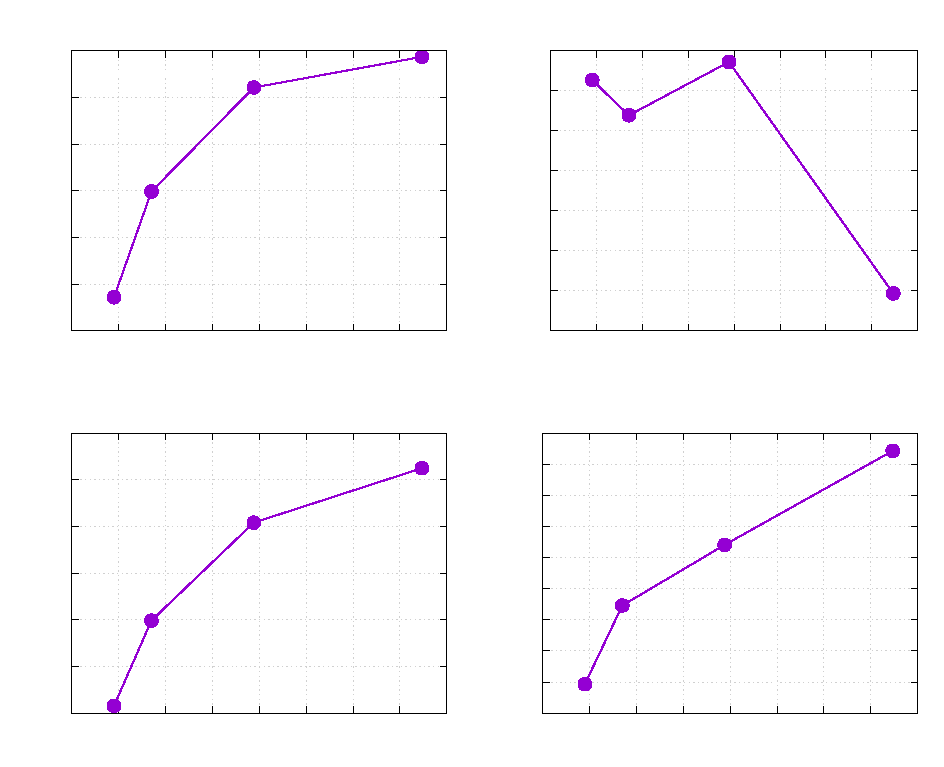
\includegraphics[width={453.00bp},height={368.00bp}]{figures/assignment5_mesh_metrics}}%
    \gplfronttext
  \end{picture}%
\endgroup
}
  \caption{Postoperative mesh-sensitivity metrics as functions of actual volume
  cell count. All meshes use identical geometry, boundary conditions, sampling
  planes, and HXT tetrahedral meshing strategy.}
  \label{fig:mesh_sensitivity}
\end{figure}

\begin{figure}[htbp]
  \centering
  \resizebox{0.98\textwidth}{!}{% GNUPLOT: LaTeX picture with Postscript
\begingroup
  \makeatletter
  \providecommand\color[2][]{%
    \GenericError{(gnuplot) \space\space\space\@spaces}{%
      Package color not loaded in conjunction with
      terminal option `colourtext'%
    }{See the gnuplot documentation for explanation.%
    }{Either use 'blacktext' in gnuplot or load the package
      color.sty in LaTeX.}%
    \renewcommand\color[2][]{}%
  }%
  \providecommand\includegraphics[2][]{%
    \GenericError{(gnuplot) \space\space\space\@spaces}{%
      Package graphicx or graphics not loaded%
    }{See the gnuplot documentation for explanation.%
    }{The gnuplot epslatex terminal needs graphicx.sty or graphics.sty.}%
    \renewcommand\includegraphics[2][]{}%
  }%
  \providecommand\rotatebox[2]{#2}%
  \@ifundefined{ifGPcolor}{%
    \newif\ifGPcolor
    \GPcolortrue
  }{}%
  \@ifundefined{ifGPblacktext}{%
    \newif\ifGPblacktext
    \GPblacktexttrue
  }{}%
  % define a \g@addto@macro without @ in the name:
  \let\gplgaddtomacro\g@addto@macro
  % define empty templates for all commands taking text:
  \gdef\gplbacktext{}%
  \gdef\gplfronttext{}%
  \makeatother
  \ifGPblacktext
    % no textcolor at all
    \def\colorrgb#1{}%
    \def\colorgray#1{}%
  \else
    % gray or color?
    \ifGPcolor
      \def\colorrgb#1{\color[rgb]{#1}}%
      \def\colorgray#1{\color[gray]{#1}}%
      \expandafter\def\csname LTw\endcsname{\color{white}}%
      \expandafter\def\csname LTb\endcsname{\color{black}}%
      \expandafter\def\csname LTa\endcsname{\color{black}}%
      \expandafter\def\csname LT0\endcsname{\color[rgb]{1,0,0}}%
      \expandafter\def\csname LT1\endcsname{\color[rgb]{0,1,0}}%
      \expandafter\def\csname LT2\endcsname{\color[rgb]{0,0,1}}%
      \expandafter\def\csname LT3\endcsname{\color[rgb]{1,0,1}}%
      \expandafter\def\csname LT4\endcsname{\color[rgb]{0,1,1}}%
      \expandafter\def\csname LT5\endcsname{\color[rgb]{1,1,0}}%
      \expandafter\def\csname LT6\endcsname{\color[rgb]{0,0,0}}%
      \expandafter\def\csname LT7\endcsname{\color[rgb]{1,0.3,0}}%
      \expandafter\def\csname LT8\endcsname{\color[rgb]{0.5,0.5,0.5}}%
    \else
      % gray
      \def\colorrgb#1{\color{black}}%
      \def\colorgray#1{\color[gray]{#1}}%
      \expandafter\def\csname LTw\endcsname{\color{white}}%
      \expandafter\def\csname LTb\endcsname{\color{black}}%
      \expandafter\def\csname LTa\endcsname{\color{black}}%
      \expandafter\def\csname LT0\endcsname{\color{black}}%
      \expandafter\def\csname LT1\endcsname{\color{black}}%
      \expandafter\def\csname LT2\endcsname{\color{black}}%
      \expandafter\def\csname LT3\endcsname{\color{black}}%
      \expandafter\def\csname LT4\endcsname{\color{black}}%
      \expandafter\def\csname LT5\endcsname{\color{black}}%
      \expandafter\def\csname LT6\endcsname{\color{black}}%
      \expandafter\def\csname LT7\endcsname{\color{black}}%
      \expandafter\def\csname LT8\endcsname{\color{black}}%
    \fi
  \fi
    \setlength{\unitlength}{0.0500bp}%
    \ifx\gptboxheight\undefined%
      \newlength{\gptboxheight}%
      \newlength{\gptboxwidth}%
      \newsavebox{\gptboxtext}%
    \fi%
    \setlength{\fboxrule}{0.5pt}%
    \setlength{\fboxsep}{1pt}%
    \definecolor{tbcol}{rgb}{1,1,1}%
\begin{picture}(9060.00,7360.00)%
    \gplgaddtomacro\gplbacktext{%
      \csname LTb\endcsname%%
      \put(438,4176){\makebox(0,0)[r]{\strut{}$0$}}%
      \csname LTb\endcsname%%
      \put(438,4512){\makebox(0,0)[r]{\strut{}$2$}}%
      \csname LTb\endcsname%%
      \put(438,4848){\makebox(0,0)[r]{\strut{}$4$}}%
      \csname LTb\endcsname%%
      \put(438,5184){\makebox(0,0)[r]{\strut{}$6$}}%
      \csname LTb\endcsname%%
      \put(438,5520){\makebox(0,0)[r]{\strut{}$8$}}%
      \csname LTb\endcsname%%
      \put(438,5856){\makebox(0,0)[r]{\strut{}$10$}}%
      \csname LTb\endcsname%%
      \put(438,6192){\makebox(0,0)[r]{\strut{}$12$}}%
      \csname LTb\endcsname%%
      \put(438,6528){\makebox(0,0)[r]{\strut{}$14$}}%
      \csname LTb\endcsname%%
      \put(438,6864){\makebox(0,0)[r]{\strut{}$16$}}%
      \csname LTb\endcsname%%
      \put(518,4018){\makebox(0,0){\strut{}0.0$\times10^{0}$}}%
      \csname LTb\endcsname%%
      \put(988,4018){\makebox(0,0){\strut{}2.0$\times10^{5}$}}%
      \csname LTb\endcsname%%
      \put(1459,4018){\makebox(0,0){\strut{}4.0$\times10^{5}$}}%
      \csname LTb\endcsname%%
      \put(1929,4018){\makebox(0,0){\strut{}6.0$\times10^{5}$}}%
      \csname LTb\endcsname%%
      \put(2399,4018){\makebox(0,0){\strut{}8.0$\times10^{5}$}}%
      \csname LTb\endcsname%%
      \put(2869,4018){\makebox(0,0){\strut{}1.0$\times10^{6}$}}%
      \csname LTb\endcsname%%
      \put(3339,4018){\makebox(0,0){\strut{}1.2$\times10^{6}$}}%
      \csname LTb\endcsname%%
      \put(3809,4018){\makebox(0,0){\strut{}1.4$\times10^{6}$}}%
      \csname LTb\endcsname%%
      \put(4279,4018){\makebox(0,0){\strut{}1.6$\times10^{6}$}}%
    }%
    \gplgaddtomacro\gplfronttext{%
      \csname LTb\endcsname%%
      \put(139,5520){\rotatebox{-270.00}{\makebox(0,0){\strut{}Difference from finest mesh (\%)}}}%
      \csname LTb\endcsname%%
      \put(2399,3780){\makebox(0,0){\strut{}Number of volume cells}}%
      \csname LTb\endcsname%%
      \put(2399,7102){\makebox(0,0){\strut{}Resistance (Pa/(L/min))}}%
    }%
    \gplgaddtomacro\gplbacktext{%
      \csname LTb\endcsname%%
      \put(5118,4176){\makebox(0,0)[r]{\strut{}$0$}}%
      \csname LTb\endcsname%%
      \put(5118,4512){\makebox(0,0)[r]{\strut{}$0.05$}}%
      \csname LTb\endcsname%%
      \put(5118,4848){\makebox(0,0)[r]{\strut{}$0.1$}}%
      \csname LTb\endcsname%%
      \put(5118,5184){\makebox(0,0)[r]{\strut{}$0.15$}}%
      \csname LTb\endcsname%%
      \put(5118,5520){\makebox(0,0)[r]{\strut{}$0.2$}}%
      \csname LTb\endcsname%%
      \put(5118,5856){\makebox(0,0)[r]{\strut{}$0.25$}}%
      \csname LTb\endcsname%%
      \put(5118,6192){\makebox(0,0)[r]{\strut{}$0.3$}}%
      \csname LTb\endcsname%%
      \put(5118,6528){\makebox(0,0)[r]{\strut{}$0.35$}}%
      \csname LTb\endcsname%%
      \put(5118,6864){\makebox(0,0)[r]{\strut{}$0.4$}}%
      \csname LTb\endcsname%%
      \put(5199,4018){\makebox(0,0){\strut{}0.0$\times10^{0}$}}%
      \csname LTb\endcsname%%
      \put(5649,4018){\makebox(0,0){\strut{}2.0$\times10^{5}$}}%
      \csname LTb\endcsname%%
      \put(6099,4018){\makebox(0,0){\strut{}4.0$\times10^{5}$}}%
      \csname LTb\endcsname%%
      \put(6549,4018){\makebox(0,0){\strut{}6.0$\times10^{5}$}}%
      \csname LTb\endcsname%%
      \put(6999,4018){\makebox(0,0){\strut{}8.0$\times10^{5}$}}%
      \csname LTb\endcsname%%
      \put(7449,4018){\makebox(0,0){\strut{}1.0$\times10^{6}$}}%
      \csname LTb\endcsname%%
      \put(7899,4018){\makebox(0,0){\strut{}1.2$\times10^{6}$}}%
      \csname LTb\endcsname%%
      \put(8349,4018){\makebox(0,0){\strut{}1.4$\times10^{6}$}}%
      \csname LTb\endcsname%%
      \put(8799,4018){\makebox(0,0){\strut{}1.6$\times10^{6}$}}%
    }%
    \gplgaddtomacro\gplfronttext{%
      \csname LTb\endcsname%%
      \put(4659,5520){\rotatebox{-270.00}{\makebox(0,0){\strut{}Difference from finest mesh (\%)}}}%
      \csname LTb\endcsname%%
      \put(6999,3780){\makebox(0,0){\strut{}Number of volume cells}}%
      \csname LTb\endcsname%%
      \put(6999,7102){\makebox(0,0){\strut{}Right-lung flow fraction (\%)}}%
    }%
    \gplgaddtomacro\gplbacktext{%
      \csname LTb\endcsname%%
      \put(358,506){\makebox(0,0)[r]{\strut{}$0$}}%
      \csname LTb\endcsname%%
      \put(358,890){\makebox(0,0)[r]{\strut{}$1$}}%
      \csname LTb\endcsname%%
      \put(358,1274){\makebox(0,0)[r]{\strut{}$2$}}%
      \csname LTb\endcsname%%
      \put(358,1658){\makebox(0,0)[r]{\strut{}$3$}}%
      \csname LTb\endcsname%%
      \put(358,2042){\makebox(0,0)[r]{\strut{}$4$}}%
      \csname LTb\endcsname%%
      \put(358,2426){\makebox(0,0)[r]{\strut{}$5$}}%
      \csname LTb\endcsname%%
      \put(358,2810){\makebox(0,0)[r]{\strut{}$6$}}%
      \csname LTb\endcsname%%
      \put(358,3194){\makebox(0,0)[r]{\strut{}$7$}}%
      \csname LTb\endcsname%%
      \put(438,348){\makebox(0,0){\strut{}0.0$\times10^{0}$}}%
      \csname LTb\endcsname%%
      \put(918,348){\makebox(0,0){\strut{}2.0$\times10^{5}$}}%
      \csname LTb\endcsname%%
      \put(1398,348){\makebox(0,0){\strut{}4.0$\times10^{5}$}}%
      \csname LTb\endcsname%%
      \put(1879,348){\makebox(0,0){\strut{}6.0$\times10^{5}$}}%
      \csname LTb\endcsname%%
      \put(2359,348){\makebox(0,0){\strut{}8.0$\times10^{5}$}}%
      \csname LTb\endcsname%%
      \put(2839,348){\makebox(0,0){\strut{}1.0$\times10^{6}$}}%
      \csname LTb\endcsname%%
      \put(3319,348){\makebox(0,0){\strut{}1.2$\times10^{6}$}}%
      \csname LTb\endcsname%%
      \put(3799,348){\makebox(0,0){\strut{}1.4$\times10^{6}$}}%
      \csname LTb\endcsname%%
      \put(4279,348){\makebox(0,0){\strut{}1.6$\times10^{6}$}}%
    }%
    \gplgaddtomacro\gplfronttext{%
      \csname LTb\endcsname%%
      \put(139,1850){\rotatebox{-270.00}{\makebox(0,0){\strut{}Difference from finest mesh (\%)}}}%
      \csname LTb\endcsname%%
      \put(2359,110){\makebox(0,0){\strut{}Number of volume cells}}%
      \csname LTb\endcsname%%
      \put(2359,3432){\makebox(0,0){\strut{}Right-superior share of right flow (\%)}}%
    }%
    \gplgaddtomacro\gplbacktext{%
      \csname LTb\endcsname%%
      \put(5038,506){\makebox(0,0)[r]{\strut{}$0$}}%
      \csname LTb\endcsname%%
      \put(5038,842){\makebox(0,0)[r]{\strut{}$0.5$}}%
      \csname LTb\endcsname%%
      \put(5038,1178){\makebox(0,0)[r]{\strut{}$1$}}%
      \csname LTb\endcsname%%
      \put(5038,1514){\makebox(0,0)[r]{\strut{}$1.5$}}%
      \csname LTb\endcsname%%
      \put(5038,1850){\makebox(0,0)[r]{\strut{}$2$}}%
      \csname LTb\endcsname%%
      \put(5038,2186){\makebox(0,0)[r]{\strut{}$2.5$}}%
      \csname LTb\endcsname%%
      \put(5038,2522){\makebox(0,0)[r]{\strut{}$3$}}%
      \csname LTb\endcsname%%
      \put(5038,2858){\makebox(0,0)[r]{\strut{}$3.5$}}%
      \csname LTb\endcsname%%
      \put(5038,3194){\makebox(0,0)[r]{\strut{}$4$}}%
      \csname LTb\endcsname%%
      \put(5118,348){\makebox(0,0){\strut{}0.0$\times10^{0}$}}%
      \csname LTb\endcsname%%
      \put(5579,348){\makebox(0,0){\strut{}2.0$\times10^{5}$}}%
      \csname LTb\endcsname%%
      \put(6039,348){\makebox(0,0){\strut{}4.0$\times10^{5}$}}%
      \csname LTb\endcsname%%
      \put(6499,348){\makebox(0,0){\strut{}6.0$\times10^{5}$}}%
      \csname LTb\endcsname%%
      \put(6959,348){\makebox(0,0){\strut{}8.0$\times10^{5}$}}%
      \csname LTb\endcsname%%
      \put(7419,348){\makebox(0,0){\strut{}1.0$\times10^{6}$}}%
      \csname LTb\endcsname%%
      \put(7879,348){\makebox(0,0){\strut{}1.2$\times10^{6}$}}%
      \csname LTb\endcsname%%
      \put(8339,348){\makebox(0,0){\strut{}1.4$\times10^{6}$}}%
      \csname LTb\endcsname%%
      \put(8799,348){\makebox(0,0){\strut{}1.6$\times10^{6}$}}%
    }%
    \gplgaddtomacro\gplfronttext{%
      \csname LTb\endcsname%%
      \put(4659,1850){\rotatebox{-270.00}{\makebox(0,0){\strut{}Difference from finest mesh (\%)}}}%
      \csname LTb\endcsname%%
      \put(6959,110){\makebox(0,0){\strut{}Number of volume cells}}%
      \csname LTb\endcsname%%
      \put(6959,3432){\makebox(0,0){\strut{}Matched-section peak velocity (m/s)}}%
    }%
    \gplbacktext
    \put(0,0){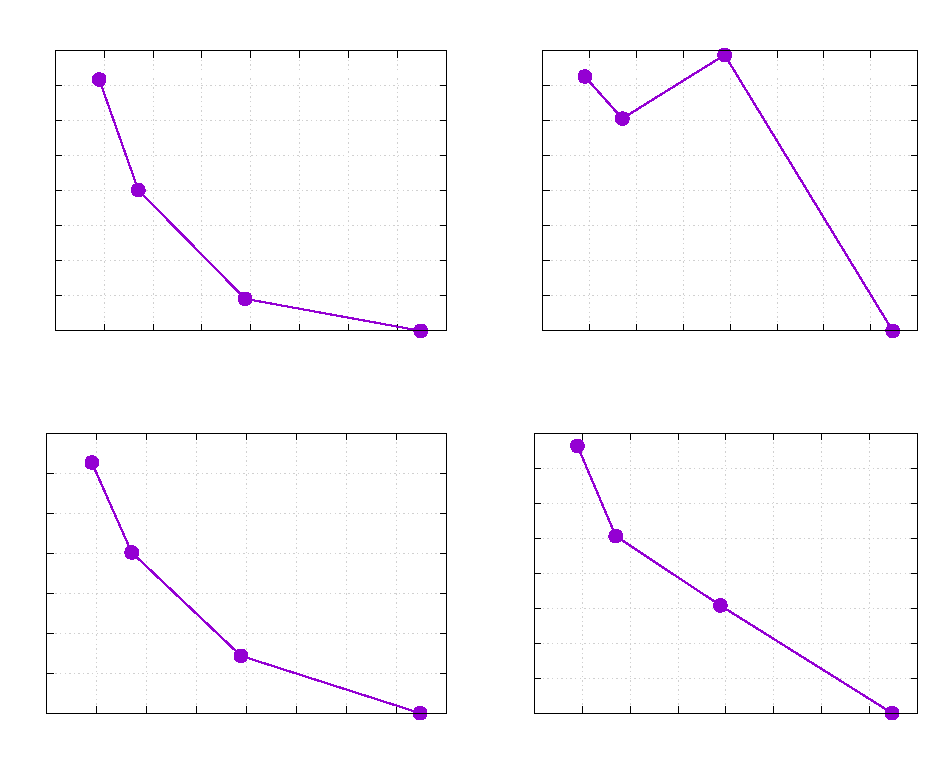
\includegraphics[width={453.00bp},height={368.00bp}]{figures/assignment5_mesh_differences}}%
    \gplfronttext
  \end{picture}%
\endgroup
}
  \caption{Absolute relative differences from the densest 0.12 mm mesh,
  calculated as $|\phi_i-\phi_d|/|\phi_d|\times100\%$. The densest case reached
  its 2000-iteration limit without satisfying residual control and is therefore
  a requested comparison rather than an accepted truth solution.}
  \label{fig:mesh_sensitivity_differences}
\end{figure}

% -----------------------------------------------------------------------------
\section{Results}
\label{sec:results}

\subsection{Velocity field}

At the converged postoperative solution, velocity vectors accelerate through the
narrow distal trachea and divide at the carina. The fixed matched section has an
area-averaged axial velocity of \SI{6.53}{\metre\per\second} and a sectional
peak magnitude of \SI{9.25}{\metre\per\second}. The vectors also show the
unequal right/left flow division quantified from patch fluxes.

\begin{figure}[htbp]
  \centering
  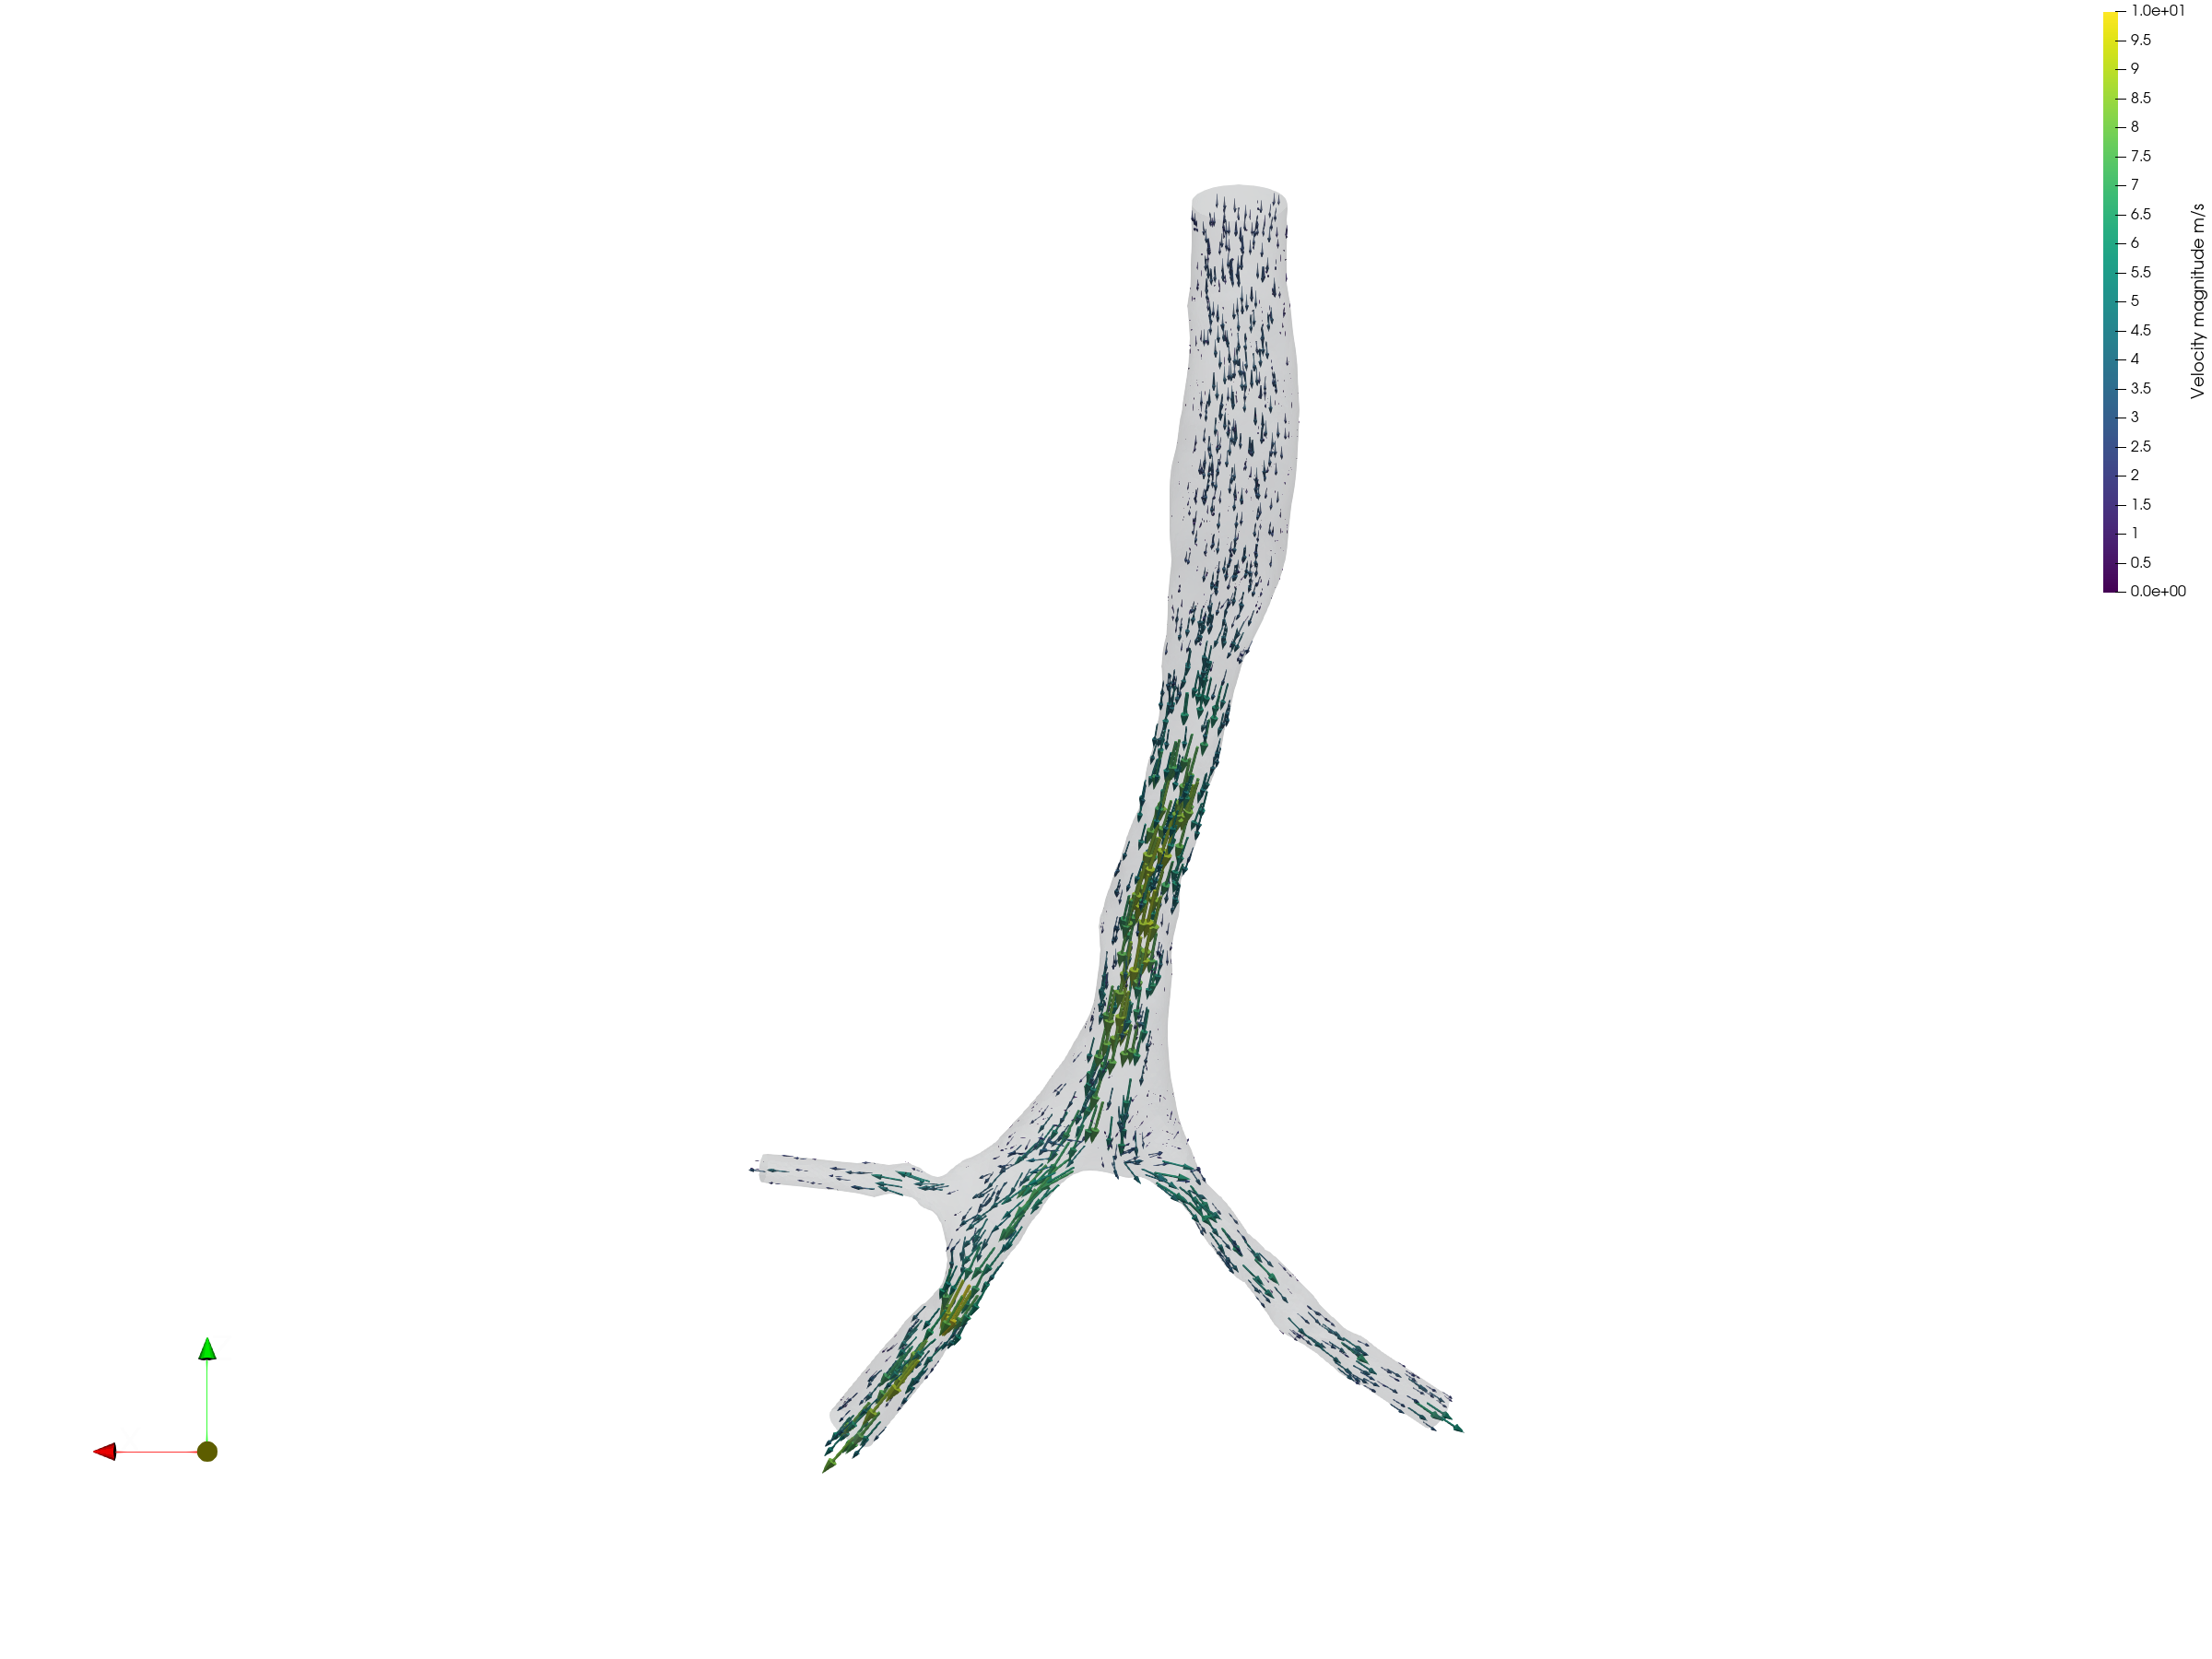
\includegraphics[width=0.92\textwidth]{assignment4_velocity_vectors.png}
  \caption{Postoperative velocity-vector field at the converged steady solution
  (iteration 589). Arrow direction represents local flow direction; arrow colour
  represents velocity magnitude on a fixed \SIrange{0}{10}{\metre\per\second}
  scale. The airway surface is shown semi-transparently for anatomical context.}
  \label{fig:velocity}
\end{figure}

\subsection{Pressure distribution}

Pressure is reported relative to the zero-gauge-pressure outlets and converted
from OpenFOAM kinematic pressure using $P=\rho p$ with
$\rho=\SI{1.204}{\kilogram\per\metre\cubed}$. Pressure decreases from the
tracheal inlet toward the outlets. Along the mapped centerline interval it falls
from approximately \SI{65.1}{\pascal} to \SI{34.1}{\pascal}, with a local
minimum followed by partial recovery. The resistance calculation uses
area-averaged plane pressures rather than centerline point samples.

\begin{figure}[htbp]
  \centering
  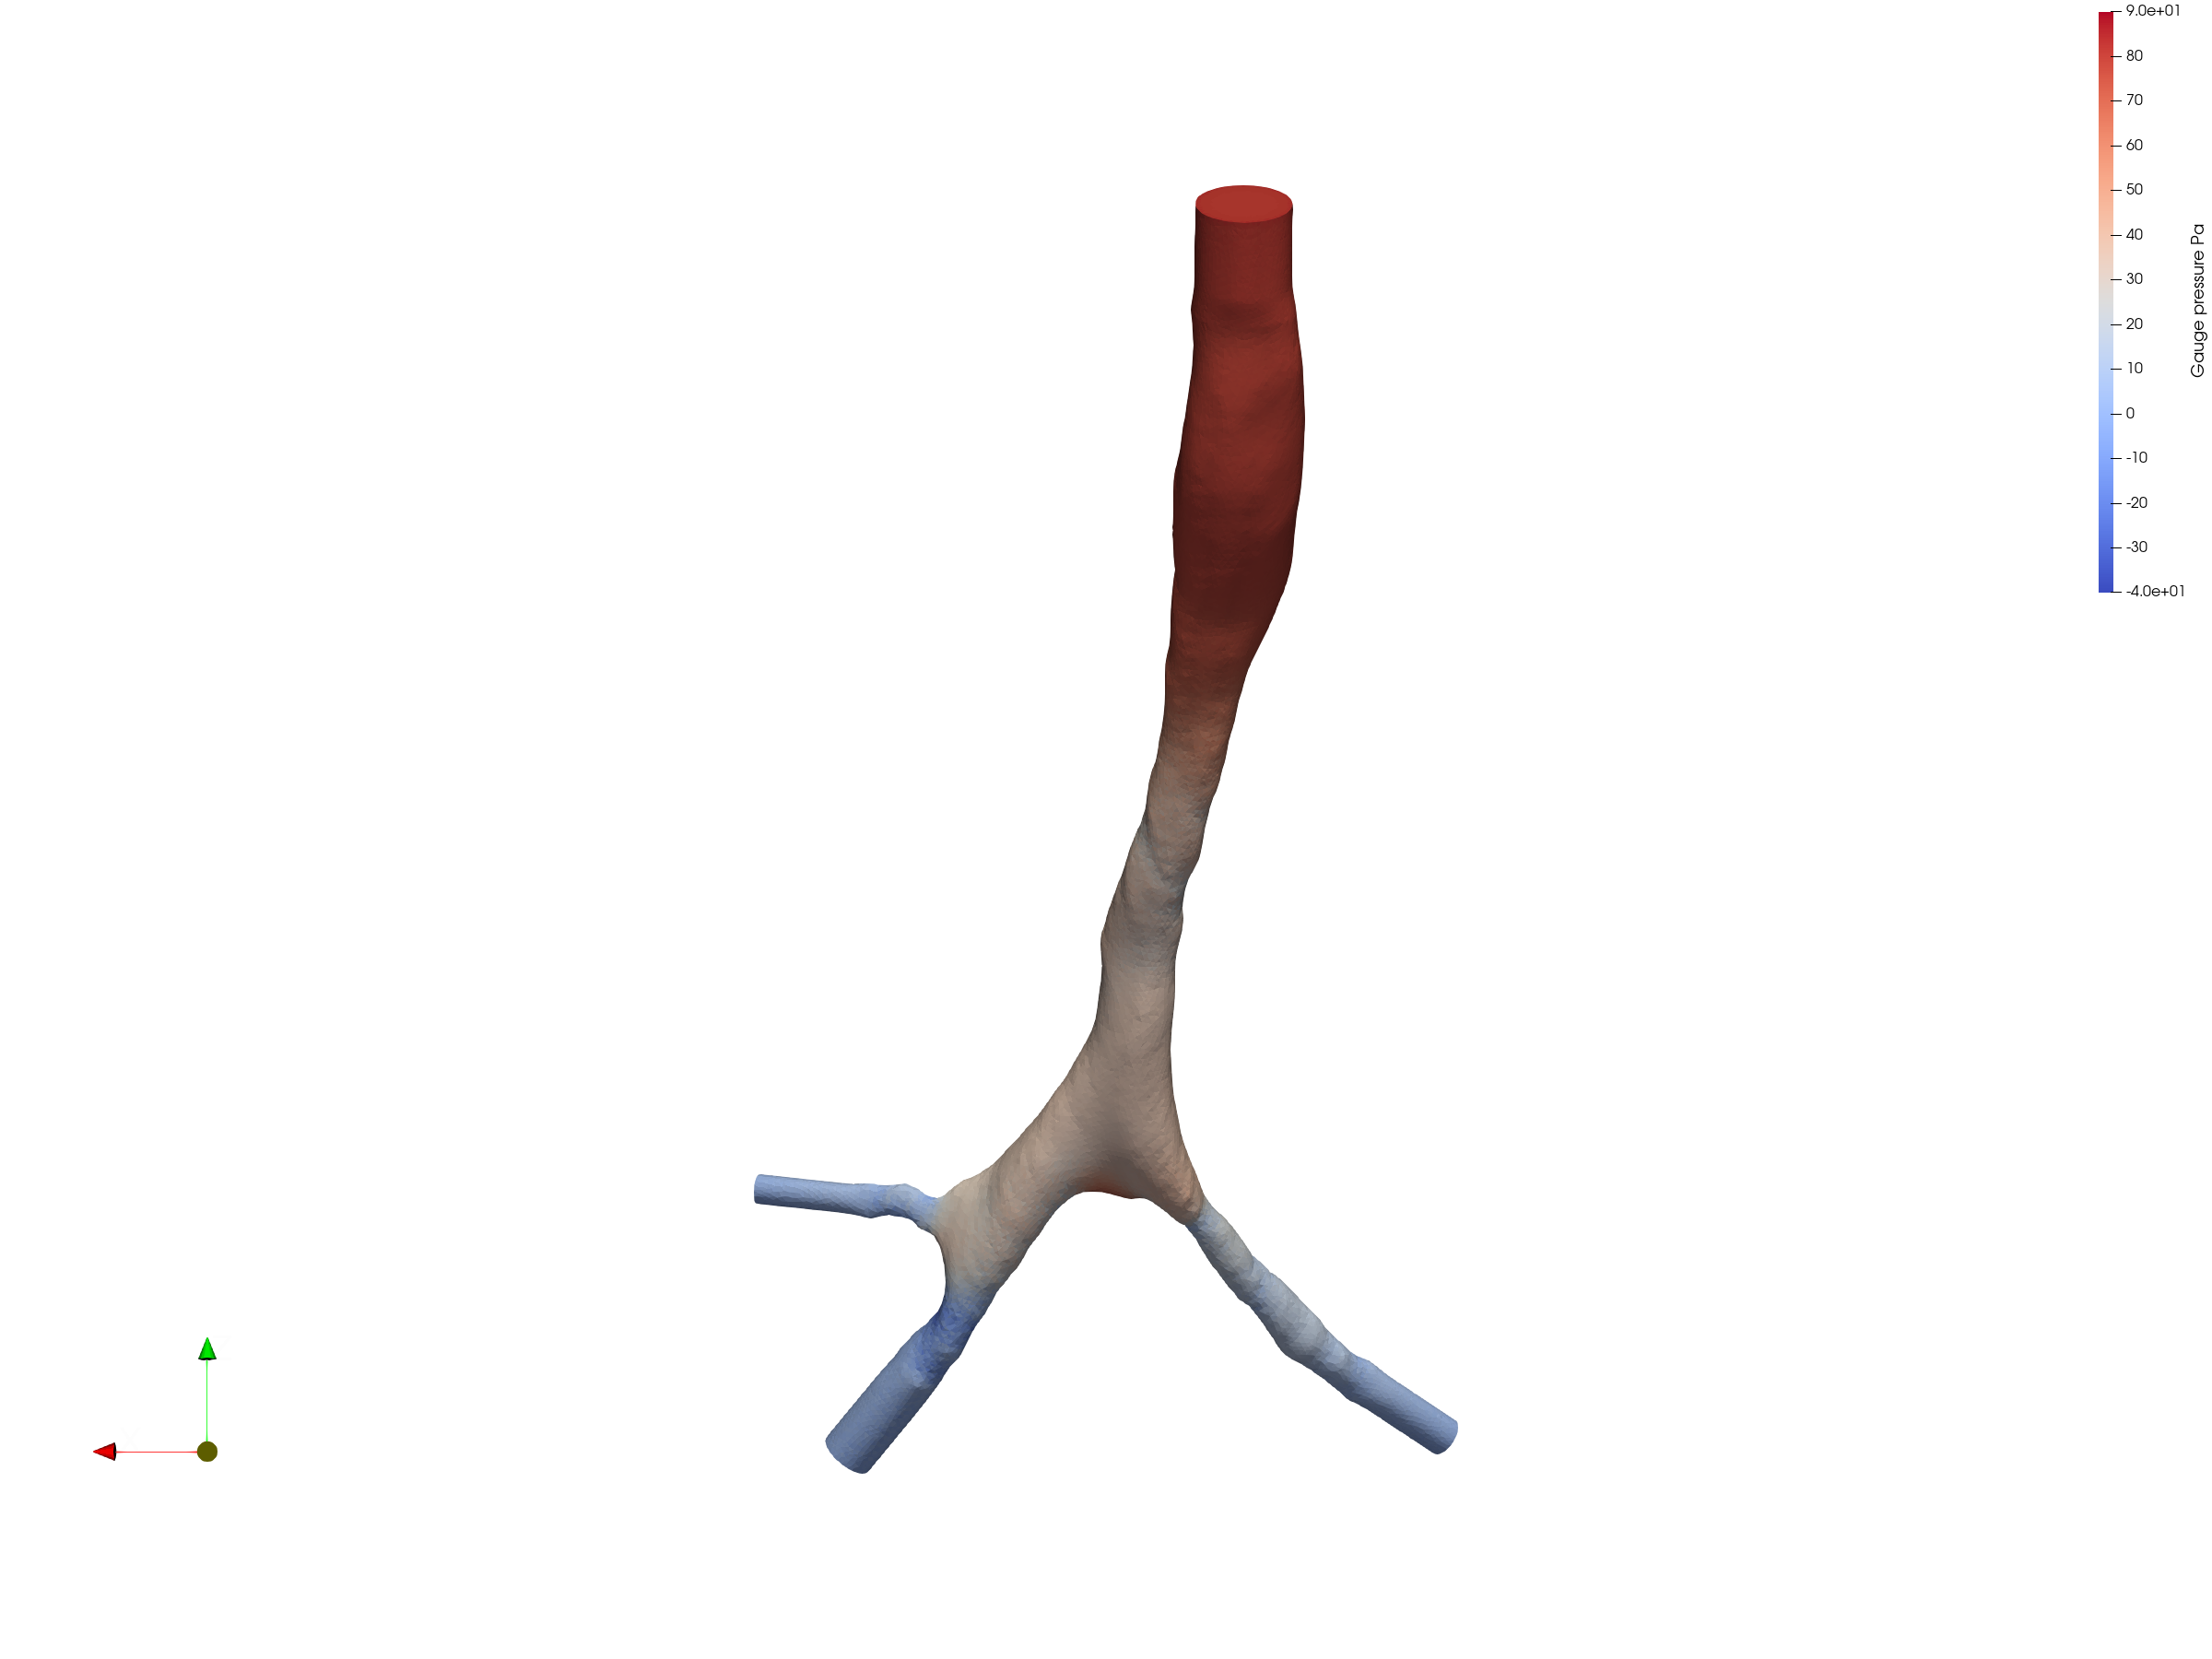
\includegraphics[width=0.92\textwidth]{assignment4_pressure_distribution.png}
  \caption{Postoperative dimensional gauge-pressure distribution at the
  converged steady solution (iteration 589), shown in anatomical frontal view.
  OpenFOAM kinematic pressure was multiplied by an air density of
  \SI{1.204}{\kilogram\per\metre\cubed}; outlet gauge pressure is zero.}
  \label{fig:pressure}
\end{figure}

\begin{figure}[htbp]
  \centering
  \resizebox{0.95\textwidth}{!}{% GNUPLOT: LaTeX picture with Postscript
\begingroup
  \makeatletter
  \providecommand\color[2][]{%
    \GenericError{(gnuplot) \space\space\space\@spaces}{%
      Package color not loaded in conjunction with
      terminal option `colourtext'%
    }{See the gnuplot documentation for explanation.%
    }{Either use 'blacktext' in gnuplot or load the package
      color.sty in LaTeX.}%
    \renewcommand\color[2][]{}%
  }%
  \providecommand\includegraphics[2][]{%
    \GenericError{(gnuplot) \space\space\space\@spaces}{%
      Package graphicx or graphics not loaded%
    }{See the gnuplot documentation for explanation.%
    }{The gnuplot epslatex terminal needs graphicx.sty or graphics.sty.}%
    \renewcommand\includegraphics[2][]{}%
  }%
  \providecommand\rotatebox[2]{#2}%
  \@ifundefined{ifGPcolor}{%
    \newif\ifGPcolor
    \GPcolortrue
  }{}%
  \@ifundefined{ifGPblacktext}{%
    \newif\ifGPblacktext
    \GPblacktexttrue
  }{}%
  % define a \g@addto@macro without @ in the name:
  \let\gplgaddtomacro\g@addto@macro
  % define empty templates for all commands taking text:
  \gdef\gplbacktext{}%
  \gdef\gplfronttext{}%
  \makeatother
  \ifGPblacktext
    % no textcolor at all
    \def\colorrgb#1{}%
    \def\colorgray#1{}%
  \else
    % gray or color?
    \ifGPcolor
      \def\colorrgb#1{\color[rgb]{#1}}%
      \def\colorgray#1{\color[gray]{#1}}%
      \expandafter\def\csname LTw\endcsname{\color{white}}%
      \expandafter\def\csname LTb\endcsname{\color{black}}%
      \expandafter\def\csname LTa\endcsname{\color{black}}%
      \expandafter\def\csname LT0\endcsname{\color[rgb]{1,0,0}}%
      \expandafter\def\csname LT1\endcsname{\color[rgb]{0,1,0}}%
      \expandafter\def\csname LT2\endcsname{\color[rgb]{0,0,1}}%
      \expandafter\def\csname LT3\endcsname{\color[rgb]{1,0,1}}%
      \expandafter\def\csname LT4\endcsname{\color[rgb]{0,1,1}}%
      \expandafter\def\csname LT5\endcsname{\color[rgb]{1,1,0}}%
      \expandafter\def\csname LT6\endcsname{\color[rgb]{0,0,0}}%
      \expandafter\def\csname LT7\endcsname{\color[rgb]{1,0.3,0}}%
      \expandafter\def\csname LT8\endcsname{\color[rgb]{0.5,0.5,0.5}}%
    \else
      % gray
      \def\colorrgb#1{\color{black}}%
      \def\colorgray#1{\color[gray]{#1}}%
      \expandafter\def\csname LTw\endcsname{\color{white}}%
      \expandafter\def\csname LTb\endcsname{\color{black}}%
      \expandafter\def\csname LTa\endcsname{\color{black}}%
      \expandafter\def\csname LT0\endcsname{\color{black}}%
      \expandafter\def\csname LT1\endcsname{\color{black}}%
      \expandafter\def\csname LT2\endcsname{\color{black}}%
      \expandafter\def\csname LT3\endcsname{\color{black}}%
      \expandafter\def\csname LT4\endcsname{\color{black}}%
      \expandafter\def\csname LT5\endcsname{\color{black}}%
      \expandafter\def\csname LT6\endcsname{\color{black}}%
      \expandafter\def\csname LT7\endcsname{\color{black}}%
      \expandafter\def\csname LT8\endcsname{\color{black}}%
    \fi
  \fi
    \setlength{\unitlength}{0.0500bp}%
    \ifx\gptboxheight\undefined%
      \newlength{\gptboxheight}%
      \newlength{\gptboxwidth}%
      \newsavebox{\gptboxtext}%
    \fi%
    \setlength{\fboxrule}{0.5pt}%
    \setlength{\fboxsep}{1pt}%
    \definecolor{tbcol}{rgb}{1,1,1}%
\begin{picture}(8500.00,4800.00)%
    \gplgaddtomacro\gplbacktext{%
      \csname LTb\endcsname%%
      \put(487,562){\makebox(0,0)[r]{\strut{}$40$}}%
      \csname LTb\endcsname%%
      \put(487,1024){\makebox(0,0)[r]{\strut{}$45$}}%
      \csname LTb\endcsname%%
      \put(487,1485){\makebox(0,0)[r]{\strut{}$50$}}%
      \csname LTb\endcsname%%
      \put(487,1946){\makebox(0,0)[r]{\strut{}$55$}}%
      \csname LTb\endcsname%%
      \put(487,2407){\makebox(0,0)[r]{\strut{}$60$}}%
      \csname LTb\endcsname%%
      \put(487,2868){\makebox(0,0)[r]{\strut{}$65$}}%
      \csname LTb\endcsname%%
      \put(487,3329){\makebox(0,0)[r]{\strut{}$70$}}%
      \csname LTb\endcsname%%
      \put(487,3791){\makebox(0,0)[r]{\strut{}$75$}}%
      \csname LTb\endcsname%%
      \put(487,4252){\makebox(0,0)[r]{\strut{}$80$}}%
      \csname LTb\endcsname%%
      \put(576,386){\makebox(0,0){\strut{}$0$}}%
      \csname LTb\endcsname%%
      \put(1667,386){\makebox(0,0){\strut{}$2$}}%
      \csname LTb\endcsname%%
      \put(2758,386){\makebox(0,0){\strut{}$4$}}%
      \csname LTb\endcsname%%
      \put(3849,386){\makebox(0,0){\strut{}$6$}}%
      \csname LTb\endcsname%%
      \put(4940,386){\makebox(0,0){\strut{}$8$}}%
      \csname LTb\endcsname%%
      \put(6031,386){\makebox(0,0){\strut{}$10$}}%
      \csname LTb\endcsname%%
      \put(7122,386){\makebox(0,0){\strut{}$12$}}%
      \csname LTb\endcsname%%
      \put(8212,386){\makebox(0,0){\strut{}$14$}}%
    }%
    \gplgaddtomacro\gplfronttext{%
      \csname LTb\endcsname%%
      \put(154,2407){\rotatebox{-270.00}{\makebox(0,0){\strut{}Area-interpolated centerline pressure (Pa)}}}%
      \csname LTb\endcsname%%
      \put(4394,123){\makebox(0,0){\strut{}Centerline distance from mapped superior limit (mm)}}%
      \csname LTb\endcsname%%
      \put(4394,4516){\makebox(0,0){\strut{}Postoperative pressure through the anatomically matched region}}%
    }%
    \gplbacktext
    \put(0,0){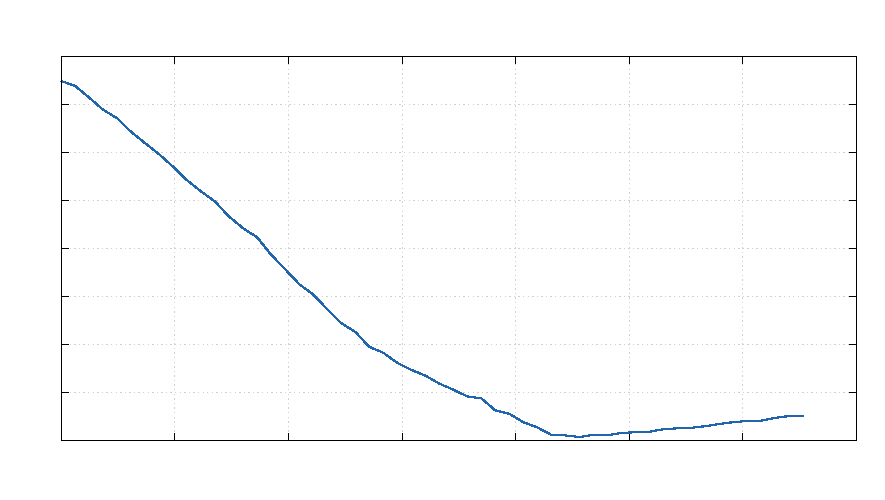
\includegraphics[width={425.00bp},height={240.00bp}]{figures/assignment4_centerline_pressure}}%
    \gplfronttext
  \end{picture}%
\endgroup
}
  \caption{Centerline-interpolated dimensional pressure across the postoperative
  region corresponding to the preoperative stenosis. Distance is measured from
  the mapped superior limit toward the mapped inferior limit. This profile shows
  local pressure evolution; resistance is calculated separately from
  area-averaged pressures on the bounding planes.}
  \label{fig:centerline_pressure}
\end{figure}

\subsection{Outlet and lung flow distribution}

Outlet flow was obtained by integrating outward-normal volumetric flux over each
patch. The right superior and inferior lobar outlets were grouped as the right
lung; the left main bronchus formed the left group. The primary left/right result
was

\begin{equation}
  Q_R = 73.17\%, \qquad Q_L = 26.83\%.
\end{equation}

The individual outlet values in Table~\ref{tab:outlet_flow} provide the supporting
lobar decomposition. Because identical zero gauge pressure was imposed at all
outlets, no 73/27 split was prescribed. The unequal distribution instead reflects
the geometric and hydraulic resistance of the branches resolved within the
truncated airway domain.

\begin{table}[htbp]
  \centering
  \caption{Outlet flow rates and fractions.}
  \label{tab:outlet_flow}
  \begin{tabular}{@{}lrrrr@{}}
    \toprule
    Case & Outlet 1 (\%) & Outlet 2 (\%) & Outlet 3 (\%) & Imbalance (\%) \\
    \midrule
    Postoperative & 11.23 & 61.94 & 26.83 & $6.0\times10^{-7}$ \\
    \bottomrule
  \end{tabular}
\end{table}

\begin{table}[htbp]
  \centering
  \caption{Postoperative left/right lung flow distribution.}
  \label{tab:lung_flow}
  \begin{tabular}{@{}lrr@{}}
    \toprule
    Lung & Flow rate (\si{\metre\cubed\per\second}) & Fraction (\%) \\
    \midrule
    Left  & $8.9449\times10^{-6}$ & 26.83 \\
    Right & $2.4388\times10^{-5}$ & 73.17 \\
    \bottomrule
  \end{tabular}
\end{table}

\subsection{Local resistance before the bifurcation}
\label{sec:steady_resistance}

Two planes normal to the centerline delimit a fixed section before the
bifurcation, corresponding approximately to the location of the preoperative
constriction. These same plane definitions are reused for every mesh and for the
transient Assignment 6 analysis. With dimensional pressure difference
$\Delta P$ and volumetric flow $Q$, local resistance is

\begin{equation}
  R(t)=\frac{\overline{P}_{\mathrm{up}}(t)-
  \overline{P}_{\mathrm{down}}(t)}{Q(t)}.
  \label{eq:local_resistance}
\end{equation}

For the incompressible OpenFOAM pressure field $p$,
$\Delta P=\rho\,\Delta p$. Area-averaged kinematic pressures were
\SI{53.70}{\metre\squared\per\second\squared} upstream and
\SI{27.99}{\metre\squared\per\second\squared} downstream. With
$\rho=\SI{1.204}{\kilogram\per\metre\cubed}$, the local pressure drop was
\SI{30.95}{\pascal}; at $Q=\SI{3.347e-5}{\metre\cubed\per\second}$ this gives
$R=\SI{9.25e5}{\pascal\second\per\metre\cubed}$, equivalent to
\SI{15.41}{\pascal\per\litre\per\minute}. The matched-plane mean axial and peak
velocities were \SI{6.53}{\metre\per\second} and
\SI{9.25}{\metre\per\second}, respectively.

\begin{figure}[htbp]
  \centering
  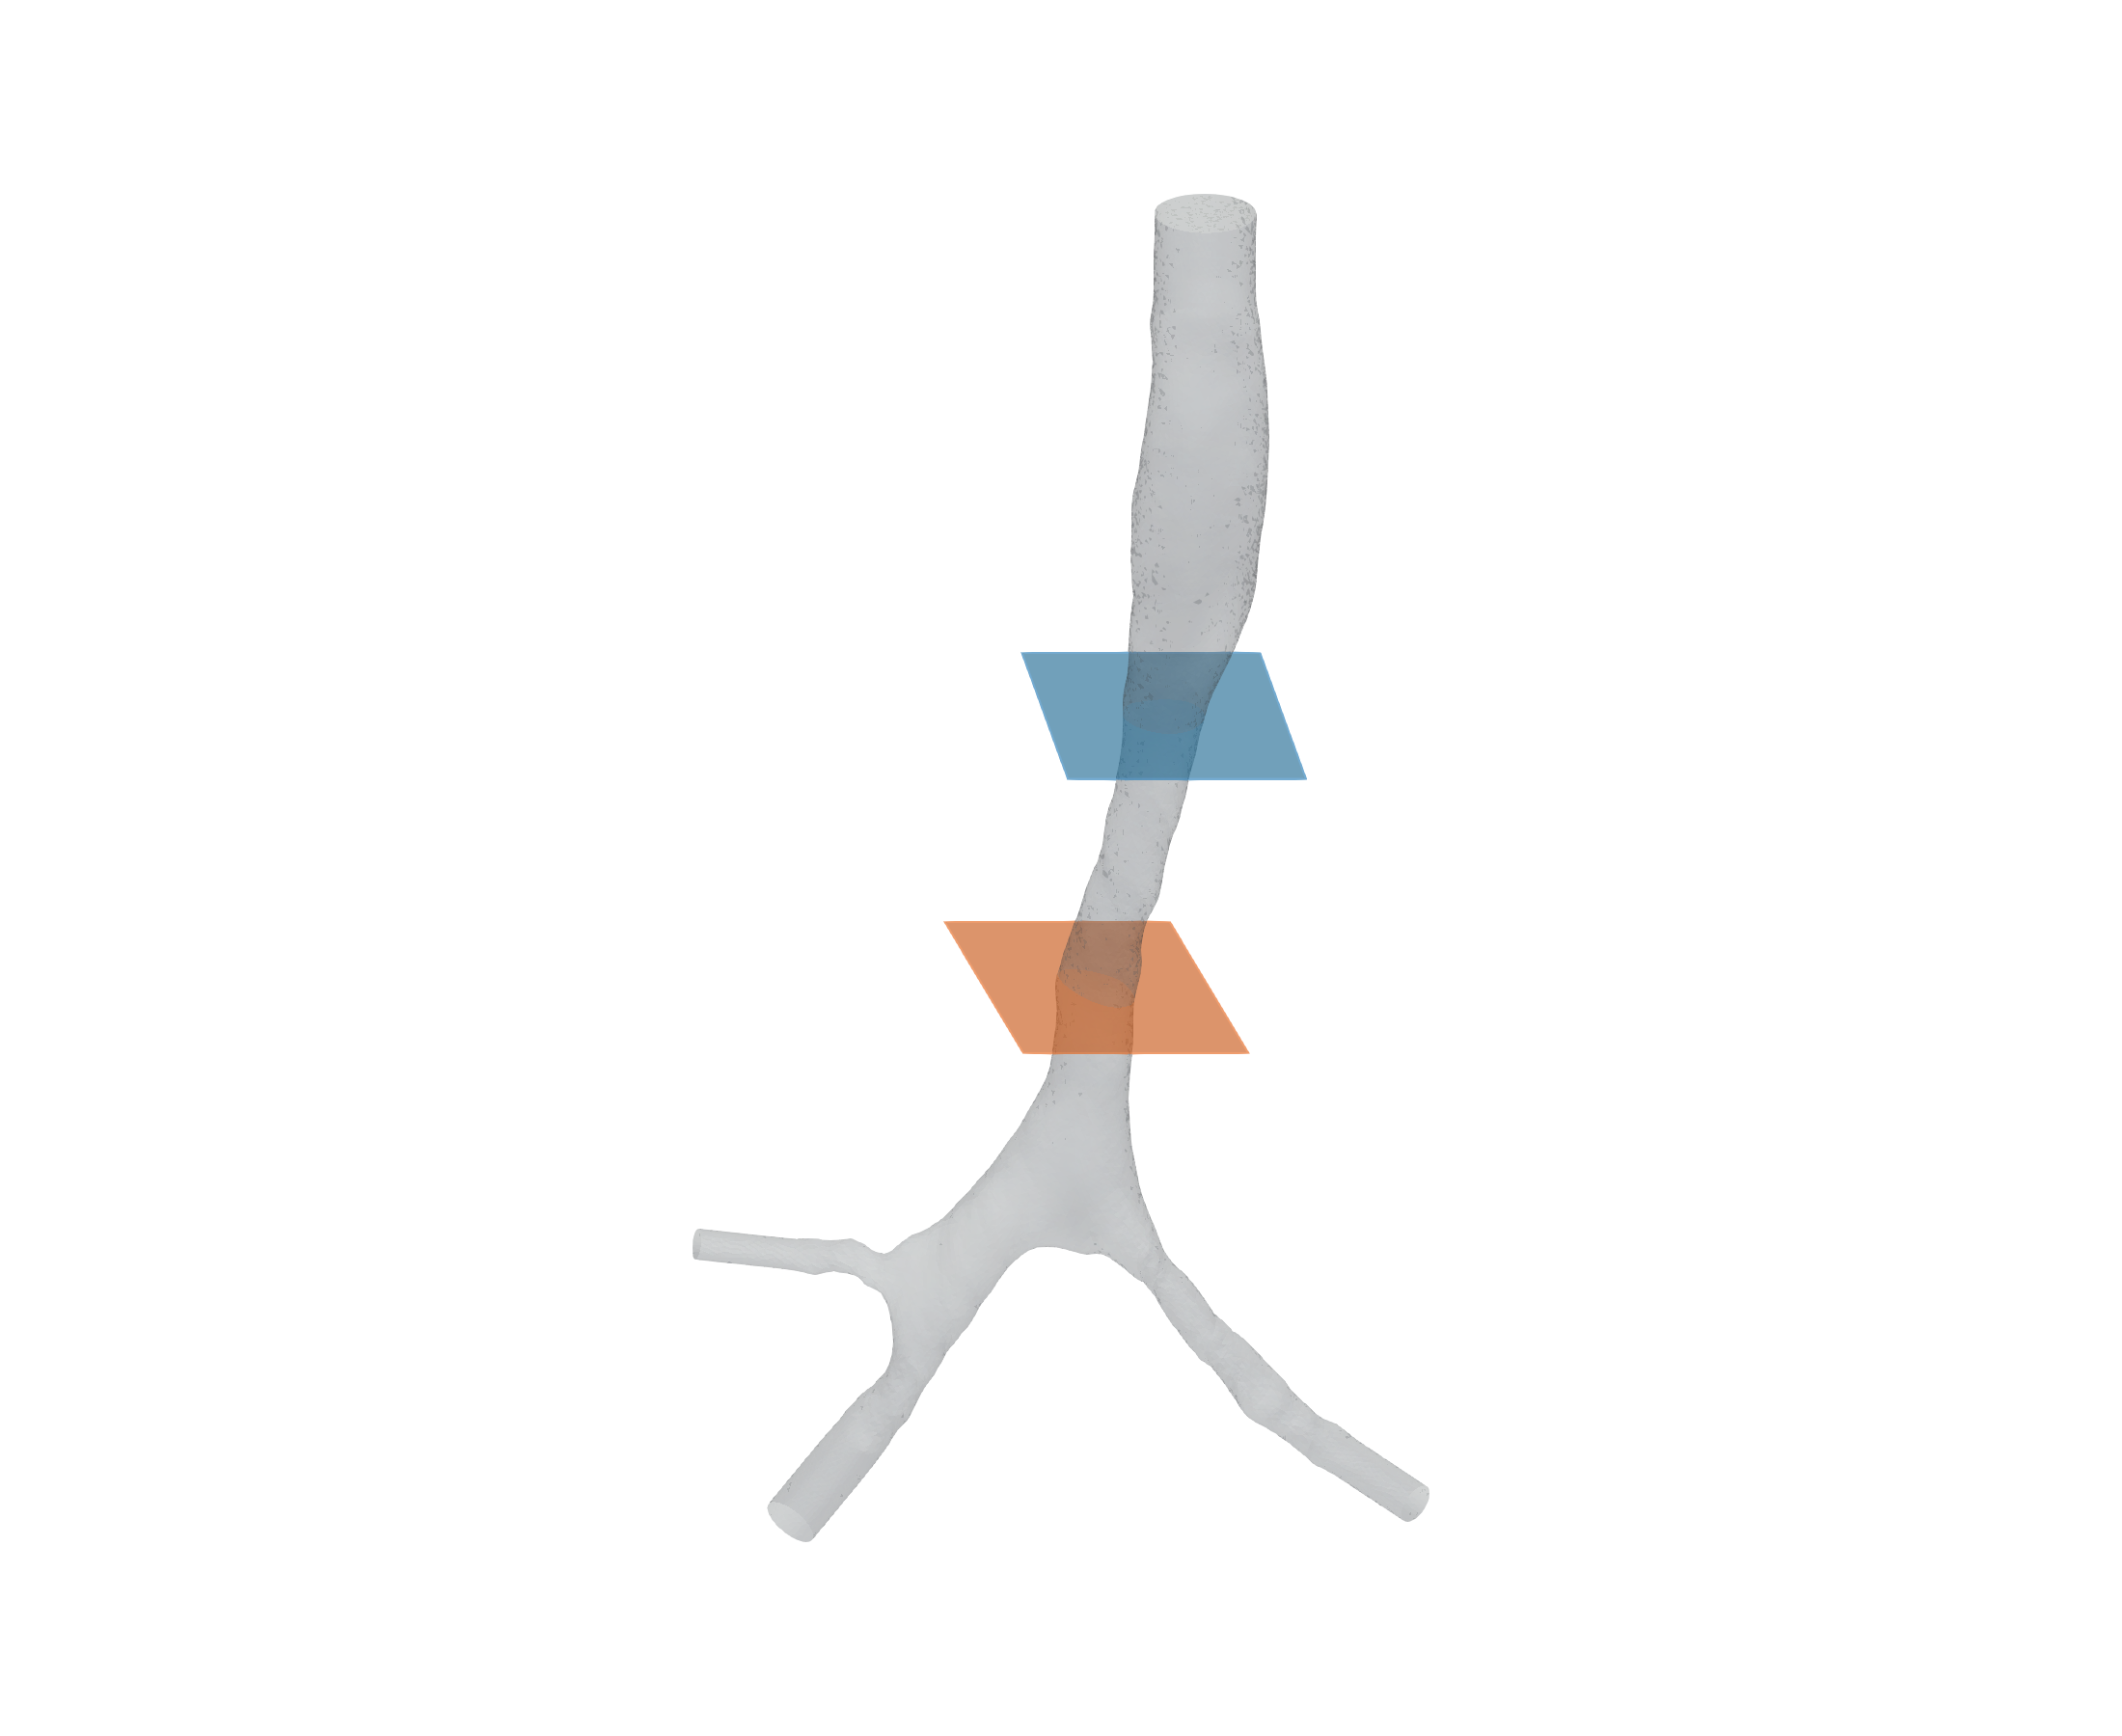
\includegraphics[width=0.76\textwidth]{assignment4_resistance_planes.png}
  \caption{Fixed centerline-normal planes delimiting the postoperative matched
  tracheal region. The blue superior plane is the upstream pressure section and
  the orange inferior plane is the downstream section. Their origins and normals
  are archived in a versioned JSON definition and reused unchanged for steady,
  mesh-sensitivity, and transient analyses.}
  \label{fig:resistance_section}
\end{figure}

\begin{table}[htbp]
  \centering
  \caption{Steady postoperative local-resistance calculation.}
  \label{tab:steady_resistance}
  \begin{tabular}{@{}lr@{}}
    \toprule
    Quantity & Value \\
    \midrule
    Upstream area-averaged kinematic pressure & 53.695 \si{\metre\squared\per\second\squared} \\
    Downstream area-averaged kinematic pressure & 27.993 \si{\metre\squared\per\second\squared} \\
    Pressure difference $\Delta P$ & 30.945 \si{\pascal} \\
    Volumetric flow $Q$ & \num{3.347e-5} \si{\metre\cubed\per\second} \\
    Resistance $R=\Delta P/Q$ & \num{9.247e5} \si{\pascal\second\per\metre\cubed} \\
    \bottomrule
  \end{tabular}
\end{table}

% -----------------------------------------------------------------------------
\section{Transient postoperative analysis}
\label{sec:transient_results}

\subsection{Time-step convergence}

The complete cycle comprised 355,016 adaptive timesteps. Of these, 354,399
(99.826\%) satisfied the PIMPLE outer criterion and 617 reached the limit of
three correctors. The latter were localized around zero-flow transitions: 180
near startup, 309 around the inspiration--expiration reversal at
$t=\SI{1}{\second}$, and 128 near cycle end; no failures occurred over the main
high-flow intervals. The maximum Courant number was 5.296 and the mean Courant
number never exceeded 0.540. The timestep varied from
\SI{3.287e-6}{\second} to \SI{2.019e-4}{\second}. Final equation residuals were
typically of order $10^{-9}$, while the maximum absolute cumulative continuity
error was $5.25\times10^{-4}$. Thus the run remained bounded and predominantly
converged, but reversal-adjacent states and precise transient extrema are
interpreted cautiously.

\begin{figure}[htbp]
  \centering
  \resizebox{0.92\textwidth}{!}{% GNUPLOT: LaTeX picture with Postscript
\begingroup
  \makeatletter
  \providecommand\color[2][]{%
    \GenericError{(gnuplot) \space\space\space\@spaces}{%
      Package color not loaded in conjunction with
      terminal option `colourtext'%
    }{See the gnuplot documentation for explanation.%
    }{Either use 'blacktext' in gnuplot or load the package
      color.sty in LaTeX.}%
    \renewcommand\color[2][]{}%
  }%
  \providecommand\includegraphics[2][]{%
    \GenericError{(gnuplot) \space\space\space\@spaces}{%
      Package graphicx or graphics not loaded%
    }{See the gnuplot documentation for explanation.%
    }{The gnuplot epslatex terminal needs graphicx.sty or graphics.sty.}%
    \renewcommand\includegraphics[2][]{}%
  }%
  \providecommand\rotatebox[2]{#2}%
  \@ifundefined{ifGPcolor}{%
    \newif\ifGPcolor
    \GPcolortrue
  }{}%
  \@ifundefined{ifGPblacktext}{%
    \newif\ifGPblacktext
    \GPblacktexttrue
  }{}%
  % define a \g@addto@macro without @ in the name:
  \let\gplgaddtomacro\g@addto@macro
  % define empty templates for all commands taking text:
  \gdef\gplbacktext{}%
  \gdef\gplfronttext{}%
  \makeatother
  \ifGPblacktext
    % no textcolor at all
    \def\colorrgb#1{}%
    \def\colorgray#1{}%
  \else
    % gray or color?
    \ifGPcolor
      \def\colorrgb#1{\color[rgb]{#1}}%
      \def\colorgray#1{\color[gray]{#1}}%
      \expandafter\def\csname LTw\endcsname{\color{white}}%
      \expandafter\def\csname LTb\endcsname{\color{black}}%
      \expandafter\def\csname LTa\endcsname{\color{black}}%
      \expandafter\def\csname LT0\endcsname{\color[rgb]{1,0,0}}%
      \expandafter\def\csname LT1\endcsname{\color[rgb]{0,1,0}}%
      \expandafter\def\csname LT2\endcsname{\color[rgb]{0,0,1}}%
      \expandafter\def\csname LT3\endcsname{\color[rgb]{1,0,1}}%
      \expandafter\def\csname LT4\endcsname{\color[rgb]{0,1,1}}%
      \expandafter\def\csname LT5\endcsname{\color[rgb]{1,1,0}}%
      \expandafter\def\csname LT6\endcsname{\color[rgb]{0,0,0}}%
      \expandafter\def\csname LT7\endcsname{\color[rgb]{1,0.3,0}}%
      \expandafter\def\csname LT8\endcsname{\color[rgb]{0.5,0.5,0.5}}%
    \else
      % gray
      \def\colorrgb#1{\color{black}}%
      \def\colorgray#1{\color[gray]{#1}}%
      \expandafter\def\csname LTw\endcsname{\color{white}}%
      \expandafter\def\csname LTb\endcsname{\color{black}}%
      \expandafter\def\csname LTa\endcsname{\color{black}}%
      \expandafter\def\csname LT0\endcsname{\color{black}}%
      \expandafter\def\csname LT1\endcsname{\color{black}}%
      \expandafter\def\csname LT2\endcsname{\color{black}}%
      \expandafter\def\csname LT3\endcsname{\color{black}}%
      \expandafter\def\csname LT4\endcsname{\color{black}}%
      \expandafter\def\csname LT5\endcsname{\color{black}}%
      \expandafter\def\csname LT6\endcsname{\color{black}}%
      \expandafter\def\csname LT7\endcsname{\color{black}}%
      \expandafter\def\csname LT8\endcsname{\color{black}}%
    \fi
  \fi
    \setlength{\unitlength}{0.0500bp}%
    \ifx\gptboxheight\undefined%
      \newlength{\gptboxheight}%
      \newlength{\gptboxwidth}%
      \newsavebox{\gptboxtext}%
    \fi%
    \setlength{\fboxrule}{0.5pt}%
    \setlength{\fboxsep}{1pt}%
    \definecolor{tbcol}{rgb}{1,1,1}%
\begin{picture}(8500.00,5660.00)%
    \gplgaddtomacro\gplbacktext{%
      \csname LTb\endcsname%%
      \put(358,3136){\makebox(0,0)[r]{\strut{}$0$}}%
      \csname LTb\endcsname%%
      \put(358,3474){\makebox(0,0)[r]{\strut{}$1$}}%
      \csname LTb\endcsname%%
      \put(358,3812){\makebox(0,0)[r]{\strut{}$2$}}%
      \csname LTb\endcsname%%
      \put(358,4150){\makebox(0,0)[r]{\strut{}$3$}}%
      \csname LTb\endcsname%%
      \put(358,4488){\makebox(0,0)[r]{\strut{}$4$}}%
      \csname LTb\endcsname%%
      \put(358,4826){\makebox(0,0)[r]{\strut{}$5$}}%
      \csname LTb\endcsname%%
      \put(358,5164){\makebox(0,0)[r]{\strut{}$6$}}%
      \csname LTb\endcsname%%
      \put(438,2978){\makebox(0,0){\strut{}$0$}}%
      \csname LTb\endcsname%%
      \put(2388,2978){\makebox(0,0){\strut{}$0.5$}}%
      \csname LTb\endcsname%%
      \put(4339,2978){\makebox(0,0){\strut{}$1$}}%
      \csname LTb\endcsname%%
      \put(6289,2978){\makebox(0,0){\strut{}$1.5$}}%
      \csname LTb\endcsname%%
      \put(8239,2978){\makebox(0,0){\strut{}$2$}}%
    }%
    \gplgaddtomacro\gplfronttext{%
      \csname LTb\endcsname%%
      \put(7615,5022){\makebox(0,0)[r]{\strut{}Mean Co}}%
      \csname LTb\endcsname%%
      \put(7615,4863){\makebox(0,0)[r]{\strut{}Maximum Co}}%
      \csname LTb\endcsname%%
      \put(7615,4705){\makebox(0,0)[r]{\strut{}Outer criterion not met}}%
      \csname LTb\endcsname%%
      \put(139,4150){\rotatebox{-270.00}{\makebox(0,0){\strut{}Courant number}}}%
      \csname LTb\endcsname%%
      \put(4339,5402){\makebox(0,0){\strut{}Adaptive timestep control}}%
    }%
    \gplgaddtomacro\gplbacktext{%
      \csname LTb\endcsname%%
      \put(1239,506){\makebox(0,0)[r]{\strut{}0.0$	imes10^{0}$}}%
      \csname LTb\endcsname%%
      \put(1239,673){\makebox(0,0)[r]{\strut{}2.0$	imes10^{-5}$}}%
      \csname LTb\endcsname%%
      \put(1239,841){\makebox(0,0)[r]{\strut{}4.0$	imes10^{-5}$}}%
      \csname LTb\endcsname%%
      \put(1239,1008){\makebox(0,0)[r]{\strut{}6.0$	imes10^{-5}$}}%
      \csname LTb\endcsname%%
      \put(1239,1175){\makebox(0,0)[r]{\strut{}8.0$	imes10^{-5}$}}%
      \csname LTb\endcsname%%
      \put(1239,1342){\makebox(0,0)[r]{\strut{}1.0$	imes10^{-4}$}}%
      \csname LTb\endcsname%%
      \put(1239,1509){\makebox(0,0)[r]{\strut{}1.2$	imes10^{-4}$}}%
      \csname LTb\endcsname%%
      \put(1239,1676){\makebox(0,0)[r]{\strut{}1.4$	imes10^{-4}$}}%
      \csname LTb\endcsname%%
      \put(1239,1843){\makebox(0,0)[r]{\strut{}1.6$	imes10^{-4}$}}%
      \csname LTb\endcsname%%
      \put(1239,2010){\makebox(0,0)[r]{\strut{}1.8$	imes10^{-4}$}}%
      \csname LTb\endcsname%%
      \put(1239,2177){\makebox(0,0)[r]{\strut{}2.0$	imes10^{-4}$}}%
      \csname LTb\endcsname%%
      \put(1239,2344){\makebox(0,0)[r]{\strut{}2.2$	imes10^{-4}$}}%
      \csname LTb\endcsname%%
      \put(1319,348){\makebox(0,0){\strut{}$0$}}%
      \csname LTb\endcsname%%
      \put(3049,348){\makebox(0,0){\strut{}$0.5$}}%
      \csname LTb\endcsname%%
      \put(4779,348){\makebox(0,0){\strut{}$1$}}%
      \csname LTb\endcsname%%
      \put(6509,348){\makebox(0,0){\strut{}$1.5$}}%
      \csname LTb\endcsname%%
      \put(8239,348){\makebox(0,0){\strut{}$2$}}%
    }%
    \gplgaddtomacro\gplfronttext{%
      \csname LTb\endcsname%%
      \put(139,1425){\rotatebox{-270.00}{\makebox(0,0){\strut{}Time step (s)}}}%
      \csname LTb\endcsname%%
      \put(4779,110){\makebox(0,0){\strut{}Time (s)}}%
      \csname LTb\endcsname%%
      \put(4779,2582){\makebox(0,0){\strut{}Physical timestep}}%
    }%
    \gplbacktext
    \put(0,0){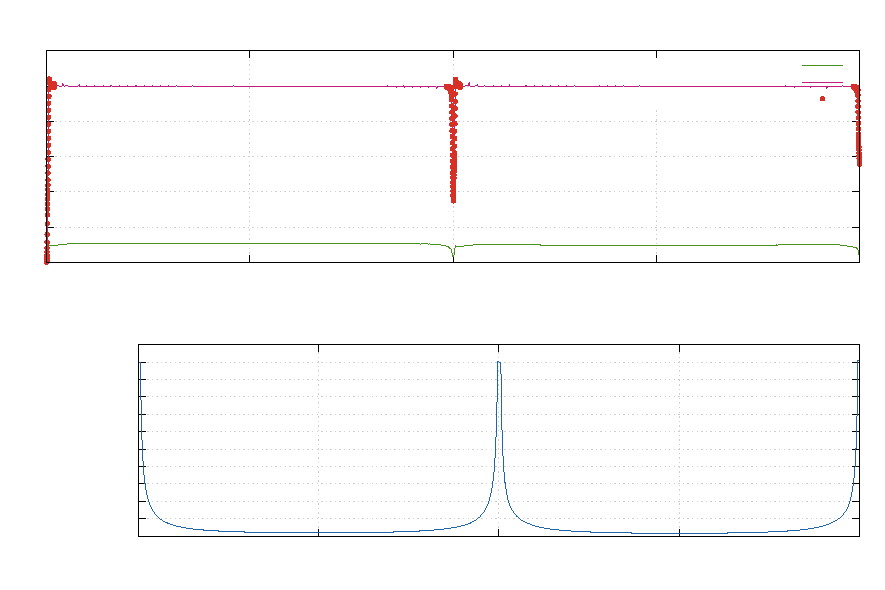
\includegraphics[width={425.00bp},height={283.00bp}]{assignment6_convergence}}%
    \gplfronttext
  \end{picture}%
\endgroup
}
  \caption{Adaptive timestep behaviour over the postoperative proof-of-concept
  cycle. Red markers denote sampled timesteps that reached three PIMPLE outer
  correctors without meeting the selected outer criterion. These events cluster
  around zero-flow transitions rather than peak-flow intervals.}
  \label{fig:transient_residuals}
\end{figure}

\subsection{Velocity vectors at representative phases}

Three saved states were selected directly from the waveform:
$t=\SI{0.24}{\second}$ represents accelerating inspiration at approximately
68.5\% of peak flow, $t=\SI{0.50}{\second}$ is peak inspiration, and
$t=\SI{1.50}{\second}$ is peak expiration. The two peak states isolate reversal
of the velocity field at equal flow magnitude, while the accelerating state
shows development of the inspiratory jet.

\begin{figure}[htbp]
  \centering
  \begin{subfigure}[t]{0.48\textwidth}
    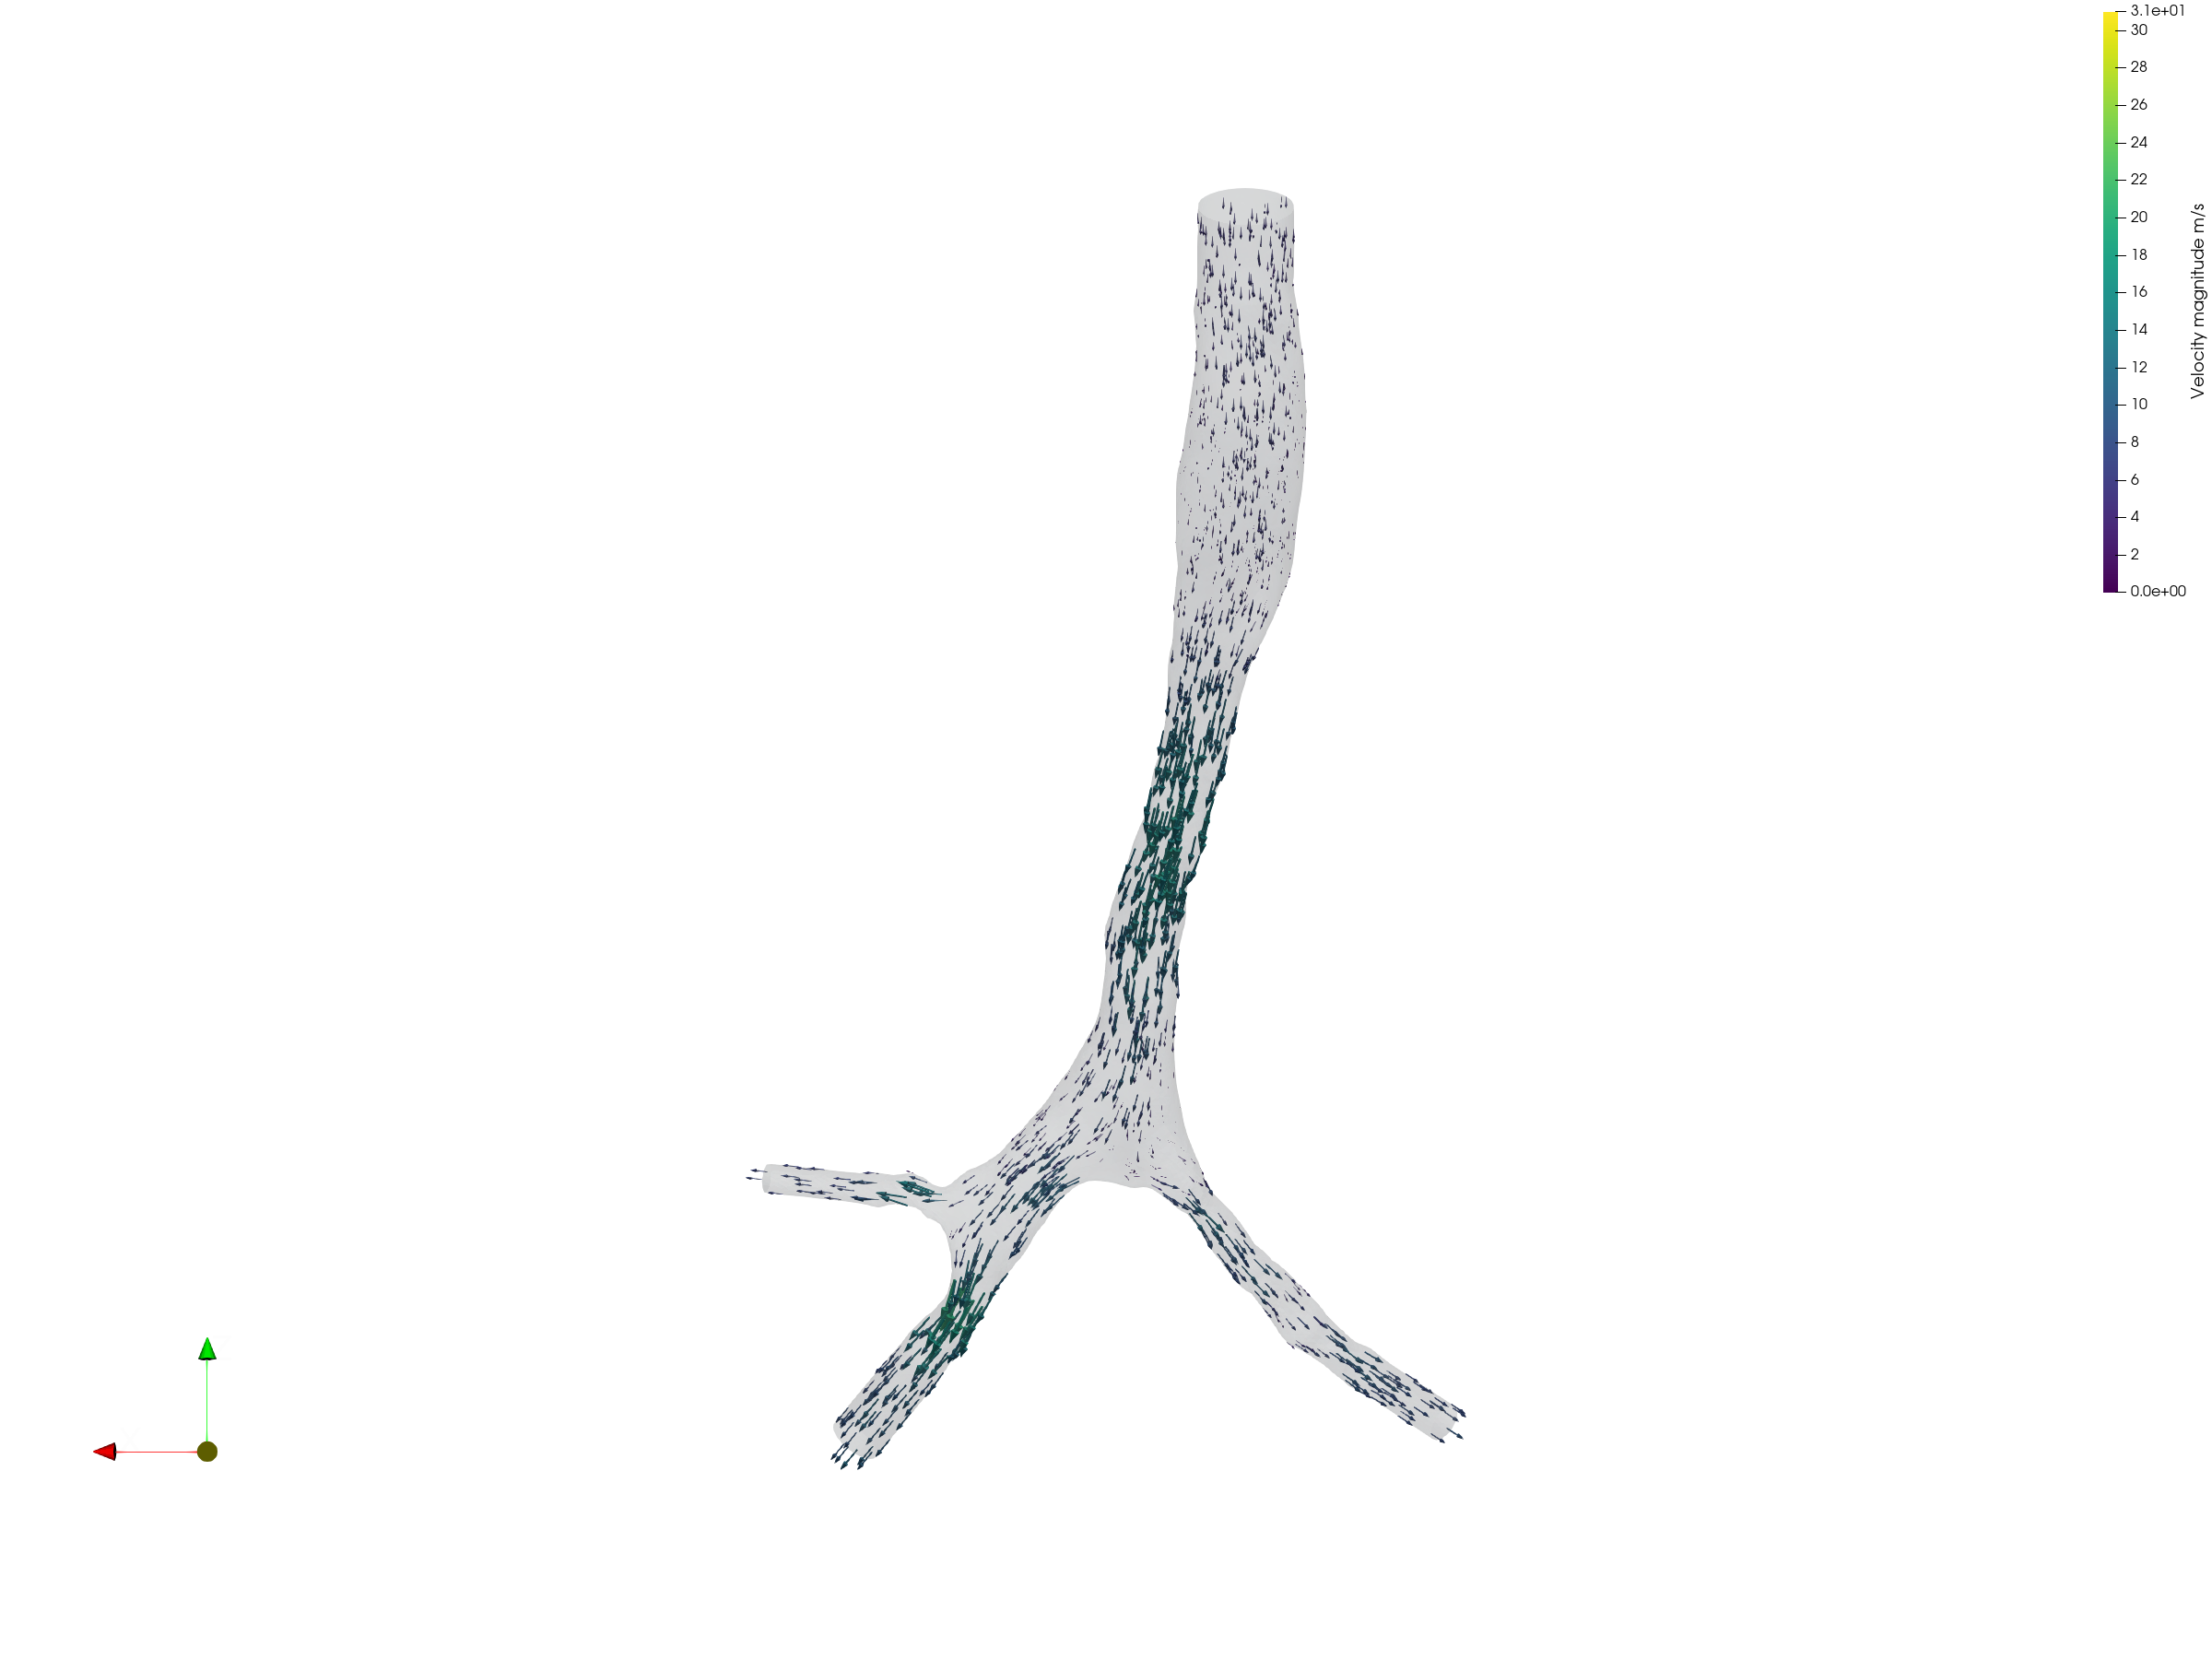
\includegraphics[width=\linewidth]{assignment6_vectors_024.png}
    \caption{$t=\SI{0.24}{\second}$; $Q=\SI{4.30}{\litre\per\minute}$.}
  \end{subfigure}\hfill
  \begin{subfigure}[t]{0.48\textwidth}
    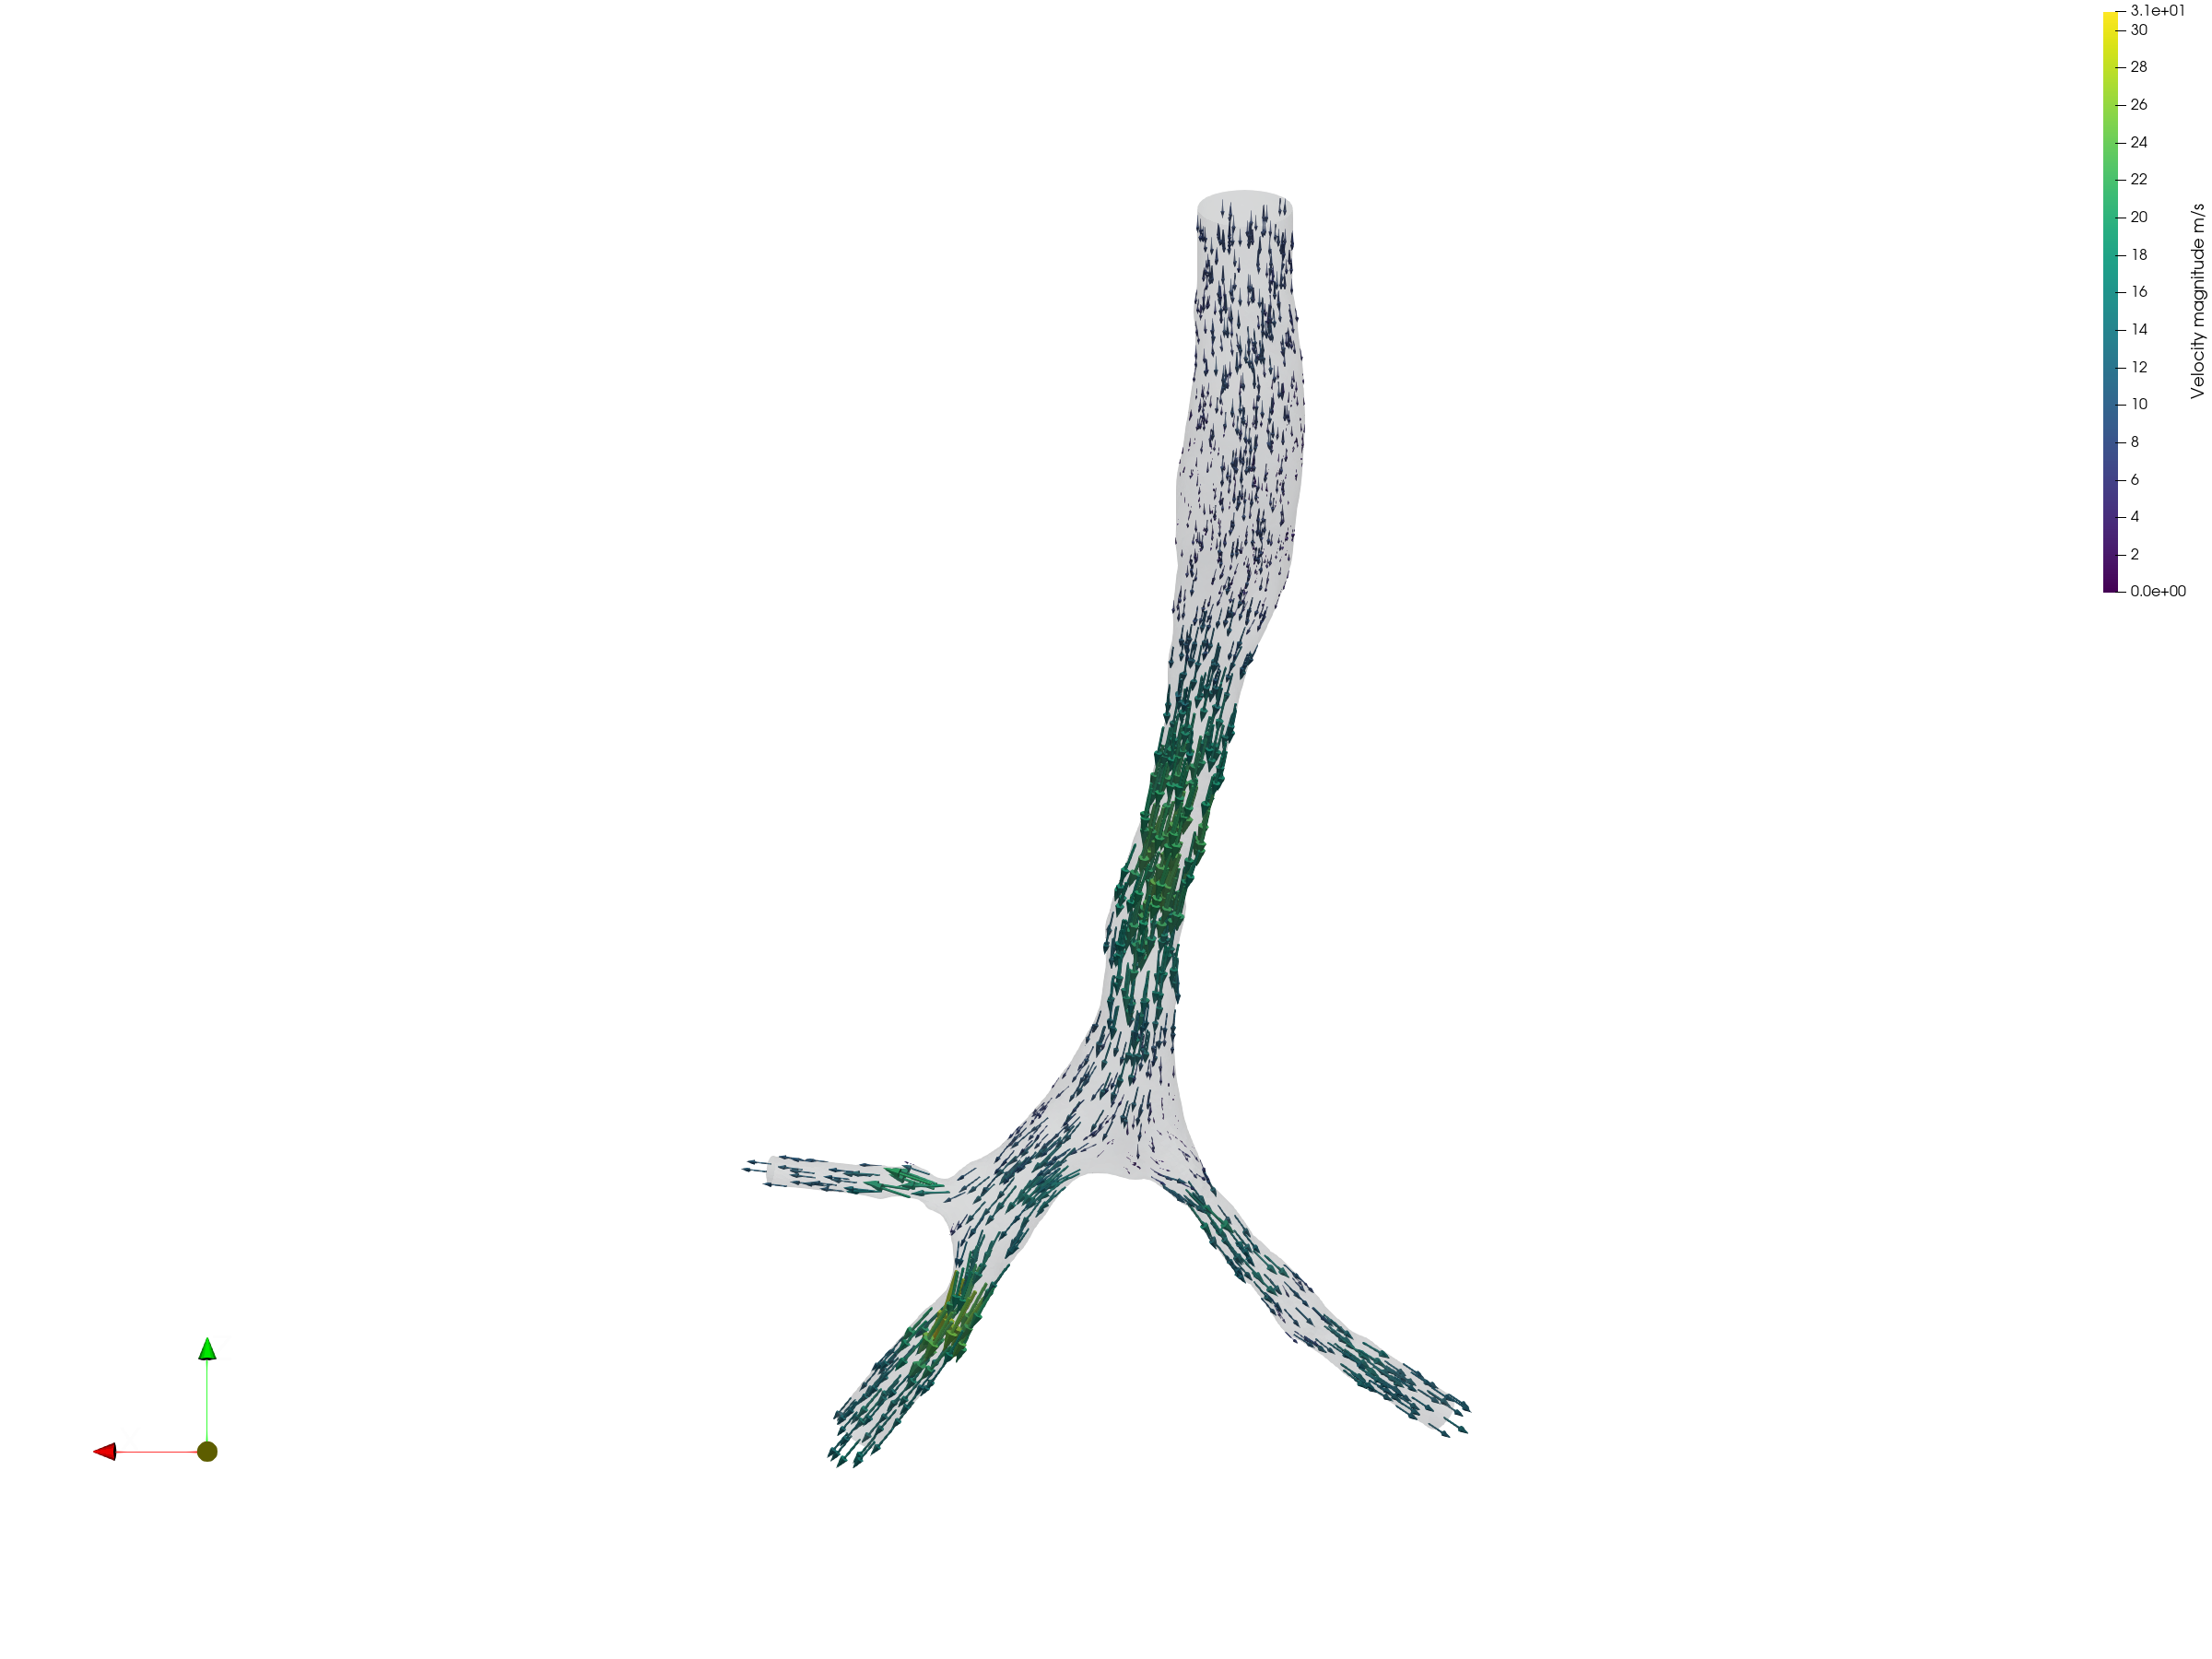
\includegraphics[width=\linewidth]{assignment6_vectors_050.png}
    \caption{$t=\SI{0.50}{\second}$; $Q=\SI{6.29}{\litre\per\minute}$.}
  \end{subfigure}

  \medskip
  \begin{subfigure}[t]{0.48\textwidth}
    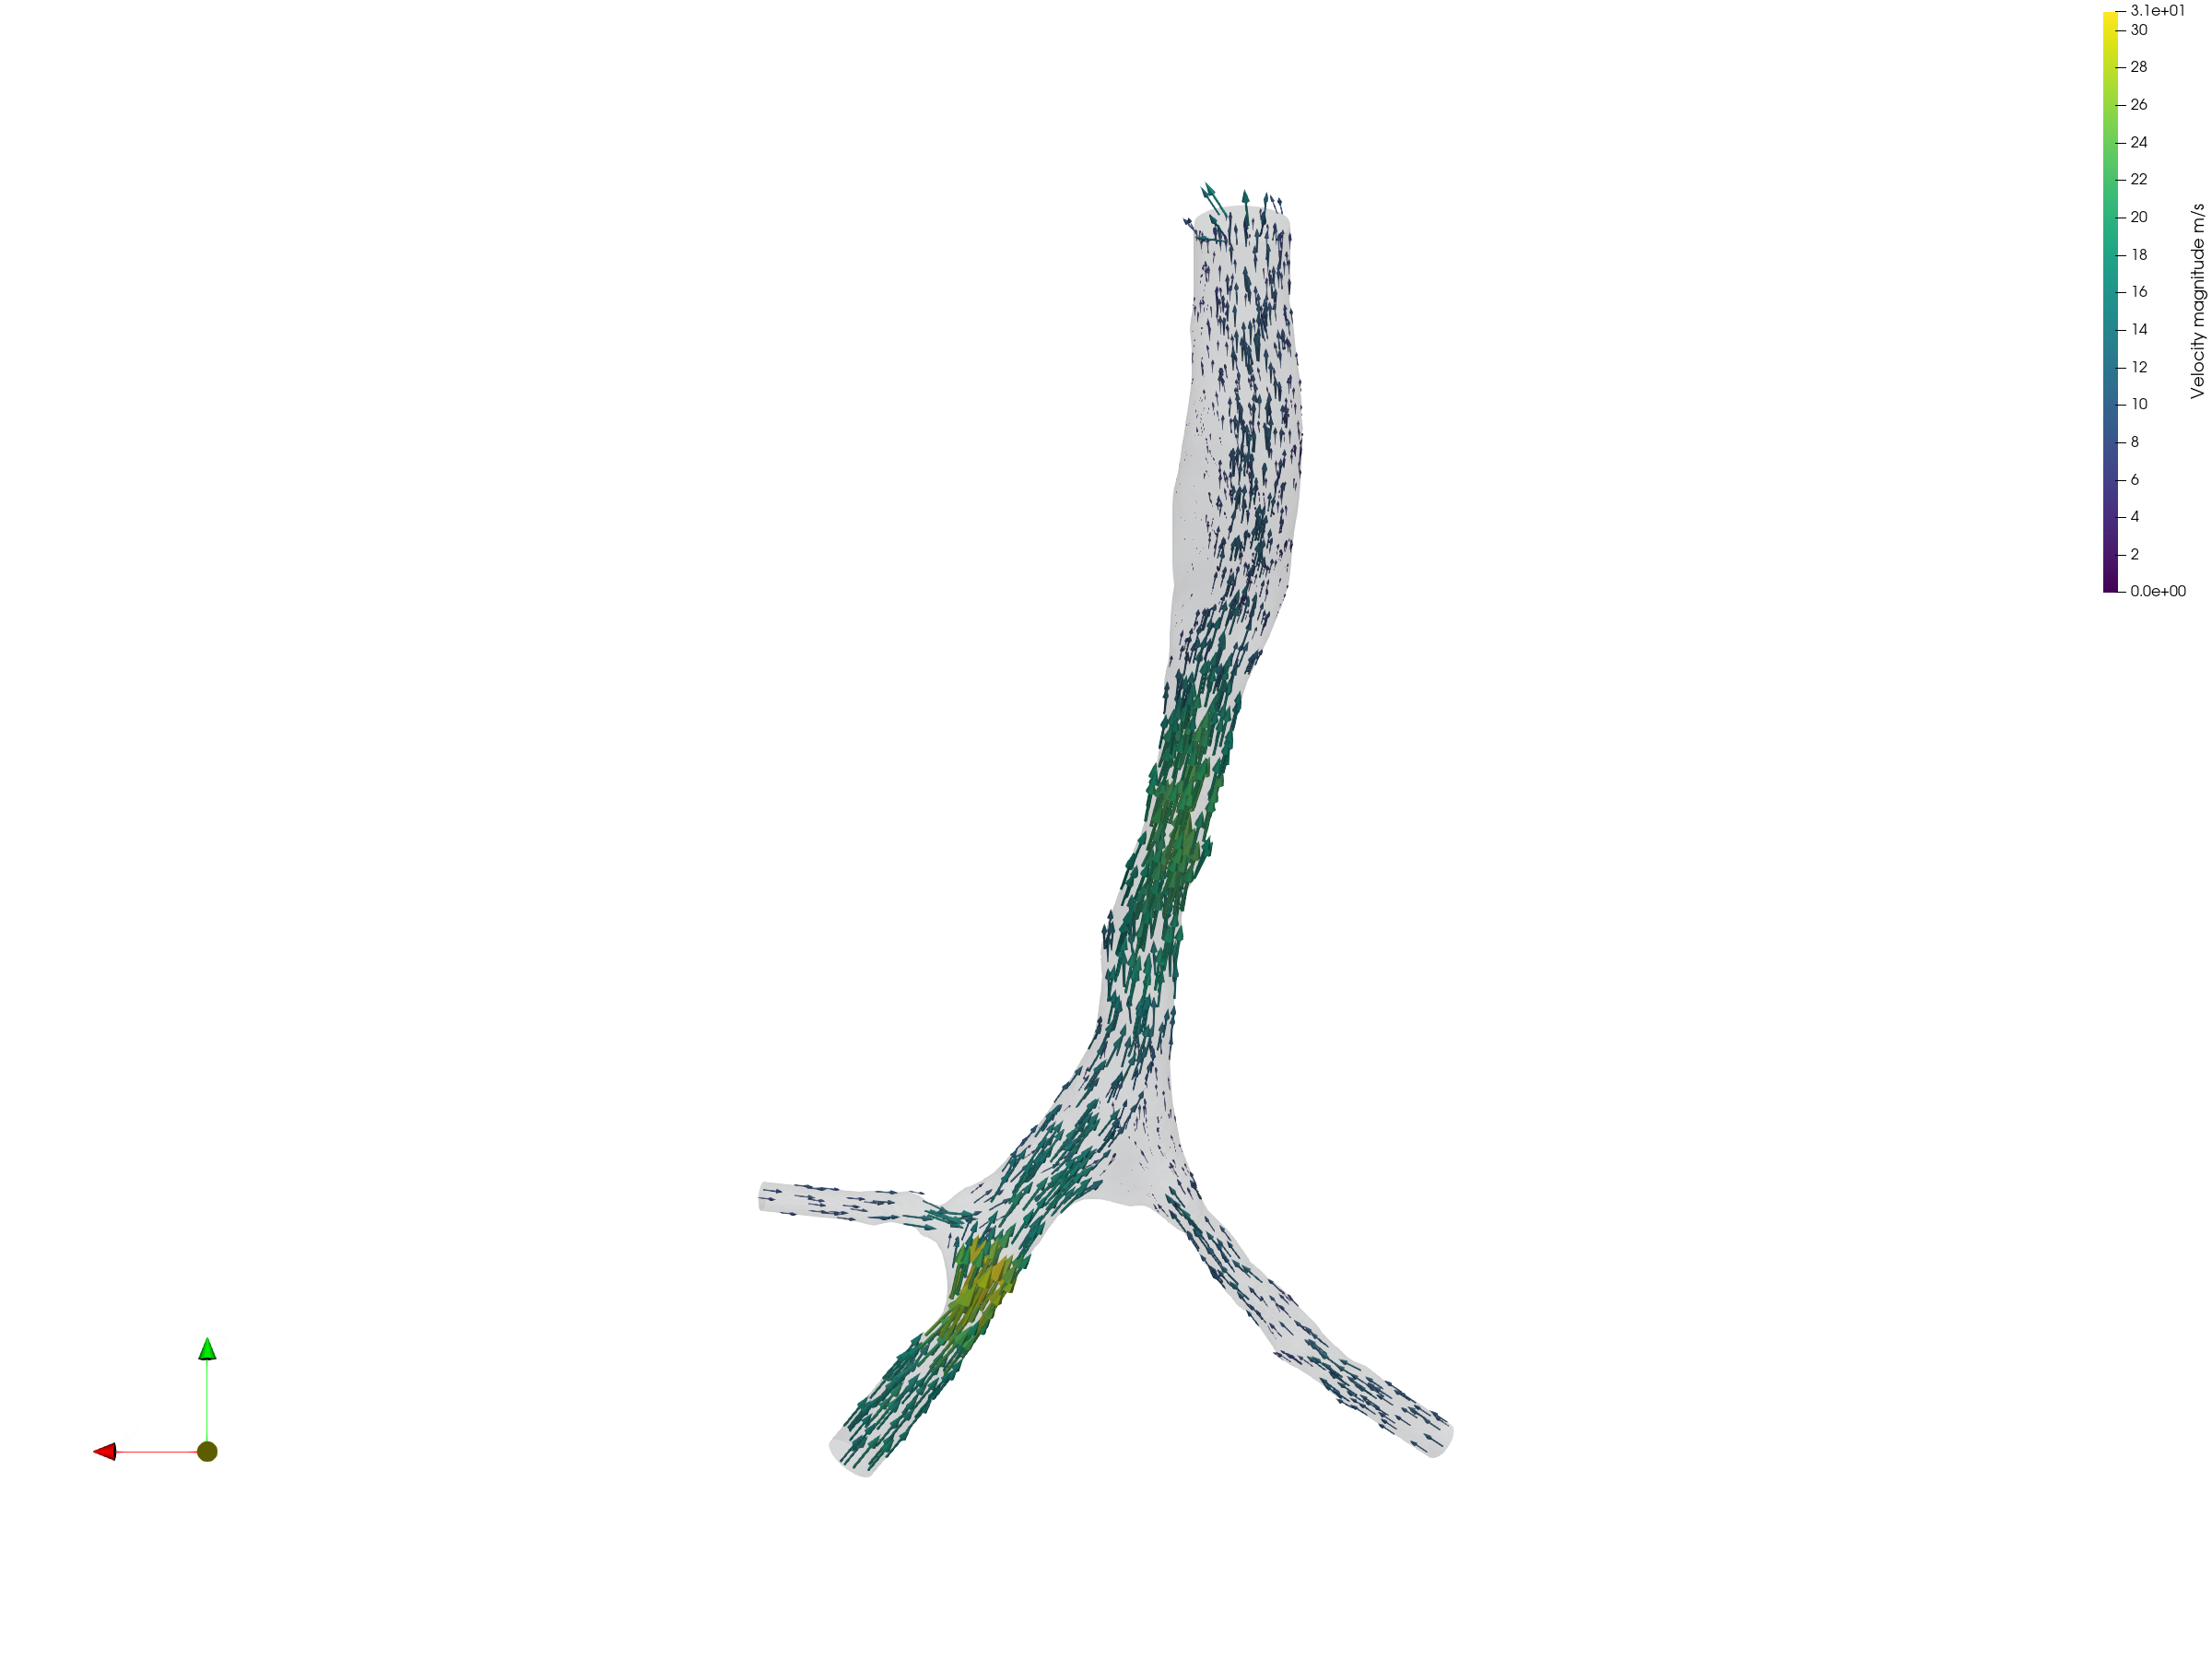
\includegraphics[width=\linewidth]{assignment6_vectors_150.png}
    \caption{$t=\SI{1.50}{\second}$; $Q=\SI{-6.29}{\litre\per\minute}$.}
  \end{subfigure}
  \caption{Postoperative transient velocity vectors using one anatomical frontal
  view and a common \SIrange{0}{31}{\metre\per\second} scale. The third panel
  demonstrates reversal during expiration.}
  \label{fig:transient_vectors}
\end{figure}

\subsection{Breathing waveform and time-varying resistance}

The applied section flow and local pressure difference were evaluated on the
same planes as Assignment 4 at all 100 nonzero saved times. Flow ranged from
\SI{-6.288}{\litre\per\minute} to \SI{6.288}{\litre\per\minute}, and pressure
drop ranged from \SI{-58.70}{\pascal} to \SI{167.45}{\pascal}. Resistance was
masked where $|Q|$ was below 5\% of peak flow because division by a near-zero
flow is ill-conditioned. Over the retained states it ranged from
\SI{5.71}{\pascal\per\litre\per\minute} to
\SI{26.63}{\pascal\per\litre\per\minute}. Unlike ideal constant Poiseuille
resistance, the patient-specific result depends on flow direction and phase due
to developing flow, curvature, branching, separation, and unsteady inertia.
The preoperative airway was not simulated transiently; its 64.9\% area
constriction supports only a qualitative expectation of higher resistance.

\begin{figure}[htbp]
  \centering
  \resizebox{0.92\textwidth}{!}{% GNUPLOT: LaTeX picture with Postscript
\begingroup
  \makeatletter
  \providecommand\color[2][]{%
    \GenericError{(gnuplot) \space\space\space\@spaces}{%
      Package color not loaded in conjunction with
      terminal option `colourtext'%
    }{See the gnuplot documentation for explanation.%
    }{Either use 'blacktext' in gnuplot or load the package
      color.sty in LaTeX.}%
    \renewcommand\color[2][]{}%
  }%
  \providecommand\includegraphics[2][]{%
    \GenericError{(gnuplot) \space\space\space\@spaces}{%
      Package graphicx or graphics not loaded%
    }{See the gnuplot documentation for explanation.%
    }{The gnuplot epslatex terminal needs graphicx.sty or graphics.sty.}%
    \renewcommand\includegraphics[2][]{}%
  }%
  \providecommand\rotatebox[2]{#2}%
  \@ifundefined{ifGPcolor}{%
    \newif\ifGPcolor
    \GPcolortrue
  }{}%
  \@ifundefined{ifGPblacktext}{%
    \newif\ifGPblacktext
    \GPblacktexttrue
  }{}%
  % define a \g@addto@macro without @ in the name:
  \let\gplgaddtomacro\g@addto@macro
  % define empty templates for all commands taking text:
  \gdef\gplbacktext{}%
  \gdef\gplfronttext{}%
  \makeatother
  \ifGPblacktext
    % no textcolor at all
    \def\colorrgb#1{}%
    \def\colorgray#1{}%
  \else
    % gray or color?
    \ifGPcolor
      \def\colorrgb#1{\color[rgb]{#1}}%
      \def\colorgray#1{\color[gray]{#1}}%
      \expandafter\def\csname LTw\endcsname{\color{white}}%
      \expandafter\def\csname LTb\endcsname{\color{black}}%
      \expandafter\def\csname LTa\endcsname{\color{black}}%
      \expandafter\def\csname LT0\endcsname{\color[rgb]{1,0,0}}%
      \expandafter\def\csname LT1\endcsname{\color[rgb]{0,1,0}}%
      \expandafter\def\csname LT2\endcsname{\color[rgb]{0,0,1}}%
      \expandafter\def\csname LT3\endcsname{\color[rgb]{1,0,1}}%
      \expandafter\def\csname LT4\endcsname{\color[rgb]{0,1,1}}%
      \expandafter\def\csname LT5\endcsname{\color[rgb]{1,1,0}}%
      \expandafter\def\csname LT6\endcsname{\color[rgb]{0,0,0}}%
      \expandafter\def\csname LT7\endcsname{\color[rgb]{1,0.3,0}}%
      \expandafter\def\csname LT8\endcsname{\color[rgb]{0.5,0.5,0.5}}%
    \else
      % gray
      \def\colorrgb#1{\color{black}}%
      \def\colorgray#1{\color[gray]{#1}}%
      \expandafter\def\csname LTw\endcsname{\color{white}}%
      \expandafter\def\csname LTb\endcsname{\color{black}}%
      \expandafter\def\csname LTa\endcsname{\color{black}}%
      \expandafter\def\csname LT0\endcsname{\color{black}}%
      \expandafter\def\csname LT1\endcsname{\color{black}}%
      \expandafter\def\csname LT2\endcsname{\color{black}}%
      \expandafter\def\csname LT3\endcsname{\color{black}}%
      \expandafter\def\csname LT4\endcsname{\color{black}}%
      \expandafter\def\csname LT5\endcsname{\color{black}}%
      \expandafter\def\csname LT6\endcsname{\color{black}}%
      \expandafter\def\csname LT7\endcsname{\color{black}}%
      \expandafter\def\csname LT8\endcsname{\color{black}}%
    \fi
  \fi
    \setlength{\unitlength}{0.0500bp}%
    \ifx\gptboxheight\undefined%
      \newlength{\gptboxheight}%
      \newlength{\gptboxwidth}%
      \newsavebox{\gptboxtext}%
    \fi%
    \setlength{\fboxrule}{0.5pt}%
    \setlength{\fboxsep}{1pt}%
    \definecolor{tbcol}{rgb}{1,1,1}%
\begin{picture}(8500.00,6220.00)%
    \gplgaddtomacro\gplbacktext{%
      \csname LTb\endcsname%%
      \put(438,3416){\makebox(0,0)[r]{\strut{}$-8$}}%
      \csname LTb\endcsname%%
      \put(438,3705){\makebox(0,0)[r]{\strut{}$-6$}}%
      \csname LTb\endcsname%%
      \put(438,3993){\makebox(0,0)[r]{\strut{}$-4$}}%
      \csname LTb\endcsname%%
      \put(438,4282){\makebox(0,0)[r]{\strut{}$-2$}}%
      \csname LTb\endcsname%%
      \put(438,4570){\makebox(0,0)[r]{\strut{}$0$}}%
      \csname LTb\endcsname%%
      \put(438,4859){\makebox(0,0)[r]{\strut{}$2$}}%
      \csname LTb\endcsname%%
      \put(438,5147){\makebox(0,0)[r]{\strut{}$4$}}%
      \csname LTb\endcsname%%
      \put(438,5436){\makebox(0,0)[r]{\strut{}$6$}}%
      \csname LTb\endcsname%%
      \put(438,5724){\makebox(0,0)[r]{\strut{}$8$}}%
      \csname LTb\endcsname%%
      \put(518,3258){\makebox(0,0){\strut{}$0$}}%
      \csname LTb\endcsname%%
      \put(1389,3258){\makebox(0,0){\strut{}$0.5$}}%
      \csname LTb\endcsname%%
      \put(2259,3258){\makebox(0,0){\strut{}$1$}}%
      \csname LTb\endcsname%%
      \put(3129,3258){\makebox(0,0){\strut{}$1.5$}}%
      \csname LTb\endcsname%%
      \put(3999,3258){\makebox(0,0){\strut{}$2$}}%
    }%
    \gplgaddtomacro\gplfronttext{%
      \csname LTb\endcsname%%
      \put(3375,5582){\makebox(0,0)[r]{\strut{}Section flow}}%
      \csname LTb\endcsname%%
      \put(139,4570){\rotatebox{-270.00}{\makebox(0,0){\strut{}Flow rate (L/min)}}}%
      \csname LTb\endcsname%%
      \put(2259,5962){\makebox(0,0){\strut{}Postoperative breathing-cycle response}}%
    }%
    \gplgaddtomacro\gplbacktext{%
      \csname LTb\endcsname%%
      \put(4838,3416){\makebox(0,0)[r]{\strut{}$-100$}}%
      \csname LTb\endcsname%%
      \put(4838,3801){\makebox(0,0)[r]{\strut{}$-50$}}%
      \csname LTb\endcsname%%
      \put(4838,4186){\makebox(0,0)[r]{\strut{}$0$}}%
      \csname LTb\endcsname%%
      \put(4838,4570){\makebox(0,0)[r]{\strut{}$50$}}%
      \csname LTb\endcsname%%
      \put(4838,4955){\makebox(0,0)[r]{\strut{}$100$}}%
      \csname LTb\endcsname%%
      \put(4838,5340){\makebox(0,0)[r]{\strut{}$150$}}%
      \csname LTb\endcsname%%
      \put(4838,5724){\makebox(0,0)[r]{\strut{}$200$}}%
      \csname LTb\endcsname%%
      \put(4919,3258){\makebox(0,0){\strut{}$0$}}%
      \csname LTb\endcsname%%
      \put(5749,3258){\makebox(0,0){\strut{}$0.5$}}%
      \csname LTb\endcsname%%
      \put(6579,3258){\makebox(0,0){\strut{}$1$}}%
      \csname LTb\endcsname%%
      \put(7409,3258){\makebox(0,0){\strut{}$1.5$}}%
      \csname LTb\endcsname%%
      \put(8239,3258){\makebox(0,0){\strut{}$2$}}%
    }%
    \gplgaddtomacro\gplfronttext{%
      \csname LTb\endcsname%%
      \put(4379,4570){\rotatebox{-270.00}{\makebox(0,0){\strut{}$Delta P$ (Pa)}}}%
      \csname LTb\endcsname%%
      \put(6579,5962){\makebox(0,0){\strut{}Postoperative breathing-cycle response}}%
    }%
    \gplgaddtomacro\gplbacktext{%
      \csname LTb\endcsname%%
      \put(438,506){\makebox(0,0)[r]{\strut{}$0$}}%
      \csname LTb\endcsname%%
      \put(438,859){\makebox(0,0)[r]{\strut{}$5$}}%
      \csname LTb\endcsname%%
      \put(438,1212){\makebox(0,0)[r]{\strut{}$10$}}%
      \csname LTb\endcsname%%
      \put(438,1565){\makebox(0,0)[r]{\strut{}$15$}}%
      \csname LTb\endcsname%%
      \put(438,1918){\makebox(0,0)[r]{\strut{}$20$}}%
      \csname LTb\endcsname%%
      \put(438,2271){\makebox(0,0)[r]{\strut{}$25$}}%
      \csname LTb\endcsname%%
      \put(438,2624){\makebox(0,0)[r]{\strut{}$30$}}%
      \csname LTb\endcsname%%
      \put(518,348){\makebox(0,0){\strut{}$0$}}%
      \csname LTb\endcsname%%
      \put(1389,348){\makebox(0,0){\strut{}$0.5$}}%
      \csname LTb\endcsname%%
      \put(2259,348){\makebox(0,0){\strut{}$1$}}%
      \csname LTb\endcsname%%
      \put(3129,348){\makebox(0,0){\strut{}$1.5$}}%
      \csname LTb\endcsname%%
      \put(3999,348){\makebox(0,0){\strut{}$2$}}%
    }%
    \gplgaddtomacro\gplfronttext{%
      \csname LTb\endcsname%%
      \put(139,1565){\rotatebox{-270.00}{\makebox(0,0){\strut{}$R$ (Pa/(L/min))}}}%
      \csname LTb\endcsname%%
      \put(2259,110){\makebox(0,0){\strut{}Time (s)}}%
      \csname LTb\endcsname%%
      \put(2259,2862){\makebox(0,0){\strut{}Postoperative breathing-cycle response}}%
    }%
    \gplgaddtomacro\gplbacktext{%
      \csname LTb\endcsname%%
      \put(4758,506){\makebox(0,0)[r]{\strut{}$0$}}%
      \csname LTb\endcsname%%
      \put(4758,809){\makebox(0,0)[r]{\strut{}$0.5$}}%
      \csname LTb\endcsname%%
      \put(4758,1111){\makebox(0,0)[r]{\strut{}$1$}}%
      \csname LTb\endcsname%%
      \put(4758,1414){\makebox(0,0)[r]{\strut{}$1.5$}}%
      \csname LTb\endcsname%%
      \put(4758,1717){\makebox(0,0)[r]{\strut{}$2$}}%
      \csname LTb\endcsname%%
      \put(4758,2019){\makebox(0,0)[r]{\strut{}$2.5$}}%
      \csname LTb\endcsname%%
      \put(4758,2322){\makebox(0,0)[r]{\strut{}$3$}}%
      \csname LTb\endcsname%%
      \put(4758,2624){\makebox(0,0)[r]{\strut{}$3.5$}}%
      \csname LTb\endcsname%%
      \put(4838,348){\makebox(0,0){\strut{}$0$}}%
      \csname LTb\endcsname%%
      \put(5689,348){\makebox(0,0){\strut{}$0.5$}}%
      \csname LTb\endcsname%%
      \put(6539,348){\makebox(0,0){\strut{}$1$}}%
      \csname LTb\endcsname%%
      \put(7389,348){\makebox(0,0){\strut{}$1.5$}}%
      \csname LTb\endcsname%%
      \put(8239,348){\makebox(0,0){\strut{}$2$}}%
    }%
    \gplgaddtomacro\gplfronttext{%
      \csname LTb\endcsname%%
      \put(4379,1565){\rotatebox{-270.00}{\makebox(0,0){\strut{}Qualitative resistance (a.u.)}}}%
      \csname LTb\endcsname%%
      \put(6539,110){\makebox(0,0){\strut{}Time (s)}}%
      \csname LTb\endcsname%%
      \put(6539,2862){\makebox(0,0){\strut{}Conceptual anatomical comparison (not CFD)}}%
    }%
    \gplbacktext
    \put(0,0){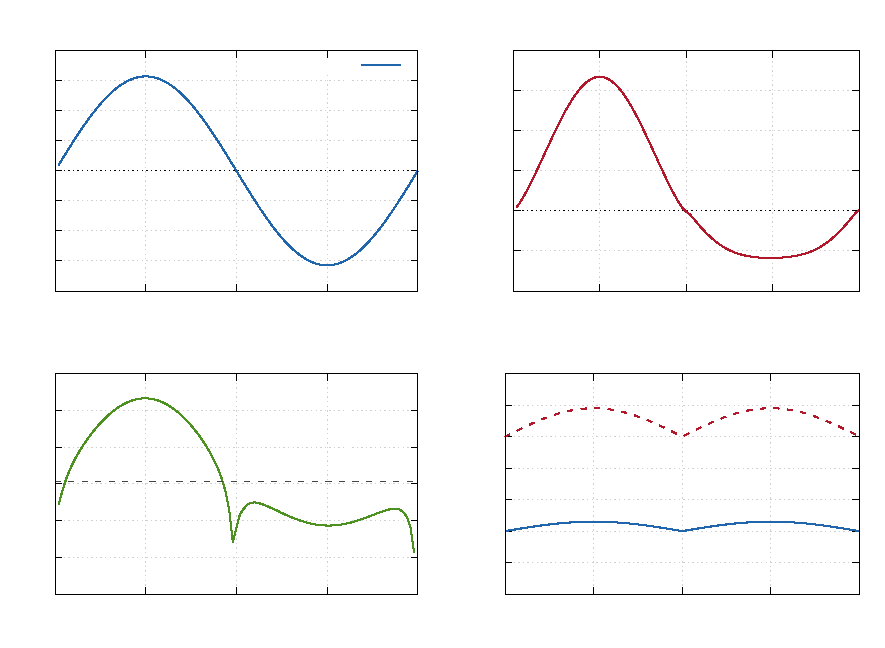
\includegraphics[width={425.00bp},height={311.00bp}]{assignment6_cycle_response}}%
    \gplfronttext
  \end{picture}%
\endgroup
}
  \caption{Complete-cycle section flow, local pressure difference, and
  postoperative local resistance. Resistance is omitted when
  $|Q|<\SI{0.314}{\litre\per\minute}$ (5\% of peak flow). The dashed line is the
  steady coarse-mesh resistance at \SI{2}{\litre\per\minute}; it is a reference,
  not an expected constant for this patient-specific unsteady flow. The
  arbitrary-unit comparison is explicitly conceptual: only the postoperative
  cycle was simulated transiently.}
  \label{fig:transient_resistance}
\end{figure}

% -----------------------------------------------------------------------------
\section{Discussion}
\label{sec:discussion}

\subsection{Interpretation of outlet conditions and lung-flow split}

Applying the same static pressure at every distal outlet deliberately leaves the
left/right flow division unconstrained, making it an output of the reconstructed
geometry rather than an imposed boundary-condition ratio. The predicted
73.17\% right and 26.83\% left distribution is therefore a defensible measure of
the relative aerodynamic resistance of the resolved postoperative branches.
Differences in calibre, pathway length, branching angle, curvature, and local
flow separation can all contribute to the unequal result.

This distribution should not, however, be interpreted as the child's measured
physiological lung ventilation. The model ends at truncated bronchial outlets and
therefore excludes the resistance of unresolved peripheral airways and the
compliance of the distal lungs. A more physiologically detailed extension could
apply distal resistance conditions such as

\begin{equation}
  P_i = P_{\mathrm{alv}} + R_i Q_i,
\end{equation}

or coupled resistance--compliance outlet models. Such conditions would preserve
an emergent flow split while representing peripheral lung mechanics, provided
that patient-specific parameters were available.

\subsection{Mesh sensitivity and optimal mesh}

Resistance and the small right-superior branch split were more mesh-sensitive
than total right-lung fraction. From 0.15 to 0.12 mm, all selected metrics changed
by at most 2.02\%, while cell count increased by 92\% and solver execution time
by 157\%. The 0.12 mm case also failed residual control at 2000 iterations,
whereas 0.15 mm converged in 1611. With a practical 2.5\% acceptance threshold,
the 0.15 mm mesh is selected as the optimal balance between apparent spatial
convergence and computational efficiency.

\subsection{Constant-diameter resistance during inspiration}

For fully developed laminar flow in a rigid constant-diameter tube,
Poiseuille's law gives $\Delta P=128\mu LQ/(\pi D^4)=RQ$. The viscous pressure
loss therefore increases linearly with flow, but $R=\Delta P/Q$ remains constant.
Thus, it would be imprecise to attribute the observed increase in effective
resistance to linear viscous friction alone.

A useful reduced description of the patient-specific transient pressure loss is

\begin{equation}
  \Delta P(t)=aQ(t)+b|Q(t)|Q(t)+L_f\frac{\mathrm{d}Q}{\mathrm{d}t},
  \label{eq:nonlinear_pressure_loss}
\end{equation}

where $aQ$ represents approximately linear viscous loss, $b|Q|Q$ represents
flow-dependent convective and form losses, and $L_f\,\mathrm{d}Q/\mathrm{d}t$
represents fluid inertance. Dividing by $Q$ away from flow reversal gives an
apparent resistance containing $a+b|Q|$ and an acceleration-dependent term.
Consequently, effective resistance can rise with inspiratory flow as jets,
developing profiles, curvature, branching, and separation increase dissipation.
This is consistent with the computed inspiratory increase from approximately
\SI{12.3}{\pascal\per\litre\per\minute} at \SI{0.40}{\litre\per\minute} to
\SI{26.6}{\pascal\per\litre\per\minute} near peak inspiration. The lower and
asymmetric expiratory branch is physically possible for reversed flow through a
non-symmetric geometry, but its magnitude remains sensitive to inertia, outlet
conditions, the initial cycle, and the coarse high-Courant discretisation.

\subsection{Limitations}

Potential limitations include:

\begin{itemize}
  \item static CT geometry despite the dynamic nature of tracheomalacia;
  \item rigid airway walls and absence of fluid--structure interaction;
  \item an idealised sinusoidal waveform rather than a measured patient-specific waveform;
  \item idealised outlet pressure conditions;
  \item uncertainty from segmentation and clipping-point placement;
  \item an isotropic first-order tetrahedral mesh without dedicated prism
        boundary layers;
  \item the selected laminar-flow assumption; and
  \item analysis of a limited number of anatomical cases.
\end{itemize}

With additional resources, refinement should focus locally on the matched
tracheal region, carina, and small right-superior branch rather than reducing
global size uniformly. All cases should first meet residual and monitored-integral
criteria. Additional levels around the apparent asymptotic range, consistently
generated prism layers, Richardson extrapolation, and a grid-convergence index
would strengthen numerical uncertainty estimates. Runtime, memory, mesh quality,
and section-area variation should be tracked alongside each physical metric.

\subsection{Handling transient non-convergence}

The 617 outer-criterion failures were concentrated around startup and the two
zero-flow transitions, where pressure and velocity fields must adjust while the
flow changes direction. The first remedy would be to repeat those intervals with
a lower Courant limit, because this directly improves temporal resolution and
pressure--velocity coupling. If failures persisted, the number of outer or
pressure correctors would be increased. A converged previous cycle would provide
a better initial condition than rest, and additional cycles would be simulated
until corresponding phase metrics became periodic. Finally, the cells identified
by the three failed \texttt{checkMesh} checks should be repaired before a
quantitative production run. These changes target the observed causes without
misrepresenting the present proof-of-concept result.

% -----------------------------------------------------------------------------
\section{Conclusions}
\label{sec:conclusions}

The preoperative minimum lumen area was \SI{1.813}{\milli\metre\squared},
compared with \SI{5.169}{\milli\metre\squared} at the corresponding
postoperative location, giving a 64.9\% area constriction and demonstrating a
substantial anatomical increase after intervention. Steady postoperative CFD at
\SI{2}{\litre\per\minute} predicted a local pressure drop of
\SI{30.95}{\pascal}, resistance of
\SI{15.41}{\pascal\per\litre\per\minute}, peak velocity of
\SI{9.25}{\metre\per\second}, and a geometry-driven 73.17/26.83\% right/left
flow split. The \num{0.15}~mm HXT mesh was selected for steady analysis because
its monitored metrics differed from the densest mesh by at most 2.02\% while
avoiding its convergence and cost penalty.

A complete postoperative transient proof of concept produced the prescribed
$\pm\SI{6.283}{\litre\per\minute}$ cycle and direction-dependent resistance
between \SI{5.71}{\pascal\per\litre\per\minute} and
\SI{26.63}{\pascal\per\litre\per\minute} outside masked zero-flow intervals.
Although 99.826\% of timesteps met the PIMPLE criterion, the coarse mesh,
$\mathrm{Co}_{\max}=5$, failed mesh-quality checks, and absence of timestep
independence limit this result to qualitative phase trends. The anatomical and
steady integral conclusions are therefore stronger than the transient extrema.

% -----------------------------------------------------------------------------
\section*{Reproducibility statement}
\addcontentsline{toc}{section}{Reproducibility statement}

The complete workflow is documented in \texttt{WORKFLOW.md}. Record the Git
commit, Slicer version, Gmsh version, OpenFOAM image identifier, mesh sizes,
cell counts, and solver settings used for the final results. The scripts
\texttt{create\_volume\_mesh.sh}, \texttt{run\_cfd.sh},
\texttt{run\_fine\_cfd.sh}, and \texttt{fetch\_cfd\_results.sh} automate the
meshing, remote execution, reconstruction, and retrieval stages.

% -----------------------------------------------------------------------------
% Appendices
% -----------------------------------------------------------------------------
\clearpage
\appendix

\section{OpenFOAM}
\label{app:openfoam}

OpenFOAM is an open-source computational continuum-mechanics framework that
uses the finite-volume method. Conservation equations are integrated over each
mesh cell and the divergence theorem converts volume derivatives into fluxes
through its faces. Interpolation and gradient schemes provide face values from
cell-centred quantities, producing sparse algebraic systems for velocity
$\mathbf{U}$ and pressure $p$ \cite{openfoam}. OpenFOAM uses kinematic pressure
for incompressible flow,

\begin{equation}
  p=\frac{P}{\rho},
\end{equation}

with units of \si{\metre\squared\per\second\squared}; dimensional pressure
differences in this report are therefore recovered from
$\Delta P=\rho\,\Delta p$. For incompressible Newtonian laminar flow, the
solvers considered here discretise

\begin{align}
  \nabla\cdot\mathbf{U} &= 0, \\
  \frac{\partial\mathbf{U}}{\partial t}
  +\nabla\cdot(\mathbf{U}\mathbf{U})
  &= -\nabla p
     +\nabla\cdot\left[\nu\left(\nabla\mathbf{U}
     +\nabla\mathbf{U}^{T}\right)\right].
\end{align}

The transient term is omitted in a steady calculation. Pressure and velocity
are coupled physically but solved in a segregated manner. A discretised
momentum equation may be written schematically as

\begin{equation}
  A_U\mathbf{U}=\mathbf{H}(\mathbf{U})-\nabla p.
\end{equation}

Using the reciprocal diagonal coefficient $r_{AU}=1/A_U$ gives a predicted
velocity and face flux. Requiring the corrected flux to be divergence-free
then produces a pressure equation of the form

\begin{equation}
  \nabla\cdot\left(r_{AU}\nabla p\right)
  =\nabla\cdot\boldsymbol{\phi}_{H/A}.
\end{equation}

The resulting pressure correction updates both velocity and face flux, thereby
progressively enforcing mass conservation. On a non-orthogonal mesh, pressure
correction is repeated so that explicitly treated non-orthogonal contributions
are updated before the final conservative flux correction.

\subsection{The \texttt{simpleFoam} solver}

\texttt{simpleFoam} is a steady-state incompressible solver. It uses the SIMPLE
algorithm: (1) assemble and solve the momentum equations using the current
pressure; (2) construct and solve a pressure-correction equation; (3) correct
pressure, velocity, and face flux; (4) update boundary conditions; and (5)
repeat until convergence. Its iterations are numerical fixed-point iterations
and do not represent physical time. Under-relaxation limits field changes
between iterations and can stabilise pressure--velocity coupling.

In this study, pressure is solved using GAMG and velocity with
\texttt{smoothSolver} using symmetric Gauss--Seidel smoothing. Two
non-orthogonal correctors are applied in the steady case. The SIMPLE residual
controls are $10^{-5}$ for pressure and $10^{-6}$ for velocity. The Assignment
4 postoperative solution met these criteria after 589 iterations. Convergence
is additionally assessed through integrated inlet/outlet flow because small
algebraic residuals alone do not guarantee conservation of the reported
quantity.

\subsection{The \texttt{pimpleFoam} solver}

\texttt{pimpleFoam} advances the incompressible equations through physical time
using PIMPLE, which combines SIMPLE-like outer iterations with PISO-like inner
pressure correctors. At each new time level, time-dependent boundary conditions
are updated and a momentum equation is assembled. Each outer corrector updates
the nonlinear momentum terms; within it, pressure correctors repeatedly enforce
continuity and update $p$, $\mathbf{U}$, and the face flux. More correctors can
improve coupling at a timestep but increase its computational cost.

The selected-mesh transient configuration uses the second-order backward time
scheme, at most three outer correctors, two pressure correctors, and one
non-orthogonal corrector. Its timestep is adjusted to limit the maximum Courant
number,

\begin{equation}
  \mathrm{Co}=\frac{|\mathbf{U}|\,\Delta t}{\Delta x},
\end{equation}

where a smaller limit improves temporal resolution but requires more steps. The
coarse proof-of-concept configuration instead uses bounded upwind convection
and two non-orthogonal correctors; its Courant limit is recorded with the final
results because it was varied during timing tests.

An OpenFOAM linear-solver \emph{initial residual} is the normalised algebraic
defect before an individual equation solve, whereas its final residual is the
defect after that solve. These residuals do not directly measure discretisation
error or physiological accuracy. PIMPLE outer residual controls assess whether
the coupled fields reach their per-timestep targets, here
$2\times10^{-3}$ for velocity and $10^{-2}$ for pressure. If these targets are
not met within three outer correctors, \texttt{pimpleFoam} prints
\texttt{PIMPLE: not converged within 3 iterations}; it nevertheless retains the
latest corrected fields and advances. Such a timestep therefore has a computed
solution, but did not satisfy the selected nonlinear stopping criterion. The
frequency of these events, linear residuals, continuity errors, Courant number,
and monitored flow quantities must all be considered when judging the result.

\section{Parallel computation with the Message Passing Interface}
\label{app:mpi}

The Message Passing Interface (MPI) is a standard for communication between
independent processes, called ranks. Each rank has separate memory and performs
local calculations while exchanging explicitly required data with other ranks.
OpenFOAM couples MPI to spatial domain decomposition: \texttt{decomposePar}
reads \texttt{decomposeParDict} and partitions the finite-volume mesh into one
subdomain per rank. The Scotch method used here partitions the mesh graph
automatically, seeking a similar cell count per rank while limiting the number
of faces cut between subdomains.

A cut internal face becomes a pair of coupled \texttt{processor} patches on the
two adjacent ranks. These are numerical interfaces, not physical airway
boundaries. Before interpolation, gradient evaluation, or sparse matrix
multiplication requires a neighbouring value, ranks exchange interface or
``halo'' data. Fluxes across processor patches are coupled so that the parallel
calculation preserves the same conservation law as the undecomposed mesh.

Some operations require collective communication across every rank. Global
sums are used for residual normalisation, continuity errors, convergence tests,
and integrated fluxes. GAMG also communicates during restriction to coarser
levels, coarse-grid solution, and prolongation. Communication and
synchronisation become relatively expensive when each rank owns too few cells;
therefore doubling the number of ranks does not generally halve runtime. A good
partition balances cell counts while minimising processor interfaces, but the
most efficient rank count must ultimately be established by timing a
representative calculation. This consideration motivated testing fewer ranks
for the approximately 180,000-cell coarse transient proof of concept.

During a parallel run, each rank writes its fields beneath
\texttt{processor0}, \texttt{processor1}, and subsequent processor directories.
After simulation, \texttt{reconstructPar} maps these distributed fields back to
the original undecomposed mesh for serial post-processing and ParaView.
Reconstruction changes the storage layout, not the numerical solution. The
project scripts consequently decompose before execution, launch
\texttt{simpleFoam} or \texttt{pimpleFoam} through \texttt{mpirun}, reconstruct
the retained time directories, and omit bulky processor directories when
fetching results.

% -----------------------------------------------------------------------------
% References
% -----------------------------------------------------------------------------
\begin{thebibliography}{9}

\bibitem{taherian2017}
S.~Taherian, H.~Rahai, B.~Gomez, T.~Waddington, and F.~Mazdisnian,
``Computational fluid dynamics evaluation of excessive dynamic airway
collapse,''
\textit{Clinical Biomechanics}, vol.~50, pp.~145--153, 2017.
\url{https://doi.org/10.1016/j.clinbiomech.2017.10.018}.

\bibitem{arcieri2018}
L.~Arcieri, V.~Pak, V.~Poli, R.~Baggi, P.~Serio, N.~Assanta, R.~Moschetti,
B.~Noccioli, S.~De Masi, L.~Mirabile, and B.~Murzi,
``Tracheal surgery in children: outcome of a 12-year survey,''
\textit{Interactive CardioVascular and Thoracic Surgery}, vol.~26, no.~4,
pp.~660--666, 2018.

\bibitem{openfoam}
OpenCFD Ltd.,
\textit{OpenFOAM User Guide},
\url{https://www.openfoam.com/documentation/}.

\bibitem{gmsh}
C.~Geuzaine and J.-F.~Remacle,
``Gmsh: A three-dimensional finite element mesh generator with built-in pre-
and post-processing facilities,''
\textit{International Journal for Numerical Methods in Engineering},
vol.~79, no.~11, pp.~1309--1331, 2009.

\bibitem{slicer}
A.~Fedorov et al.,
``3D Slicer as an image computing platform for the Quantitative Imaging
Network,''
\textit{Magnetic Resonance Imaging}, vol.~30, no.~9, pp.~1323--1341, 2012.

\bibitem{vmtk}
L.~Antiga et al.,
``An image-based modeling framework for patient-specific computational
hemodynamics,''
\textit{Medical \& Biological Engineering \& Computing}, vol.~46,
pp.~1097--1112, 2008.

\end{thebibliography}

\end{document}
